\documentclass[a4paper,12pt,openright,twoside,titlepage]{report} 
% oneside - solo fronte, twoside - fronte retro
% openright - prima pagina dei capitoli su pagina destra, openany - indifferentement
\usepackage[bottom]{footmisc}
\usepackage{fancyhdr}
\usepackage{url}
\usepackage{latexsym}
\usepackage{amssymb}
\usepackage{amsfonts}                 %Pacchetto per inserire i caratteri matematici
\usepackage{makeidx}                  %Pacchetto per generare l'indice analitico
%\usepackage[utf8x]{inputenc}         %Pacchetto per poter inserire direttamente nel testo%lettere accentate. Se si scrive in inglese si può commentare
\usepackage[T1]{fontenc}              %Pacchetto che gestisce l'encoding T1
\usepackage[utf8]{inputenc}
\usepackage{textcomp}
\usepackage{lmodern}
\usepackage{bold-extra}
\normalfont %to load T1lmr.fd 
\DeclareFontShape{T1}{lmr}{bx}{sc} { <-> ssub * cmr/bx/sc }{}

\usepackage[english,italian]{babel}   %Pacchetto per la sillabazione delle parole in italiano e in inglese
%\usepackage[Sonny]{fncychap}         %Pacchetto per avere diversi tipi di titoli di capitolo diversi.  Commentare se si desidera avere i titoli in maniera normale. Gli stili possibili sono 2: Sonny, Lenny
\usepackage{enumitem}
\usepackage{verbatim}                 %Pacchetti per stampare il codice
\usepackage{listings}                 %Pacchetti per stampare il codice
\usepackage{fancyvrb}                 %Pacchetti per stampare il codice
\usepackage{algorithm}                %Pacchetti per stampare il codice	%Pacchetti per stampare il codice
\usepackage{algpseudocode}            %Pacchetti per stampare il codice
\usepackage[babel]{csquotes}
\usepackage{wrapfig}
\usepackage{epigraph}
\usepackage{acronym}
\usepackage{hyperref}
\usepackage{graphicx} %gestione immagini, anche vettoriali
\usepackage[outdir=./build/pdf_converted/]{epstopdf} %per utilizzare eps nel file
\usepackage[position=bottom]{subfig}
\usepackage[style=authoryear,sorting=nyt,maxcitenames=1,backend=bibtexu]{biblatex}   %%BIBLIOGRAFIA
\usepackage{titlesec} %%Impostazione nuove sezioni
%\usepackage{glossaries}
\usepackage{amsmath} %riferimenti a equazioni
\usepackage[version=3]{mhchem} %Pacchetto per formulazioni chimiche
\usepackage[margin=10pt, font=small, labelfont=bf]{caption}
\usepackage[load-configurations = abbreviations]{siunitx} %pacchetto per le unità di misura
\sisetup{per-mode = symbol} %specifica l'impiego dello slash per unità con esponente negativo (e.g. lt/h)
\usepackage[gen]{eurosym} %pacchetto simbolo euro ufficiale
\DeclareUnicodeCharacter{20AC}{\euro{}} %definizione simbolo € come "euro"
\usepackage[]{xfrac} %pacchetto per frazioni oblique
\usepackage{lscape} %pacchetto per pagine in orizzontale
%\usepackage{mathptmx} %carattere times
\usepackage{frontespizio}

\usepackage[noprefix]{nomencl}
\usepackage{multicol}
\makenomenclature
\renewcommand{\nomname}{Nomenclatura}  
\renewcommand{\nompreamble}{\thispagestyle{empty}}

\usepackage{emptypage}
\AtBeginDocument{\addtocontents{toc}{\protect\thispagestyle{empty}}} 
\AtBeginDocument{\addtocontents{lof}{\protect\thispagestyle{empty}}} 
\AtBeginDocument{\addtocontents{lot}{\protect\thispagestyle{empty}}} 
%\AtBeginDocument{\addtocontents{nom}{\protect\thispagestyle{empty}}} 


\hypersetup{
pdftitle={},%
pdfauthor={},%
pdfsubject={},%
pdfkeywords={},%
colorlinks=false,
pdfborder={0 0 0},
%linktocpage=true,%
pageanchor=true
}                 %Pacchetto per inserire i riferimenti ipertestuali
\addbibresource{tex/Bibliografia.bib}
\renewcommand{\bibsetup}{\thispagestyle{empty}}
%
\oddsidemargin=20pt \evensidemargin=30pt%impostano i margini
%\hyphenation{sil-la-ba-zio-ne pa-ren-te-si}%serve per la sillabazione: tra parentesi 
					   %vanno inserite come nell'esempio le parole 
%					   %che latex non riesce a tagliare nel modo giusto andando a capo.

%
%%%%%%%%%%%%%%%%%%%%%%%%%%%%%%%%%%%%%%%%%comandi per l'impostazione
                                        %   della pagina, vedi il manuale
                                        %   della libreria fancyhdr
                                        %   per ulteriori delucidazioni
\pagestyle{fancy}\addtolength{\headwidth}{20pt}

\renewcommand{\chaptermark}[1]{\markboth{#1}{}}
\renewcommand{\sectionmark}[1]{\markright{\thesection\ #1}{}}
%\renewcommand{\subsectionmark}[1]{\markright{\thesubsection\ #1}{}}
%\renewcommand{\subsectionmark}[1]{\markright{\thesubsection}{}}
%\renewcommand{\subsubsectionmark}[1]{\markright{\thesubsubsection\ #1}}

%\rhead[\fancyplain{}{\bfseries\leftmark}]{\fancyplain{}{\bfseries\thepage}}
\cfoot{}


\titleformat{\paragraph}
{\normalfont\normalsize\bfseries}{\theparagraph}{1em}{}
\titlespacing*{\paragraph}
{0pt}{3.25ex plus 1ex minus .2ex}{1.5ex plus .2ex}

%%%%%%%%%%%%%%%%%%%%%%%%%%%%%%%%%%%%%%%%%
\linespread{1.3}                        %comando per impostare l'interlinea
%%%%%%%%%%%%%%%%%%%%%%%%%%%%%%%%%%%%%%%%%definisce nuovi comandi
%
\makeindex                            %Comando per generare l'indice. Togliere il simbolo percento davanti qualora si voglia avere l'indice analitico                              
%\makeglossaries

\numberwithin{equation}{section} %imposta la numerazione automatica delle equazioni
\newcommand\addtag{\refstepcounter{equation}\tag{\theequation}} %prova: numerazione formule

\providecommand{\e}[1]{\ensuremath{\times 10^{#1}}}

%%%%%%%%%%%%%%%%%%%%%%%%%%%%%%%% RIFERIMENTI %%%%%%%%%%%%%%%%%%%%%%%%%%%%%%%%%
\newcommand{\figref}[2][{}]{\hyperref[#2]{\figurename~\ref{#2}#1}} %riferimento a figura
\newcommand{\tabref}[2][{}]{\hyperref[#2]{\tablename~\ref{#2}#1}} %riferimento a tabella
              
%\renewcommand{\thefootnote}{\fnsymbol{footnote}} %note a pie di pagina, nuova numerazione
%%%%%%%%%%%%%%%%%%%%%%%%%%%%%%%%%%%%%%%%%%%%%%%%%%%%%%%%%
\renewcommand{\epsilon}{\varepsilon}
\renewcommand{\theta}{\vartheta}  %Definizione nuovi caratteri greci
\renewcommand{\phi}{\varphi}
%%%%%%%%%%%%%%%%%%%%%%%%%%%%%%%%%%%%%%%%%%%%%%%%%%%%%%

%%%%%%%%%%%%%%%%%%%%%%%%%%%%%%%%%%%%%%%%%%%%%%%%%%%%%%%%%%%%%%%%%%%%
%%%%%%%%%%%%%%%%%%%%%%%%%%%%%%%%%%%%%%%%%%%%%%%%%%%%%%%%%%%%%%%%%%%%
%%%%%%%%%%%%%%%%%%%%%%%%%%%%%%%%%%%%%%%%%%%%%%%%%%%%%%%%%%%%%%%%%%%%
%%%%%%%%%%%%%%%%%%%%%%%%%%%%%%%%%%%%%%%%%%%%%%%%%%%%%%%%%%%%%%%%%%%%
%%%%%%%%%%%%%%%%%%%%%%%%%%%%%%%%%%%%%%%%%%%%%%%%%%%%%%%%%%%%%%%%%%%%


\begin{document}

\begin{frontespizio}
\Istituzione{Alma Mater Studiorum $\cdot$ Università di Bologna}
\Divisione{Scuola di Ingegneria e Architettura}
\Corso{Ingegneria per l'Ambiente e il Territorio}
\Piede{Anno Accademico 2014-2015\\
Sessione II}
\Titoletto{Tesi di Laurea Magistrale\\
in\\
Ingegneria Dei Giacimenti Di Idrocarburi M}
\Titolo{Applicazione di schiumogeno in condotte a gas:\\
prove in campo, analisi critica e confronto delle soluzioni\\
per lo spiazzamento dei fluidi in orizzontale}
\Candidato{Cristiano Ascolani}
\Relatore{Chiar.mo Prof. Ezio Mesini}
\Correlatore{Ing. Ettore Saluci}
\end{frontespizio}

\clearpage{\pagestyle{empty}\cleardoublepage}

\begin{titlepage}

\thispagestyle{empty}                   %elimina il numero della pagina
\topmargin=6.5cm                      %imposta il margina superiore a 6.5cm
\raggedleft                             %incolonna la scrittura a destra
\large                                  %aumenta la grandezza del carattere
                                        %   a 14pt
\em                                     %emfatizza (corsivo) il carattere
Questa \`e la \textsc{Dedica}:\\
ognuno pu\`o scrivere quello che vuole, \\
anche nulla \ldots                      %\ldots lascia tre puntini
\newpage                                %va in una pagina nuova
%
%%%%%%%%%%%%%%%%%%%%%%%%%%%%%%%%%%%%%%%%
\clearpage{\pagestyle{empty}\cleardoublepage}%non numera l'ultima pagina sinistra
\end{titlepage}

\setcounter{tocdepth}{2} 			 %Profondità indice
\setcounter{secnumdepth}{3}

\pagenumbering{Roman}                   %serve per mettere i numeri romani


\chapter*{Sommario}\thispagestyle{empty}    %crea l'introduzione (un capitolo
                                        %   non numerato)
%%%%%%%%%%%%%%%%%%%%%%%%%%%%%%%%%%%%%%%%%imposta l'intestazione di pagina
%\rhead[\fancyplain{}{\bfseries
%Sommario}]{\fancyplain{}{\bfseries\thepage}}
%\lhead[\fancyplain{}{\bfseries\thepage}]{\fancyplain{}{\bfseries
%Sommario}}
%%%%%%%%%%%%%%%%%%%%%%%%%%%%%%%%%%%%%%%%%aggiunge la voce Introduzione
                                        %   nell'indice
L'industria di processo legata al settore dell'\textit{Oil\&Gas} risente fortemente delle condizioni di trasporto in condotta delle risorse prodotte. Il piggaggio rappresenta oggi l'operazione consueta per la pulizia e lo spiazzamento delle linee. I pig presentano numerosi problemi, come il rischio di blocco  o l'impossibilità di utilizzo a causa del design di rete. Gli schiumogeni, impiegati in numerosi ambiti nella produzione di idrocarburi, posso operare nello spiazzamento delle condotte a gas orizzontali. Il metodo è del tutto simile all'iniezione di \textit{foamer} nel \textit{Gas Well Deliquification}, dove si sfrutta l'abbassamento della tensione superficiale per favorire il trascinamento della fase liquida a fondo pozzo da parte della corrente gassosa. Il test di efficacia è stato effettuato da Edison S.p.A., in collaborazione con Chimec S.p.A., nella linea a gas di Verdicchio, appartenente al polo produttivo di San Giorgio Mare (FM). I surfactanti hanno agito in sole due ore dall'applicazione, con lo spiazzamento di 12,74 m\ap{3} di acqua, un aumento della produzione di gas del 5\% e una diminuzione della contropressione di 9,5 bar. I tensioattivi dimostrano grandi potenzialità anche in questo ambito e la sfida futura è rappresentata dalla ricerca e lo sviluppo di procedure operative consolidate.
%%%%%%%%%%%%%%%%%%%%%%%%%%%%%%%%%%%%%%%%%non numera l'ultima pagina sinistra
\clearpage{\pagestyle{empty}\cleardoublepage}
%\printglossaries

\clearpage{\pagestyle{empty}\cleardoublepage}
%%%%%%%%%%%%%%%%%%%%%%%%%%%%%%%%%%%%%%%%%imposta l'intestazione di pagina
\rhead[\fancyplain{}{\bfseries\scshape
Indice}]{\fancyplain{}{\thepage}}
\lhead[\fancyplain{}{\thepage}]{\fancyplain{}{\bfseries\scshape
Indice}}
\tableofcontents\thispagestyle{empty}                 %crea l'indice

%%%%%%%%%%%%%%%%%%%%%%%%%%%%%%%%%%%%%%%%%non numera l'ultima pagina sinistra
\clearpage{\pagestyle{empty}\cleardoublepage}\thispagestyle{empty} 

\rhead[\fancyplain{}{\bfseries\scshape
Elenco delle figure}]{\fancyplain{}{\thepage}}
\lhead[\fancyplain{}{\thepage}]{\fancyplain{}{\bfseries\scshape
Elenco delle figure}}

\listoffigures\thispagestyle{empty}                           %crea l'elenco delle figure
%%%%%%%%%%%%%%%%%%%%%%%%%%%%%%%%%%%%%%%%%non numera l'ultima pagina sinistra
\clearpage{\pagestyle{empty}\cleardoublepage}

\rhead[\fancyplain{}{\bfseries\scshape
Elenco delle tabelle}]{\fancyplain{}{\thepage}}
\lhead[\fancyplain{}{\thepage}]{\fancyplain{}{\bfseries\scshape
Elenco delle tabelle}}

\listoftables\thispagestyle{empty}                            %crea l'elenco delle tabelle
%%%%%%%%%%%%%%%%%%%%%%%%%%%%%%%%%%%%%%%%%non numera l'ultima pagina sinistra
\clearpage{\pagestyle{empty}\cleardoublepage}               % non deve essere presente nell'indice
%\clearpage{\pagestyle{empty}\cleardoublepage}
\chapter{Elenco delle abbreviazioni}\thispagestyle{empty} 

%\rhead[\fancyplain{}{\bfseries\leftmark}]{\fancyplain{}\bfseries{\thepage}}
%\lhead[\fancyplain{}{\bfseries\thepage}]{\fancyplain{}{\bfseries\rightmark}}




\pagenumbering{arabic}                  %mette i numeri arabi
%%%%%%%%%%%%%%%%%%%%%%%%%%%%%%%%%%%%%%%%%%%%%%%%%%%%%%%%%%%%%%%%%%%%%%%%%%%%%%
\clearpage{\pagestyle{empty}\cleardoublepage}
\chapter*{Introduzione}\thispagestyle{empty} 
\addcontentsline{toc}{chapter}{Introduzione}
\rhead[\fancyplain{}{\bfseries\scshape
Introduzione}]{\fancyplain{}{\thepage}}
\lhead[\fancyplain{}{\thepage}]{\fancyplain{}{\bfseries\scshape
Introduzione}}
%\thispagestyle{empty}
%Inquadramento argomento tesi\\
%Descrizione struttura tesi\\
%Conclusioni preliminari\\
Il settore dell'\textit{Oil\&{Gas}} provvede oggi a gran parte del fabbisogno energetico mondiale. Gli idrocarburi assumono quindi enorme importanza nell'economia e nella geopolitica moderna grazie al ruolo fondamentale di fonte energetica. Nell'ambito dell'Industria Petrolifera si parla spesso di \textit{Flow Assurance}, concetto coniato dalla Petrobras all'inizio degli anni '90, che lega in modo biunivoco la resa economica della produzione di idrocarburi con il mantenimento di condizioni ottimali di trasporto in condotta dal giacimento al punto di vendita.\\
I surfactanti risultano essere una delle soluzioni più idonee e versatili per migliorare la produzione di idrocarburi. Gli schiumogeni sono impiegati in tutte le fasi, dalle operazioni di perforazione, al recupero assistito di petrolio o gas , fino al trasporto e il trattamento. Negli ultimi anni gli schiumogeni sono stati al centro di applicazioni per l'attenuamento del battente idrostatico di pozzi a gas caratterizzati da ingenti produzioni di acqua. L'incapacità di un pozzo di non spiazzare i liquidi al suo interno porta alla generazione di una forte contropressione che tende a opporre resistenza al normale deflusso del gas dal giacimento al \textit{tubing}. I surfactanti permettono la riduzione della tensione superficiale dei liquidi accumulati e il loro spiazzamento senza l'immissione di energia dall'esterno.\\
Nell'ambito della produzione di gas naturale il problema delle contropressioni generate da liquidi non riguarda solamente i pozzi; anche le condotte possono essere interessate da accumuli localizzati di acqua di condensa o di produzione. L'\textit{hold-up} dei liquidi provoca restringimenti lungo la condotta che si traducono in perdite di carico, diminuendo così la portata di gas in linea.\\
Per ovviare al problema, sono operati periodicamente in condotta dei lanci di pig, dispositivi in grado di svolgere numerose operazioni, tra cui quella di pulizia e di spiazzamento dei fluidi stagnanti. Il piggaggio della linea presenta problemi legati al rischio di blocco dello strumento in linea e alla predisposizione della rete al passaggio del pig.\\
A fronte di tali considerazioni, l'impiego di schiumogeni per lo spiazzamento delle condotte orizzontali può ovviare agli svantaggi relativi al piggaggio della. Lo schiumogeno immesso in condotta raggiunge le zone di accumulo, agisce sul fluido e consente il trascinamento dello stesso tramite la corrente gassosa.\\
L'obiettivo di questo lavoro è quello di valutare l'efficacia dei tensioattivi in orizzontale, in presenza di fenomeni di \textit{hold-up} in linea. Il test è stato effettuato durante l'esperienza di tirocinio formativo e di orientamento presso la Edison S.p.A. nella sede operativa di Sambuceto (CH). Per l'applicazione ha interessato la linea di Verdicchio, appartenente al polo produttivo di San Giorgio Mare (FM). Le operazioni sono state svolte in collaborazione con la Chimec S.p.A., che ha fornito supporto tecnico e i prodotti chimici utilizzati. L'efficacia è stata confermata tramite il controllo dei parametri di produzione sul campo fino allo spiazzamento della condotta e il monitoraggio degli stessi nelle settimane successive.\\
Il lavoro di tesi si struttura in cinque capitoli principali. Il primo capitolo tratta le condizioni di regime di flusso multifase in condotta e le perdite di carico correlate. Nel secondo capitolo si discutono le proprietà fisico-chimiche dei tensioattivi, delle schiume e dell'applicazione di schiumogeni a fondo pozzo. Nel terzo e nel quarto capitolo si affrontano gli impianti di superficie per il trattamento del gas naturale e le relative tecniche per la pulizia e il mantenimento delle condotte. Nell'ultimo capitolo sono invece esposte le procedure operative dell'applicazione di schiumogeno in linea orizzontale effettuata presso il polo di San Giorgio Mare e i risultati avuti nel breve-medio termine.\\
L'impostazione del seguente lavoro è stata scelta accuratamente al fine di esporre in modo semplice e chiaro le conoscenze tecniche di base utili alla totale comprensione dell'applicazione in esame. L'importanza delle competenze tecniche e teoriche possono favorire il processo di ottimizzazione del metodo, potenzialmente un importante soluzione alternativa al piggaggio tradizionale delle condotte a gas.
\clearpage{\pagestyle{empty}\cleardoublepage}


 \nomenclature[1g]{\(\gamma\)}{peso specifico, \(\mathrm{N/m^3}\)}
 \nomenclature[2v]{\(v\)}{volume specifico, m\ap{3}/kg}
 \nomenclature[2w]{\(w\)}{velocità, m/s}
 \nomenclature[2A]{\(A\)}{area, m\ap{2}}
 \nomenclature[2F]{\(F\)}{forza, N}
 \nomenclature[1m]{\(\mu\)}{viscosità dinamica, Pa s}
 \nomenclature[1t]{\(\tau\)}{sforzo di taglio, \(\mathrm{N/m^2}\)}
 \nomenclature[2t]{\(t\)}{tempo, s}
 \nomenclature[2Q]{\(Q\)}{calore, J}
 \nomenclature[2L]{\(L\)}{lavoro, J}
 \nomenclature[2z]{\(z\)}{quota geodetica, m}
 \nomenclature[2S]{\(S\)}{entropia, J/K}
 \nomenclature[2h]{\(h\)}{altezza idrica, m}
 \nomenclature[2D]{\(D\)}{diametro interno della condotta, m}
 \nomenclature[1e]{\(\epsilon\)}{scabrezza assoluta}
 \nomenclature[2l]{\(l\)}{lunghezza della condotta}
 \nomenclature[1l]{\(\lambda\)}{fattore di attrito di Moody}
 \nomenclature[2f]{\(f\)}{numero di Fanning}
 \nomenclature[2Vb]{\(\dot{V}\)}{portata volumetrica, \(\mathrm{m^3/s}\)}
 \nomenclature[2mb]{\(\dot{m}\)}{portata massica, kg/s}
 \nomenclature[2ma]{\(m\)}{massa, kg}
 \nomenclature[2Z]{\(Z\)}{fattore di compressibilità del gas}
 \nomenclature[2T]{\(T\)}{temperatura, K}
 \nomenclature[1v]{\(\phi\)}{fattore di efficienza del flusso}
 \nomenclature[2j]{\(j\)}{velocità di massa o velocità di flusso, kg/(m s\ap{2})}
 \nomenclature[1x]{\(\chi\)}{parametro di Martinelli}
 \nomenclature[2Fr]{\(Fr\)}{numero di Froude}
 \nomenclature[1nz]{\(\xi\)}{frazione di vuoto}
 \nomenclature[2x]{\(x\)}{titolo di vapore}
 \nomenclature[2H]{\(H\)}{entalpia, J}
 \nomenclature[2wc]{\(w_c\)}{velocità critica di Turner, m/s}
 \nomenclature[1s]{\(\sigma\)}{tensione superficiale, N/m}
 \nomenclature[1r]{\(\rho\)}{densità, kg/m\ap{3}}
 \nomenclature[2E]{\(E\)}{coefficiente di penetrazione del tensioattivo, N/m}
 \nomenclature[1S]{\(\Sigma\)}{coefficiente di espansione del tensioattivo, N/m}
 \nomenclature[2B]{\(B\)}{coefficiente di \textit{bridging} del tensioattivo, N\ap{2}/m\ap{2}}
 \nomenclature[2PCS]{\(PCS\)}{potere calorifico superiore, J/Smc}
 \nomenclature[2Iw]{\(I_W\)}{indice di Wobbe, J/Smc}
 \nomenclature[2wt]{\(w_t\)}{velocità terminale, m/s}
 \nomenclature[2Cd]{\(C_d\)}{coefficiente di galleggiamento}
 \nomenclature[2Re]{\(Re\)}{numero di Reynolds}
 \nomenclature[1C]{\(\Gamma\)}{qualità della schiuma}
 \nomenclature[2volu]{\(vol_u\)}{volume per unità di lunghezza, m\ap{3}/m}
 \nomenclature[2c]{\(c\)}{concentrazione in soluzione, ppm}
 \nomenclature[2V]{\(V\)}{volume, m\ap{3}}
 \nomenclature[2p]{\(p\)}{pressione, Pa}
\rhead[\fancyplain{}{\bfseries \scshape \leftmark}]{\fancyplain{}\bfseries{\thepage}}
\lhead[\fancyplain{}{\bfseries \thepage}]{\fancyplain{}{\bfseries \scshape \chaptername\ \thechapter}}

\clearpage{\pagestyle{empty}\cleardoublepage}
\chapter{Moto dei fluidi nelle condotte in pressione}\label{ch:fluidodinamica}
\chaptermark{Fluidi in condotta}
La fluidodinamica è un ramo della meccanica del continuo e studia il comportamento di liquidi e gas in movimento. Si parla di termofluidodinamica quando, in alcuni processi, le grandezze e i fenomeni termici sono particolarmente rilevanti. Lo studio del moto dei fluidi in condotta riveste notevole importanza nella progettazione di qualsiasi impianto industriale, dove il calcolo delle perdite di carico rappresenta il nodo cruciale per un'appropriata interpretazione e risoluzione del problema. Solitamente in ambito tecnico non si fa riferimento a fluidi monofase, bensì a fluidi multifase, dove l'iterazione tra fasi gioca un ruolo fondamentale e il calcolo delle variabili è possibile solo grazie a modelli complessi e fortemente dipendenti dalle condizioni al contorno. 
\section{Il concetto di fluido e nozioni fondamentali}
Per fluido si intende un materiale che non è in grado di reagire a sforzi di taglio statici. Non si trasmettono quindi, in condizioni di quiete, forze parallele attraverso una qualunque superficie ideale tracciata nel fluido. Attraverso la stessa superficie possono trasmettersi forze perpendicolari, la cui risultante è nota come \textit{pressione}.\\
La densità di un fluido \(\rho\) è definita come la massa dell'unità di volume. Si definisce densità relativa \(\rho_r\) il rapporto tra la densità del materiale e quella dell'acqua a pressione atmosferica e temperatura a 4°C. Il peso specifico \(\gamma\) è il peso dell'unità di volume. Per volume specifico \(v\) si intende il volume dell'unità di massa, cioè l'inverso della densità. \\
In condizioni dinamiche un fluido, al contrario delle condizioni di quiete, reagisce a sforzi di taglio. Si consideri un meato (intercapedine in cui è presente un piccolo strato di fluido) di altezza \(h\), delimitato tra due pareti piane indefinite, una in quiete e l'altra in movimento con velocità \(w\) (\figref{fig:meato}).
\begin{figure}[htbp] %Immagine meato
    \centering
    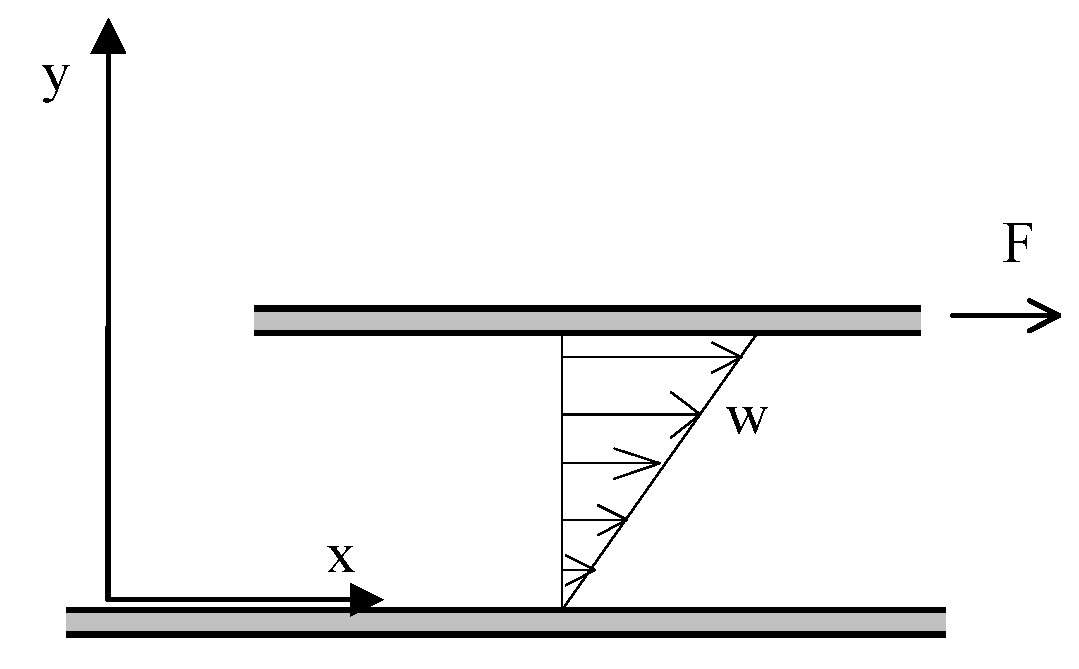
\includegraphics[width=0.6\textwidth]{fig/fluidodinamica/meato.eps}
    \caption{Azioni esercitate da un fluido tra due superfici in moto relativo \parencite{guglielmini2004lezioni}.} 
    \label{fig:meato}
\end{figure}
Il moto relativo tra fluido e parete è nullo, nel meato si crea quindi un campo di velocità triangolare, dove i piani di fluido scorrono l'uno sull'altro. Questo genera una forza resistente sulla superficie della parete superiore in moto. Indicando con \(A\) l'area della superficie di contatto tra  la lastra e il fluido, la forza resistente \(F\) è espressa in modulo dalla legge di Newton:
\[F= \mu \; A \; \frac{dw}{dy} \implies \tau_{yx} = \frac{F}{A} = \mu \; \frac{dw}{dy} \addtag \label{eq:newton} \]
in cui \(\mu\) è una proprietà del fluido detta viscosità dinamica e \(\tau_{yx}\) rappresenta lo sforzo di taglio viscoso ovvero la forza che agisce per unità di area su  una superficie interna al fluido in direzione parallela a tale superficie, e \(\frac{dw}{dy}\) è la derivata della velocità del fluido rispetto alla componente verticale del moto. Lo sforzo di taglio è proporzionale alla viscosità e al gradiente di velocità. Il rapporto è direttamente proporzionale se i fluidi sono classificabili come newtoniani, cioè se la viscosità è indipendente dallo sforzo viscoso per determinate condizioni di temperatura e pressione. Per i fluidi non newtoniani vale la seguente formula:
\[\frac{dw}{dy}=\frac{\tau}{\mu(\tau)}\addtag\label{eq:newtoniani}\]
A seconda dell'andamento della funzione \(\mu(\tau)\) i fluidi possono essere classificati come "pseudo plastici" o "dilatanti" (\figref{fig:newtoniani}).
\begin{figure}[htbp] %Immagine reologia di un fluido
    \centering
    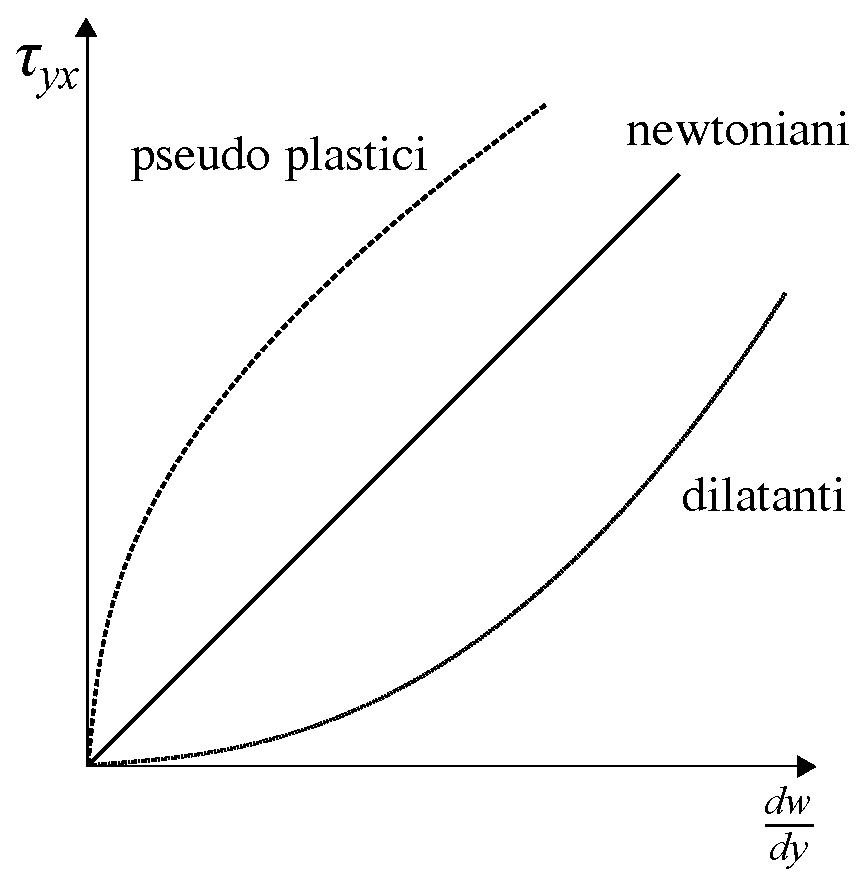
\includegraphics[width=0.6\textwidth]{fig/fluidodinamica/newtoniani.eps}
    \caption{Reologia di un fluido nel caso di fluidi newtoniani e non newtoniani \parencite{guglielmini2004lezioni}.} 
    \label{fig:newtoniani}
\end{figure}
\section[Moto e equazioni fondamentali]{Schematizzazione del moto e equazioni fondamentali di conservazione}
\sectionmark{Moto e equazioni fondamentali}
La rappresentazione analitica del moto di un fluido è assai complessa e richiede l'impiego di modelli al fine di semplificare la descrizione qualitativa e quantitativa di tale moto. Vengono indicate le tre figure fondamentali per la descrizione del moto di un fluido:
\begin{itemize}
\item \textbf{traiettoria di una particella}: il luogo dei punti occupati in tempi successivi dalla stessa particella fluida;
\item \textbf{linea di corrente} (o \textbf{linea di flusso}): è una linea che ha per tangente il vettore velocità in ogni punto;
\item \textbf{linea di fumo}: è il luogo dei punti occupati, ad un dato istante, dalle particelle che sono passate per uno stesso punto.
\end{itemize}
Nel caso di moto permanente questi  tre luoghi geometrici coincidono. Si definisce vena fluida o filetto di corrente l'insieme delle traiettorie le cui sezioni trasversali hanno velocità (perpendicolare alla sezione stessa), pressione, temperatura e volume specifico costanti.\\
Il modello di riferimento è quello di moto uni- o monodimensionale e si assumono condizioni di regime permanente di massa e termodinamico. In termini fisici il modello deve rispettare i principi di:
\begin{itemize}
\item \textbf{conservazione della massa};
\item \textbf{conservazione della quantità di moto};
\item \textbf{bilancio di energia}.
\end{itemize}

\paragraph{Conservazione della massa}
Si consideri un filetto di corrente in regime permanente. La massa di fluido $m$ che percorre, nell'unità di tempo, una qualunque generica sezione trasversale di area $A$ è costante. Quindi:
\[\dot{m}=wA\rho = costante\addtag\]
dove $\dot{m}$ è la portata di massa o portata massica, $w$ è la velocità e $\rho$ è la densità del fluido. Tra due distinte sezioni 1 e 2 la massa di fluido rimane costante:
\[w_1 A_1 \rho_1 = w_2 A_2 \rho_2\addtag\]
L'\textit{equazione di continuità}, o \textit{bilancio di massa}, può scriversi in forma differenziale come:
\[\frac{dw}{w} + \frac{dA}{A} + \frac{d\rho}{\rho} = 0\addtag\]

\paragraph{Bilancio della quantità di moto}
Si consideri un filetto di corrente in regime permanente a portata massica costante. Si consideri un volume di controllo C.V. (dall'inglese \textit{Control Volume}) compreso tra le sezioni 1 e 2, di massa $m$ più la massa $dm$ che attraversa la sezione 1 nel tempo $d\tau$. Di conseguenza nello stesso intervallo di tempo $d\tau$ una pari massa $dm$ attraversa la sezione 2. La variazione di quantità di moto è pari al prodotto della massa $dm$ per la differenza delle velocità tra le sezioni 1 e 2. Tale variazione di quantità di moto eguaglia l'impulso delle forze agenti sul C.V. (\figref{fig:quantitamoto}):
\[\sum{F\;d\tau}=dm(w_2-w_1)\qquad \textrm{ovvero}\qquad \sum{F}=\dot{m}(w_2-w_1)\]
dove \(\sum{F}\) è la risultante delle forze agenti sul C.V. nella direzione del moto.
\begin{figure}[htbp] %Immagine layout di mandata
    \centering
    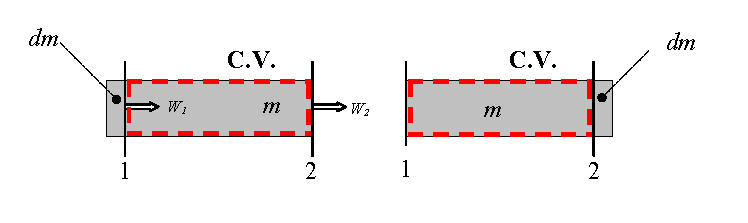
\includegraphics[width=\textwidth]{fig/fluidodinamica/quantitamoto.eps}
    \caption{Conservazione della quantità di moto a regime permanente.} 
    \label{fig:quantitamoto}
\end{figure}

\paragraph{Bilancio di energia e equazione di Bernoulli}
Tra le sezioni estreme di una generica vena fluida si applica l'equazione di bilancio dei sistemi aperti a regime permanente. Si considera come C.V. il volume racchiuso tra le due sezioni sopra citate. L'equazione di bilancio per unità di massa di un sistema aperto si può scrivere in forma differenziale come:
\[dQ-dL_e=dH+\frac{dw^2}{2}+gdz\addtag\]
dove $dQ$ e $dL_e$ rappresentano gli scambi di calore e di lavoro esterno netto attraverso la superficie di confine, $dH$ rappresenta l'entalpia, $z$ la quota potenziale e \(g\) la costante di gravitazione universale (\(g \simeq 9,81\) m/s\ap{2}). Poiché $dh=TdS_s+vdp$:
\[dL_e+TdS_s+v \; dp+\frac{dw^2}{2}+g \; dz\label{eq:intermediobernoulli}\addtag\]
dove $dS_s$ è la produzione entropica elementare e $v$ il volume specifico. Un qualunque lavoro specifico, può essere espresso come prodotto di un volume specifico per un'opportuna pressione differenziale $dp'$, per omogeneità dimensionale. Questa variazione di pressione differisce dalla variazione che il fluido subisce in moto. Sapendo che una qualsiasi pressione $p$ può essere espressa in termini di peso specifico $\gamma$ e altezza idrica $h$:
\[dL_e=v\;dp_e=v\;\gamma\;dh_e=g\;dh_e\addtag\label{eq:lavoroesterno}\]
Allo stesso modo per il lavoro di attrito:
\[dL_a=v\;dp_a=v\;\gamma\;dh_a=g\;dh_a\addtag\label{eq:lavoroattrito}\]
Se sostituiamo la \eqref{eq:lavoroesterno} e la \eqref{eq:lavoroattrito} nella \eqref{eq:intermediobernoulli} otteniamo:
\[dh_e+dh_a+\frac{dp}{\gamma}+\frac{dw^2}{2g}+dz=0\label{eq:bernoulligeneralizzata}\addtag\]
La \eqref{eq:bernoulligeneralizzata} è detta \textit{equazione di Bernoulli generalizzata} in forma differenziale e ha valenza energetica specifica (per unità di peso). I termini nella formula sono così nominati:
\begin{itemize}
    \item \(dh_e\) \textit{carico motore}, termine effettivo di scambio con l'esterno;
    \item \(dh_a\) \textit{carico d'attrito}, termine di dissipazione;
    \item \(\dfrac{dp}{\gamma}\) \textit{carico piezometrico}, l'effettiva variazione di pressione del fluido dovuta al moto;
    \item \(\dfrac{dw^2}{2g}\) \textit{carico cinetico};
    \item \(dz\) \textit{carico gravitazionale}, variazione di quota geodetica. 
\end{itemize}
Se la \eqref{eq:bernoulligeneralizzata} viene integrata tra la sezione 1 e la sezione 2 si ottiene:
\[(h_e)_{1,2}+(h_a)_{1,2}+\int^2_1{\frac{dp}{\gamma}}+\frac{w^2_2-w^2_1}{2g}+z_2-z_1=0\label{eq:bernoulliintegrata}\addtag\]
L'equazione caratterizzante il moto è così ridotta in termini di carichi differenziali, cioè in termini dimensionali si hanno delle lunghezze.\\
In caso di un condotto a pareti rigide, di sezione costante, orizzontale e attraversato da un fluido a regime permanente, cioè a carico motore e potenziale nullo, la \eqref{eq:bernoulliintegrata} diventa:
\[(h_a)_{1,2}+\int^2_1{\frac{dp}{\gamma}}+\frac{w^2_2-w^2_1}{2g}=0\label{eq:attritointermedio}\addtag\]
Se si ammettono trascurabili le variazioni di peso specifico rispetto alle variazioni di pressione, cioè si assume che il peso specifico sia costante, e la variazione di velocità nulla:
\[(h_a)_{1,2}=\frac{p_1-p_2}{\gamma}\label{eq:caricoattrito}\addtag\]
La \eqref{eq:caricoattrito} esprime il \textit{carico d'attrito} o in termini operativi la \textit{perdita di carico}. 
%%%%%%%%%%%%%%%%%%%%%%%%%%%%%%%%%%%%%%%%%%%%%%%%%%%%%%%%%%%%%%
\section{Calcolo delle cadute di pressione per attrito}
\subsection{Numero di Reynolds}
Si consideri un condotto rettilineo a pareti perfettamente lisce in cui scorre un fluido a velocità \(w\), di densità \(\rho\) e viscosità \(\mu\).\\
Si definisce \textit{moto laminare} (o \textit{viscoso} o \textit{regolare}) il moto dei fluidi caratterizzato dall'assenza di componenti caotiche. Le traiettorie effettive delle particelle risultano quindi regolari. Quando la corrente ha direzione rettilinea anche le traiettorie sono rettilinee e ad esse si raccordano quando, per esempio, la presenza di una condotta curva impone deviazioni della direzione.\\
Incrementando la velocità media di portata si denota che le traiettorie delle particelle fluide tendono a non mantenere direzione parallela all'asse della condotta. Tale moto è definito \textit{turbolento} e può essere inteso come la somma di due tipi di movimento: al \textit{moto di trasporto}, diretto secondo l'asse della tubazione, si sovrappone un movimento caotico e disordinato definito \textit{moto di agitazione}.\\
Reynolds fu il primo a definire che il tipo di moto dovesse dipendere non solo dalla velocità ma anche dalla densità e viscosità del fluido oltre che alla geometria della condotta. Il \textit{numero di Reynolds} è così definito:
\[Re=\frac{\rho \; w \; D}{\mu}\addtag\label{eq:reynolds}\]
Il numero di Reynolds definisce il tipo di moto che si instaura in condotta:
\begin{itemize}
    \item per \(Re<2000\qquad\)il moto in un condotto è laminare;
    \item per \(2000<Re<10000\qquad\)si ha una regione di transizione;
    \item per \(Re>10000\qquad\)il moto in un condotto è completamente turbolento.
\end{itemize}
%%%%%%%%%%%%%%%%%%%%%%%%%%%%%%%%%%%%%%%%%%%%%%%%%%%%%%%%%%%%%%
\subsection{Fattore di attrito di Moody}
Sia in condizioni di moto laminare che in condizioni di moto turbolento la caduta di pressione totale dipende dalle caratteristiche del fluido,  del moto e della condotta. In breve, il carico di attrito dipende da parametri:
\begin{itemize}
    \item \textbf{fisici} - \(\mu\) e \(\rho\) - relativi ai fluidi in movimento;
    \item \textbf{cinematici} - \(w\) - caratterizzanti il trasporto di massa fluida;
    \item \textbf{geometrici} - \(D\) e \(\epsilon\) - legati alla tubazione e alla \textit{scabrezza assoluta} della parete interna della condotta.
\end{itemize}
Perciò si può affermare che:
\[\frac{\Delta p}{l}=f(\rho, \; \mu, \; w, \; D, \; \epsilon) \addtag \label{eq:funzcaduta} \]
dove \(l\) è la lunghezza della condotta. L'equazione di Darcy-Weisbach può essere definita sia in funzione delle perdite di carico piezometriche \eqref{eq:darcyweisbachH} sia in funzione delle cadute di pressione \eqref{eq:darcyweisbachP}:
\[h_a = \lambda \; \frac{l}{D} \; \frac{w^2}{2 \; g} \addtag \label{eq:darcyweisbachH} \]
\[\Delta p_a = \lambda \; \frac{l}{D} \; \frac{\rho \; w^2}{2} \addtag \label{eq:darcyweisbachP} \]
dove \(\lambda\) è detto \textit{fattore d'attrito di Moody} o \textit{indice di resistenza}. La perdita di carico corrispondente, per un certo valore \(\lambda\), risulta proporzionale al carico cinetico e alla lunghezza del condotto. In regime di moto laminare il fattore di attrito è proporzionale al solo coefficiente di Reynolds:
\[\lambda=\frac{64}{Re} \addtag \]
In regime tubolento l'indice di resistenza è legata alla rugosità della parete. Il rapporto \(\frac{\epsilon}{D}\) è definito \textit{scabrezza relativa}. La relazione funzionale equivalente è:
\[\lambda=f \; \left(Re, \; \frac{\epsilon}{D}\right) \addtag \]
Sulla base dei risultati sperimentali al variare dei parametri del modello di flusso in condotta in regime turbolento, è stato costituito il \textit{diagramma di Moody} (\figref{fig:moody}). Gli andamenti all'interno di tale diagramma sono la rappresentazione grafica della \textit{correlazione di Colebrook}:
\[ \frac{1}{\sqrt{\lambda}} = - 2 \ln \left( \frac { \epsilon/D} {3{,}71} + \frac {2{,}51} {Re \, \sqrt{\lambda}} \right) \addtag \label{eq:colebrook} \]

\begin{figure}[htbp] %Immagine diagramma di Moody
    \centering
    \includegraphics[width=.9\textwidth]{fig/fluidodinamica/moody.eps}
    \caption{Diagramma di Moody per il calcolo del fattore di attrito in condotta.} 
    \label{fig:moody}
\end{figure}

Il fattore di attrito può essere espresso anche tramite il \textit{numero di Fanning} \(f\), adimensionale e definito come il rapporto tra gli sforzi di taglio e le forze di inerzia:
\[f=\dfrac{2\tau}{\rho w^2} \addtag \label{fanning} \]
Il fattore di attrito di Moody è quattro volte il numero di Fanning:
\[\lambda = 4f \addtag \label{eq:fanningmoody} \]
Blasius propone il calcolo del numero di Fanning a partire dal numero di Reynolds:
\[f=\dfrac{0,079}{Re^{0,25}} \addtag \label{eq:fanningreynolds} \]
La \eqref{eq:fanningreynolds} è applicabile in condizione di tubi a pareti interne lisce (scabrezza nulla, \(\epsilon=0\)) e regime di flusso non totalmente turbolento (\(Re<10^5\)).
%%%%%%%%%%%%%%%%%%%%%%%%%%%%%%%%%%%%%%%%%%%%%%%%%%%%%%%%%%%%%%%%%%%%%%
\subsection{Perdite di carico per un liquido}
Una relazione approssimativa per la valutazione delle perdite di carico di liquidi in condotta è quella di Hazen-Williams.  Questa relazione è valida solo per acqua in condizioni di regime turbolento a temperatura compresa tra i 4°C e 25°C.
\[\frac{h_a}{l} = \frac{10,65\ Q^{1,85}}{C^{1,85}\ d^{4,87}} \addtag \label{eq:HW}\]
dove \(Q\) è la \textit{portata volumetrica}, la costante moltiplicativa numerica 10,65 non è adimensionale (ha le dimensioni di \(s^{1,85}/m^{0,86}\)) e la costante adimensionale \(C\) è un valore tabellato.
\begin{table}[htbp]
    \small
    \centering
    \begin{tabular}{|l|r|}
        \hline
        \textbf{Tipologia tubo} & \(\mathbf{C}\)\\
        \hline
             Tubi estremamente lisci & 140\\
        Tubi nuovi, acciaio o ghisa & 130\\
        Tubi in legno o calcestruzzo & 120\\
        Tubi in acciaio rivettato, nuovi & 110\\
        Tubi vecchi in ghisa, mattoni & 100\\
        Tubi in acciaio rivettato, vecchi & 95\\
        Tubi in acciaio corroso & 80\\
        Tubi in acciaio fortemente corroso & 60\\
        \hline
    \end{tabular}
    \label{tab:coefficientiHZ}
    \caption{Coefficienti $C$ adimensionali per la formula di Hazen-Williams.}
\end{table}
L'equazione fornisce direttamente il valore delle perdite di carico distribuite per unità di lunghezza della tubazione in funzione della portata volumetrica e del diametro idraulico. Se ora esplicitiamo la \eqref{eq:darcyweisbachH} in funzione del diametro interno \(D\), ponendo la \textit{portata volumetrica} come \(Q=w \, A\):
\[h_a = \lambda \; \frac{l}{D} \; \frac{w^2}{2 \; g} \quad \implies \quad \frac{h_a}{l}=\frac{8 \, f}{\pi^2 \, 2g} \, \frac{Q^2}{D^5} \addtag \label{eq:darcyweisbachespl} \]
In entrambe le formulazioni (la forma generale delle perdite di carico e l'apporssimazione di Hazen-Williams) si rileva che, a parità di portata, le perdite di carico sono inversamente proporzionali al diametro della tubazione elevato ad un esponente prossimo a 5.

%%%%%%%%%%%%%%%%%%%%%%%%%%%%%%%%%%%%%%%%%%%%%%%%%%%%%%%%
\subsection{Perdite di carico per un gas}
In condotte lunghe, il flusso di un gas è prossimo alle condizioni isotermiche. Le cadute di pressione in tali linee sono spesso grandi paragonate alla pressione in ingresso e il problema non può essere trattato tramite il modello di flusso di Darcy. Una soluzione accurata è data dall'equazione:
\[\dot{m}^2=\left[\dfrac{A^2}{v_1\left(\dfrac{\lambda\,l}{D}+2\ln\dfrac{p_1}{p_2}\right)}\right]\left[\dfrac{{p_1}^2-{p_2}^2}{p_1}\right] \addtag \label{eq:cpgasgenerale1}\]
dove \(p_1\) e \(p_2\) sono le pressioni all'inizio e alla fine della condotta.
Se esplicitiamo nella \eqref{eq:cpgasgenerale1} il volume specifico in ingresso \(v_1\) utilizzando l'equazione di stato di un gas reale:
\[{p_1}^2-{p_2}^2=Z_m R T \left(\dfrac{w}{A}\right)^2\left(\lambda \, \dfrac{l}{D}+2\ln\dfrac{p_1}{p_2}\right)  \addtag \label{eq:cpgasgenerale2}\]
dove \(Z_m\) è il \textit{fattore di comprimibilità del gas}, \(R\) è la \textit{costante universale dei gas perfetti} e \(T\) la temperatura.
Si formulino le seguenti assunzioni:
\begin{itemize}
    \item flusso di gas a condizioni isotermiche;
    \item assenza di lavoro meccanico in ingresso e uscita;
    \item regime permanente;
    \item gas perfetto;
    \item velocità come rappresentazione della velocità media nella sezione trasversale;
    \item coefficiente d'attrito \(\lambda\) costante;
    \item condotta dritta e orizzontale
\end{itemize}
La \eqref{eq:cpgasgenerale1} e la \eqref{eq:cpgasgenerale2} possono essere scritte semplificate in:
\[\dot{m}^2=\left[ \dfrac{D \, A^2}{v_1 \, \lambda \, l}\right] \left[\dfrac{{p_1}^2-{p_2}^2}{p_1}\right] \addtag \label{eq:cpgassempl1} \]

\[{p_1}^2-{p_2}^2=Z_m R T \left(\dfrac{w}{A}\right)^2\left(\lambda \, \dfrac{l}{D}\right)  \addtag \label{eq:cpgassempl2}\]
Possono essere utilizzate tre diverse forme semplificate per il calcolo delle portate di gas in condotta, a seconda delle specifiche tecniche dell'infrastruttura.

\paragraph{Equazione di Weymouth}
L'equazione di Weymouth è raccomandata per condotte con diametro piccolo (generalmente sotto i 12") e lunghezza limitata (sotto i 30 km) all'interno delle batterie di produzione o per le linee di raccolta secondarie, pressione medio-alta (compresa tra 7 bar e 70 bar) in regime di moto turbolento (alto valore del numero di Reynolds).
\[Q_h=2,61\e{-8} \; {d_{mm}}^{2,667} \; \left[ \left(\dfrac{p_1^2 - p_2^2}{\rho_r \, l_{km}}\right) \dfrac{288}{T_1} \right]^{0.5} \addtag \label{eq:weymouth} \]
dove \(Q_h\) è la portata espressa in Smc\footnote{\textit{Standard metri cubi}, quantità di gas contenuta in un 1 m\ap{3} a condizioni standard di pressione (\(p=101325\) Pa, pressione ambientale) e di temperatura  (\(T=288,15\) K, 15°C)}/h, \(\rho_r\) è la densità relativa, \(d_{mm}\) è il diametro interno della condotta espresso in mm, \(l_{km}\) è la lunghezza della condotta espressa in km.

\paragraph{Equazione di Panhandle}
L'equazione di Panhandle è indicata per condotte di grande diametro (pari o sopra i 12"), condotte lunghe (più di 70 km) e per valori del numero di Reynolds moderati. 
\[Q_h=2,044\e{-8} \; E \;{d_{mm}}^{2,6182} \; \left( \dfrac{p_1^2 - p_2^2}{l_{km}} \right)^{0,5394} \addtag \label{eq:pandhandle} \]
dove \(E\) rappresenta il fattore di efficienza del flusso (\(E \leq 1\), ha valore unitario in caso di nuove condotte)

\paragraph{Equazione di Spitzglass}
Esistono due versioni di questa equazione: ad alta o bassa pressione. L'equazione di Spitzglass relativa a condotte a bassa pressione è:
\[Q_h = 9,50 \; \left[ \dfrac{(p_1-p_2) \; {d_{mm}}^5 }{l_{mm} \; \rho_r \; (1+0,09144/d_{mm} + 1,1811 \; d_{mm}) } \right]^2 \addtag \label{eq:spitzglass}\]


\subsection{Perdite di carico concentrate}
Il fluido, lungo il suo percorso in condotta, può incontrare brusche variazioni di sezione, direzione o ostruzioni come filtri o rubinetti. Il calcolo delle resistenze puntuali è difficilmente calcolabile in modo analitico e ci si basa maggiormente su dati puramente sperimentali. Tutte le resistenze relative a diversi elementi tipici della condotta sono espresse in funzione del carico cinetico:
\[\Delta p' = \gamma \; \frac{w^2}{2g} \; f' \addtag \label{eq:concentrate}\]
dove \(f'\) assume valori diversi a seconda del tipo di singolarità. La somma di perdite di carico concentrate e distribuite fornisce la caduta di pressione totale per una generica condotta percorsa da un fluido.

%%%%%%%%%%%%%%%%%%%%%%%%%%%%%%%%%%%%%%%%%%%%%%%%%%%%%%%%%%
\section{Moto multifase}
In termodinamica classica si definisce \textit{fase} come uno stato macroscopico della materia omogeneo per struttura fisica e composizione chimica. I \textit{flussi bifase} sono caratterizzati dalla presenza di due fasi e rappresentano il caso più semplice di \textit{flusso multifase} o multicomponente. Nei flussi bifase, l'iterazione tra le due fasi porta alla formazione di particolari regimi di flusso. Il verificarsi di un determinato regime dipende dalla portata, dalle caratteristiche fisiche e dalle condizioni termodinamiche delle due fasi e dalle caratteristiche fisiche dell'impianto.

\subsection{Regime di flusso in condotta}
L'inclinazione della condotta incide fortemente sulla formazione dei diversi regimi di flusso: in caso di tubazioni verticali, la forza gravitazionale agisce nella stessa direzione della forza inerziale, quindi lungo l'asse della condotta. In condotte verticali si hanno quindi regimi pseudo-simmetrici rispetto l'asse della condotta, in tubazioni orizzontali la fase liquida e la fase gassosa tendono a disporsi rispettivamente sulla parte inferiore e superiore. 

\subsubsection{Condotte verticali} \label{sssec:verticali}
I regimi di flusso bifase per condotte verticali sono così classificati (\figref{fig:verticale}):
\begin{itemize}
    \item flusso a bolle;
    \item flusso a slug;
    \item flusso a churn o agitato;
    \item flusso anulare misto.
\end{itemize}

\begin{figure}[htbp]
\centering
    \subfloat[][Flusso a bolle]
    {\makebox[0.2\textwidth]{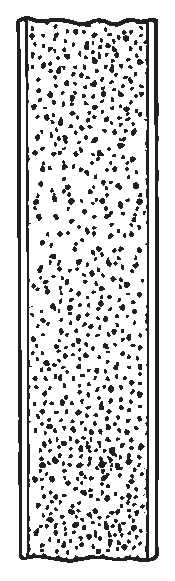
\includegraphics[width=.1\textwidth]{fig/fluidodinamica/vertical/ver-bubble.eps}} \label{fig:ver-bubble}} \quad
    \subfloat[][Flusso a slug]
    {\makebox[0.2\textwidth]{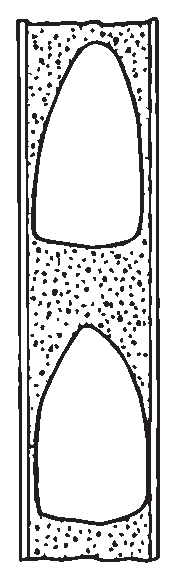
\includegraphics[width=.1\textwidth]{fig/fluidodinamica/vertical/ver-slug.eps}} \label{fig:ver-slug}}  \quad
    \subfloat[][Flusso a churn o agitato]
    {\makebox[0.2\textwidth]{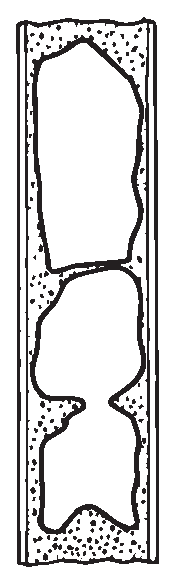
\includegraphics[width=.1\textwidth]{fig/fluidodinamica/vertical/ver-annular.eps}} \label{fig:ver-churn}} \quad
    \subfloat[][Flusso anulare misto]
    {\makebox[0.2\textwidth]{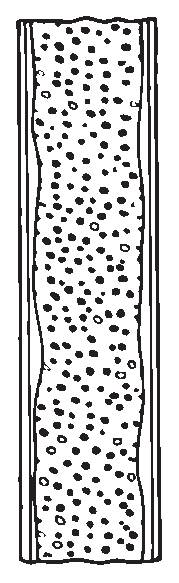
\includegraphics[width=.1\textwidth]{fig/fluidodinamica/vertical/ver-mist.eps}} \label{fig:ver-annular} }
\caption{Regimi di flusso bifase in condotte verticali}
\label{fig:verticale}
\end{figure}

Per comprendere nel dettaglio i vari regimi che si possono instaurare in condotta si fa riferimento alla mappa dei regimi di flusso bifase avvallata da \citeauthor{griffith1984multiphase} per condotte verticali (\figref{fig:ver-griffith}).

\begin{figure}[htbp]
    \centering
    \includegraphics[width=.6\textwidth]{fig/fluidodinamica/ver-griffith.eps}
    \caption{Mappa per regimi di flusso bifase per condotte verticali \parencite{griffith1984multiphase}.}
    \label{fig:ver-griffith}
\end{figure}

Per basse velocità superficiali della fase gassosa, avviene in condotta il solo regime a bolle (\figref{fig:ver-bubble}). In questo regime la fase liquida si muove a velocità uniforme mentre le bolle di gas sono più veloci o più lente a seconda del loro diametro. Se si incrementa la velocità della fase gassosa, questa tenderà a viaggiare di pari passo alla fase liquida, creando così il regime a slug (\figref{fig:ver-slug}) e il regime a churn o anche detto agitato (\figref{fig:ver-churn}), dove ormai l'effetto della fase gassosa è predominante rispetto alla fase liquida. Nel regime anulare misto (\figref{fig:ver-annular}) la fase gassosa è continua e la fase liquida è dispersa nel gas oppure disposta sulle pareti interne.

\subsubsection{Condotte orizzontali}
I regimi di flusso in condizioni di condotta orizzontale possono essere così classificati (\figref{fig:orizzontale}):
\begin{itemize} 
    \item flusso stratificato;
    \item flusso a onde;
    \item flusso a plug o a bolle allungate;
    \item flusso a slug;
    \item flusso anulare;
    \item flusso a bolle disperse.
\end{itemize} 

\begin{figure}[htbp]
\centering
    \subfloat[][Flusso stratificato]
    {\includegraphics[width=.4\textwidth]{fig/fluidodinamica/horizontal/hor-stratified.eps} \label{fig:hor-stratified}} \qquad \qquad
    \subfloat[][Flusso a onde]
    {\includegraphics[width=.4\textwidth]{fig/fluidodinamica/horizontal/hor-wavy.eps} \label{fig:hor-wavy}} \\
    \subfloat[][Flusso a plug]
    {\includegraphics[width=.4\textwidth]{fig/fluidodinamica/horizontal/hor-plug.eps} \label{fig:hor-plug}} \qquad \qquad
    \subfloat[][Flusso a slug]
    {\includegraphics[width=.4\textwidth]{fig/fluidodinamica/horizontal/hor-slug.eps} \label{fig:hor-slug}}\\
    \subfloat[][Flusso anulare]
    {\includegraphics[width=.4\textwidth]{fig/fluidodinamica/horizontal/hor-annular.eps} \label{fig:hor-annular}} \qquad \qquad
    \subfloat[][Flusso a bolle disperse]
    {\includegraphics[width=.4\textwidth]{fig/fluidodinamica/horizontal/hor-bubble.eps} \label{fig:hor-bubble}}
\caption{Regimi di flusso bifase in condotte orizzontali}
\label{fig:orizzontale}
\end{figure}
Per la determinazione dei diversi regimi di flusso bifase aria-acqua si fa riferimento alle mappe per condotte orizzontali proposte da \textcite{griffith1984multiphase}, \textcite{baker1954simultaneous} e \textcite{taitel1976model}.

\paragraph{\textcite{griffith1984multiphase}}
Il regime di flusso è definito tramite la \textit{velocità superficiale} \(w_i\), legata alla portata volumetrica della fase i-esima attraverso una generica sezione \(A\) della condotta. Si ha quindi:
\[w_G = \frac{Q_G}{A} \addtag\]
\[w_L = \frac{Q_L}{A} \addtag\]
dove i pedici \(g\) e \(l\) fanno riferimento alla fase gassosa o liquida. Le linee continue interne rappresentano la transizione tra i diversi regimi.\\
Per basse velocità superficiali della fase liquida si verificano flussi stratificati a interfaccia liscia (\figref{fig:hor-stratified}), a onda (\figref{fig:hor-wavy})e anulare misto (\figref{fig:hor-annular}) a seconda della velocità superficiale del liquido. Questi tre regimi fanno parte della categoria dei flussi separati: le due fasi appaiono come due flussi continui senza apparente iterazione. Il flusso stratificato e quello a onde sono caratterizzati dallo scorrimento della fase liquida nella parte inferiore della condotta, in quello anulare la fase liquida si dispone lungo le pareti interne della condotta. All'aumentare della velocità superficiale della fase liquidi, si osserva un maggiore miscelamento delle due fasi e si verificano  flussi a slug o a bolle allungate (\figref{fig:hor-slug}) o flussi a plug (\figref{fig:hor-plug}). La differenza tra questi due regimi è sottile: nel flusso a slug sono disperse numerose bollicine di gas nella fase liquida, al contrario del flusso a plug. Ad alte velocità superficiali della fase liquida si verifica il flusso a bolle (\figref{fig:hor-bubble}), caratterizzato dalla presenza di bolle di gas disperse nella fase liquida.
\begin{figure}[htbp]
    \centering
    \includegraphics[width=.6\textwidth]{fig/fluidodinamica/hor-griffith.eps}
    \caption{Mappa di \textcite{griffith1984multiphase}) per regimi di flusso bifase per condotte orizzontali.}
    \label{fig:hor-griffith}
\end{figure}

\paragraph{\textcite{baker1954simultaneous}}
La mappa di \textcite{baker1954simultaneous} per condotte orizzontali con flusso bifase \figref{fig:baker} è stata proposta originariamente sia per Sistema Internazionale che per sistema consuetudinario statunitense. Per l'utilizzo della mappa devono essere determinati i parametri adimensionali \(\Lambda\) e \(\Psi\) e la \textit{velocità di massa} o \textit{flusso di massa} \(j_i\), la massa della fase i-esima che attraversa una generica sezione trasversale \(A\) della condotta:
\[j_G = \frac{\dot{m_G}}{A}=\frac{\rho_G w_G A}{A}=\rho_G w_G \addtag\]
\[j_L = \frac{\dot{m_L}}{A}=\frac{\rho_L w_L A}{A}=\rho_L w_L \addtag\]
dove \(j_G\) e \(j_L\) sono (in modulo) la velocità di massa del gas e del liquido. I parametri adimensionali \(\Lambda\) e \(\Psi\) sono definiti da:
\[\Lambda= \left(\dfrac{\rho_G}{\rho_{aria}} \dfrac{\rho_L}{\rho_{acqua}}\right)^{1/2} \addtag \label{eq:lambdabaker} \]
\[\Psi=\left( \frac{\sigma_{acqua}}{\sigma} \right) \left[ \left( \frac{\mu_L}{\mu_{acqua}} \right) \left( \frac{\rho_{acqua}}{\rho_L} \right)^2 \right]^{1/3} \addtag \]
dove \(\rho_G\), \(\rho_L\), \(\mu_L\) e \(\sigma\) sono proprietà proprie del fluido. I termini noti, quindi le proprietà di riferimento sono:
\begin{itemize}
    \item \(\rho_{acqua}=1000\) kg/m\ap{3};
    \item \(\rho_{aria}=1,23\) kg/m\ap{3};
    \item \(\mu_{acqua}=0,001\) N sec/m\ap{2};
    \item \(\sigma_{acqua}=0,072\) N/m.
\end{itemize}
I valori sugli assi x e y sono così identificati. L'intersezione sulla mappa fornisce il regime bifase che si instaura nella condotta sulla base del modello.
\begin{figure}[htbp]
    \centering
    \includegraphics[width=.6\textwidth]{fig/fluidodinamica/baker.eps}
    \caption{Mappa di \textcite{baker1954simultaneous}) per regimi di flusso bifase per condotte orizzontali.}
    \label{fig:baker}
\end{figure}

\paragraph{\textcite{taitel1976model}}
Nel lavoto di \textcite{taitel1976model} (\figref{fig:taitel}) si propone una mappa per condotte orizzontali che nasce dalla combinazione di analisi analitiche e selezione empirica di numerosi parametri di riferimento. La mappa usa il \textit{parametro di Martinelli} \(\chi\), il \textit{numero di Froude} del gas \(Fr_G\) e i parametri \(T\) e \(K\).

\begin{figure}[htbp]
    \centering
    \includegraphics[width=.6\textwidth]{fig/fluidodinamica/taitel.eps}
    \caption{Mappa di \textcite{taitel1976model}) per regimi di flusso bifase per condotte orizzontali. Gli assi di riferimento cambiano a seconda della curva considerata, come descritto nel pannello al di sotto del grafico.}
    \label{fig:taitel}
\end{figure}

Il parametro di Martinelli è dato dalla radice quadrata del rapporto tra i gradienti di pressione del liquido e del gas:
\[\chi = \left[ \frac{(dp/dl)_L}{(dp/dl)_G} \right]^{1/2} \addtag \label{eq:martinelli} \]
Si ricorda che il gradiente di pressione per unità di lunghezza è dato dalla derivata dell'equazione di Darcy-Weisbach \eqref{eq:darcyweisbachP} in funzione della caduta di pressione lungo la direzione della condotta:
\[\Delta p_{a,k} = \lambda_k \; \frac{l}{D} \; \frac{\rho_k \; w_k^2}{2} \implies \left(\dfrac{dp}{dl}\right)_k =- \frac{\lambda_k}{D} \; \frac{\rho \; w^2}{2} = - \frac{\lambda_k \; j_k^2}{\rho_k \; D}  \addtag \label{eq:gradientepressione} \]
Il numero di Froude è un gruppo adimensionale e rappresenta la frazione liquida di un fluido.  Dal punto di vista analitico mette in relazione forza di inerzia con la forza peso. Per la fase gassosa vale:
\[Fr_G = \frac{j_G}{[\rho_G(\rho_L-\rho_G)D \; g]^{1/2}} \addtag \label{eq:froude}\]
Il parametro \(T\) è definito come:
\[ T = \left[ \dfrac{|(dp/dl)_L|}{g(\rho_L-\rho_G)} \right]^{1/2} \addtag \label{parametroT} \]
Il parametro \(K\) invece è funzione del numero di Froude del gas e del numero di Reynolds del liquido:
\[K=Fr_G \; Re_L^{1/2} \addtag \label{parametroK} \]
Caratteristica principale di questa mappa di regime è l'impiego di diverse coordinate, in funzione dei parametri trovati, a seconda della curva a cui si fa riferimento. Dapprima si calcolano quindi il parametro di Martinelli \(\chi\) e il numero di Froude del gas \(Fr_G\). Se le coordinate del punto trovato ricadono nella parte superiore della curva A, rappresentata rispetto al sistema di coordinate \(Fr_G-\chi\), il regime sarà quindi anulare. Nel caso in cui il punto si collochi al di sotto della curva viene calcolato il parametro \(K\). Facendo riferimento alla curva C e quindi al sistema di coordinate \(K-\chi\) il regime sarà a onde o stratificato con interfaccia liscia se il punto trovato è rispettivamente nella parte superiore o inferiore della curva C. Se il punto ricade nella parte superiore a destra del grafico, si fa riferimento alla curva D, quindi al sistema di coordinate \(T - \chi \). Il regime sarà a bolle disperse se il punto trovato si trova al di sopra della curva D, viceversa il regime sarà di natura intermittente o a slug. \\ \\
Tutti i modelli fin qui presentati sono stati sviluppati per flussi bifase in condizioni adiabatiche. Tuttavia questi modelli, tramite accorgimenti di natura analitica, posso risponde anche a condizioni diabatiche, cioè ipotizzando la condotta come sistema aperto in cui avviene scambio di calore con l'esterno. Lo studio dei regimi di flusso può quindi essere esteso, per esempio, negli impianti di refrigerazione oppure negli scambiatori termici.

\subsection{Cadute di pressione per attrito di un flusso bifase}
Si può semplificare lo studio del moto di un fluido bifase se si assume che le fasi siano ben miscelate fra loro, quindi come un unico fluido monofase. Il \textit{modello omogeneo} può essere applicato quando le fasi sono fortemente interdisperse tra loro, cioè quando entrambe le fasi hanno velocità superficiali sostenute. Le perdite di carico totali \(\Delta p_{tot}\) sono la somma delle perdite di carico statiche o gravitazionali \(\Delta p_s\), le perdite di carico della quantità di moto \(\Delta p_{mom}\) e le perdite di carico per attrito \(\Delta p_a\): 
\[\Delta p_{tot} = \Delta p_s +\Delta p_{mom} + \Delta p_a \addtag \label{eq:perditetot}\]
La perdita di carico statico per un fluido bifase omogeneo è:
\[\Delta p_s = \rho_H \; g \; z\ \addtag \]
dove \(z\) è la differenza di quota geodetica tra le sezioni di ingresso e uscita della condotta, o meglio l'altezza della condotta. Per densità omogenea \(\rho_H\) si intende:
\[\rho_H=\rho_L(1-\epsilon_H)+\rho_G \; \epsilon_H \addtag \label{eq:omogenea} \]
Si determina la frazione di vuoto \(\epsilon_h\) in funzione del titolo di vapore \(x\):
\[\epsilon_H = \left[ 1+ \left( \dfrac{w_G}{w_L} \dfrac{(1-x)}{x} \dfrac{\rho_G}{\rho_L} \right) \right]^{-1} \addtag \]
dove il rapporto \(w_G/w_L\) è detto \textit{rapporto di slittamento} e ha valore unitario nel caso di flussi omogenei. Il gradiente di pressione della quantità di moto per unità di lunghezza del condotto è:
\[\left( \dfrac{dp}{dl} \right)_{mom}=\dfrac{d(j_{tot}/\rho_H)}{dz} \addtag \]
Il punto cruciale del calcolo delle cadute di pressione per un flusso bifase risiede nella stima del termine di attrito, in questo frangente rappresentato dal numero di Fanning \(f\). Se si esprime la \eqref{eq:darcyweisbachP} in funzione del numero di Fanning \(f_{tot}\) per un flusso bifase, in funzione del flusso di massa \(j_{tot}\):
\[\Delta p_a = \dfrac{2 \; f_{tot} \; j_{tot}^2}{\rho_{tot}} \; \dfrac{l}{D} \addtag \label{eq:darcyweisbachfanning2f} \]
Si può esprimere il numero di Fanning tramite la \eqref{eq:fanningreynolds}, il numero di Reynolds per mezzo della \eqref{eq:reynolds}. Come viscosità, parametro utile al calcolo del numero di Reynolds, può essere scelta quella della fase liquida oppure una media pesata in base al titolo di vapore \(x\):
\[\mu_{tot} =x \; \mu_G + (1+x) \; \mu_L \addtag \]
\\
\'E importante acquisire le basi della fluidodinamica multifase per capire come le iterazioni tra le diverse fasi e le perdite di carico definiscano il flusso che si instaura in condotta. L'ingegneria petrolifera ha cercato negli anni di affinare i modelli interpretativi, così da avvicinare le stime di produzione di un pozzo ai trend reali. In particolar modo, la corretta interpretazione del moto multifase per i pozzi a gas determina la tipologia e la configurazione di sistemi per l'aumento di portata o la diminuzione delle perdite di carico. Si intuisce quindi che l'aumento delle performance è legato alla veridicità del modello calcolato. Nel prossimo capitolo sono trattati i problemi di un pozzo a gas legati a condizioni di flusso multifase e le tecnologie oggi utilizzate per ovviare al calo di rendimento nel tempo.
%\section{Moto dei fluidi comprimibili in condotta a sezione variabile}
%\subsection{Velocità del suono}
%\subsection{Equazione di Hugoniot e numero di Mach}
%\subsection{Propagazione dei disturbi in flussi subsonici e supersonici}
%\subsection{Proprietà al ristagno}
%\subsection{Flusso attraverso un'onda d'urto normale}


\clearpage{\pagestyle{empty}\cleardoublepage}
\chapter{Applicazioni di schiumogeno per l'ottimizzazione della produzione degli idrocarburi}
\chaptermark{Applicazioni di schiumogeno}
\
\section{Introduzione}
Per \textit{Gas Well Deliquification} o \textit{Gas Well Dewatering} si intende l'insieme delle tecnologie e delle applciazioni utili alla rimozione di acqua o condensati in fase produttiva da un pozzo a gas. Nello specifico il concetto di GDW racchiude tutti gli strumenti utili nel combattere il fenomeno del \textit{liquid loading}, definito come l'impossibilità di un pozzo a gas di rimuovere liquidi prodotti in pozzo. 

\section{Liquid loading}
\subsection{Ciclo di vita di un pozzo a gas}
Nel paragrafo \ref{sssec:verticali} si è discusso dei diversi tipi regimi di flusso bifase per condotte verticali. Un pozzo a gas può presentare tutti i regimi di flusso: in \figref{fig:wellhistory} è possibile comprendere graficamente l'evoluzione del pozzo durante il suo ciclo di vita.

\begin{figure}[htbp]
    \centering
    \includegraphics[width=.8\textwidth]{fig/foamer/wellhistory.eps}
    \caption{Schematizzazione del ciclo di vita di un pozzo a gas}
    \label{fig:wellhistory}
\end{figure}

Generalmente in un pozzo sono presenti tutti i diversi regimi di flusso, con il passare del tempo varia la distribuzione dei diversi pattern lungo il tubino di produzione. Inizialmente il gas è fase dominante nel pozzo e ha forza sufficiente per trascinare tutto il liquido presente fondo pozzo. Ad alte velocità superficiali del gas corrisponde un regime anulare misto: la fase liquida è interdispersa nella fase gassosa. Con il diminuire della velocità del gas nel tempo, la fase liquida comincia a precipitare e a depositarsi sul fondo, ostacolando la normale produzione di gas.

\subsection{Problemi legati al liquid loading}
Il liquid loading porta a un regime di flusso a slug e a una produzione di gas discontinua e inferiore. Se il gas ha energia sufficiente a rimuovere i liquidi presenti a fondo pozzo, la portata del gas risponde in modo corretto alla stima di produzione rispetto al tempo di vita del pozzo, definita per via grafica dalla \textit{Decline Curve Analysis} (DAC).

CORREGGERE IMMAGINE, INTRODURRE IN ORDINATA PORTATA
\begin{figure}[htbp]
    \centering
    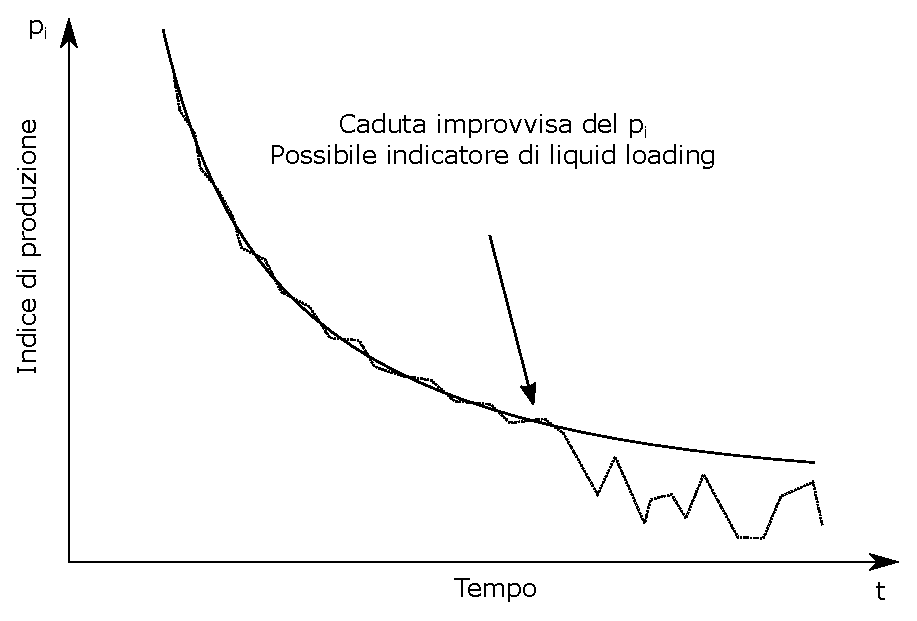
\includegraphics[width=.8\textwidth]{fig/foamer/declinecurve.eps}
    \caption{Analisi della curva di declino.}
    \label{fig:ipr}
\end{figure}

In caso di aumento della colonna idrostatica, il pozzo produce gas in quantità minore rispetto alle stime effettuate. Raggiunto uno stato critico di produzione di gas, il giacimento non ha più energia sufficiente per lo spiazzamento del pozzo e l'effetto combinato di precipitazione di liquidi a fondo pozzo e diminuzione fisiologica della pressione di giacimento porta all'innalzamento della colonna idrostatica. L'aumento dell'altezza della colonna di liquido può quindi terminare la produzione, sancendo così il termine del ciclo di vita del pozzo stesso.
 
\subsection{Sorgenti di liquidi per un pozzo a gas}
Nella maggior parte dei pozzi la produzione di gas è associata a produzione di liquidi. Questi liquidi possono essere acqua, vapore acqueo condensato o idrocarburi condensati. I liquidi prodotti in pozzo dipendono dalle condizioni e dal tipo di giacimento in questione. Le principali cause possono essere:

\begin{itemize}
    \item \textbf{\textit{water coning}}: in un giacimento caratterizato da una falda a gas collocata su una falda d'acqua, alti valori di produzione di gas corrispondono a una repentina caduta di pressione locale; la superficie di separazione delle due fasi assume la configurazione di un conoide e la fase liquida invade così la perforazione;
    \item \textbf{acqua da acquifero}: se la coltivazione del giacimento avviene per mezzo della spinta dell'acquifero (\textit{water-drive}) l'acqua può viaggiare fino a raggiungere la perforazione;
    \item \textbf{vapore acqueo condensato}: poiché nei giacimenti è pressoché sempre presente acqua di strato, il gas naturale è associato a vapore acqueo che, se le condizioni di pressione e temperatura sono tali da scendere al di sotto del punto di rugiada, condensa e contribuisce al quantitativo totale di acqua di produzione;
    \item \textbf{idrocarburi condensati}: come il vapore acqueo, alcuni idrocarburi pregiati possono passare dallo stato gassoso allo stato liquido con il variare delle condizioni di pressione e temperatura;
    \item \textbf{acqua di produzione da un'altra zona}: specialmente nelle operazioni di completamento a foro aperto o in alcuni casi di perforazioni multiple, è possibile che dei liquidi possano confluire nel pozzo tramite vie preferenziali (fratturazioni dell'ammasso roccioso);
    \item \textbf{acqua di formazione}: l'acqua può essere prodotta assieme al gas dalla stessa perforazione se è presente acqua libera di formazione.
\end{itemize}

\subsection{Velocità critica}
La velocità terminale è definita come la velocità di caduta di un corpo libero (la precipitazione particelle liquide) in un mezzo fluido (il gas naturale) sotto l'influenza della forza di gravità. La \textit{velocità critica} è basata sulla velocità terminale delle particelle di liquido, aumentata però di una quantità finita per garantire lo spiazzamento del liquido dal pozzo. Il primo a creare un modello sperimentale inerente al trascinamento continuo di liquido fu \textcite{turner1969analysis}. L'equazione teorica per la velocità critica \(w_t\) per il trascinamento verticale di una goccia:
\[w_t= 1,593\dfrac{\sigma{(\rho_l-\rho_g)}}{\rho_g^2}^{1/4} \qquad\textrm{[ft/sec]} \addtag \label{eq:turnerwc} \]
Poiché in campo le condizioni variano molto rispetto al modello teorico, l'autore fornisce due equazioni relative al trascinamento di acqua (\(w_{c,w}\)) o condensati (\(w_{c,cond}\)):
\[w_{c,w} = 5,304 \dfrac{(67-0,0031p)^{1/4}}{\sqrt{0,0031p}}  \qquad\textrm{[ft/sec]} \label{eq:w_c,w} \addtag\]
\[w_{c,cond} = 4,03 \dfrac{(45-0,0031p)^{1/4}}{\sqrt{0,0031p}}  \qquad\textrm{[ft/sec]} \label{eq:w_c,cond} \addtag\]
Dalla \eqref{eq:w_c,w} e la \eqref{eq:w_c,cond} si ricava il valore della portata critica giornaliera:
\[Q_{c,giorno}=\dfrac{3,06 \; w_c \; p \; A}{T \; Z}  \qquad \textrm{[MMft\ap{3}/giorno]} \addtag \]
dove \(w_c\) fa riferimento o alla velocità critica per acqua o condensati. Tutte i parametri e le variabili del modello sono espressi nel sistema consuetudinario statunitense. \\
Negli anni successivi la ricerca ha portato alla creazione di ulteriori modelli sempre più raffinati: \textcite{coleman1991new} utilizza il modello di \citeauthor{turner1969analysis} ma lo convalida per pressioni di testa pozzo sopra i 35 bar, \textcite{li2001new} crea un modello basato sulla forma appiattita delle particelle liquide, \textcite{nosseir1997new} formula un modello che si adatta alle condizioni di flusso.

\subsection{Analisi nodale}
La velocità critica è impiegata nell'analisi nodale, al fine di verificare che le condizioni di produzione ottimali consentano anche il trascinamento dell'acqua da fondo pozzo.\\
L'analisi nodale divide il sistema in due sottosistemi:
\begin{itemize}
    \item \textbf{\textit{Inflow Production Relationship} (IPR)}: valuta il valore della portata in funzione della pressione a fondo pozzo;
    \item \textbf{\textit{Tubing Performance Relationship} (TPR) o \textit{Vertical Lift Performance} (VLP)}: mostra il rapporto tra le cadute di pressione in pozzo e la portata, nasce dalla combinazione delle cadute di pressione (sempre in funzione della produzione) per effetto della gravità del flusso e dell'attrito della condotta.
\end{itemize}
La produttività del pozzo si ottiene dall'intersezione dell'IPR con la TPR. Il punto trovato viene definito \textit{punto operativo ottimale}, dove i valori di pressione e produttività sono uguali in ambo le curve. Se si traccia sullo stesso grafico il valore di velocità critica (\figref{fig:ipr-tpr}), quindi di portata critica, si può stabilire se le condizioni operative ottimali impediscono la precipitazione della fase liquidi a fondo pozzo. Se il punto di intersezione tra l'IPR e la TPR si trova a destra della curva relativa alla velocità critica, il pozzo ha energia sufficiente per trascinare interamente la fase liquida, altrimenti si incorre nel fenomeno di liquid loading.

\begin{figure}[htbp]
    \centering
    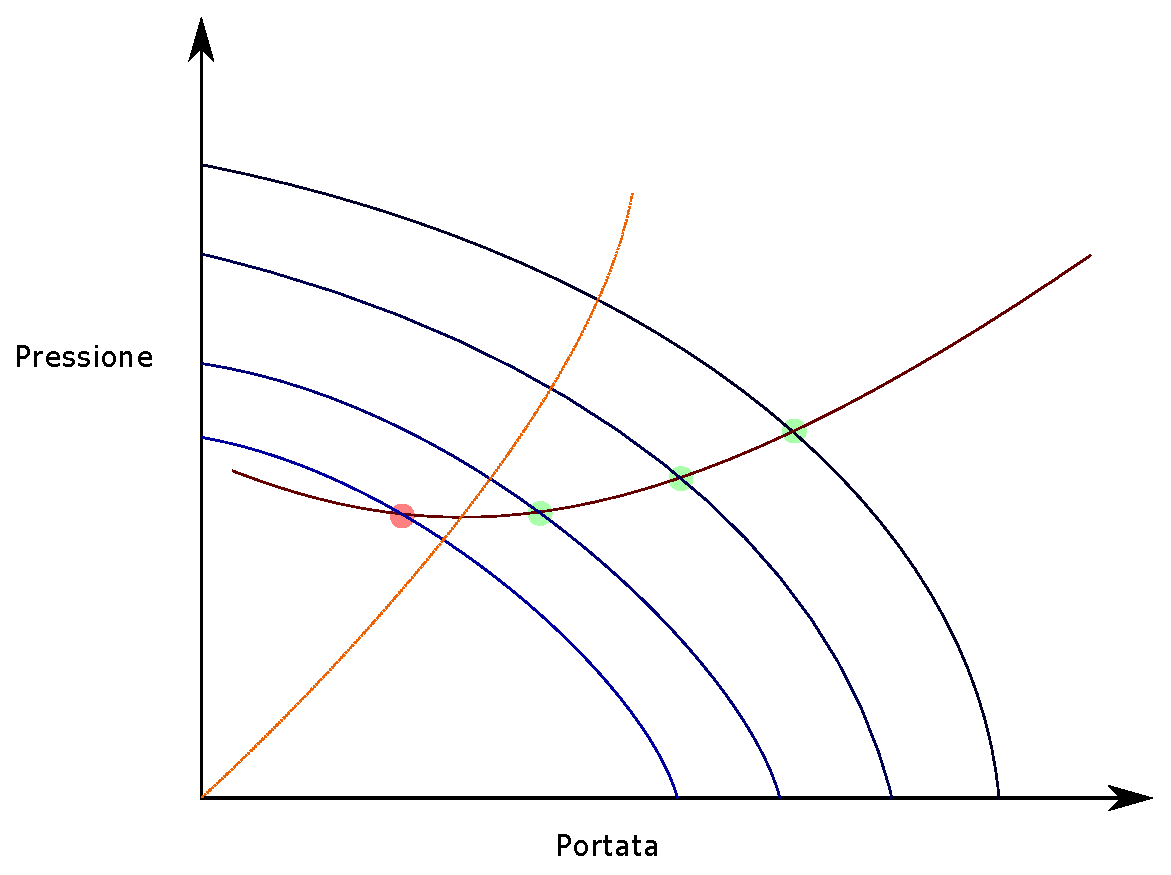
\includegraphics[width=.5\textwidth]{fig/foamer/ipr-tpr.eps}
    \caption{Analisi nodale combinata alla portata critica di trascinamento}
    \label{fig:ipr-tpr}
\end{figure}


\section[Artificial lift per GDW]{Sistemi di sollevamento artificiale per il Gas Well Deliquification}
\sectionmark{Artificial lift per GDW}
L'industria del gas utilizza numerosi metodi per la rimozione di liquidi dai pozzi. Qui di seguito sono presentati i metodi più utilizzati e ormai consolidati nel tempo con particolare attenzione agli schiumogeni a cui è dedicata una sezione a parte. \textcite{oyewole2008artificial} classifica i sistemi di sollevamento artificiale in:
\begin{itemize}
    \item \textbf{a energia del giacimento}: qui definiti  \textit{a energia interna}, i sistemi non aumentano direttamente l'energia del giacimento, bensì agiscono sui parametri che caratterizzano il trascinamento del liquido in pozzo;
    \item \textbf{a energia esterna}: sistemi a fondo pozzo che agiscono indipendentemente dall'energia residua del giacimento.
\end{itemize}
Le velocity string, i compressori, i plunger e gli schiumogeni sono sistemi di sollevamento artificiale a energia interna, pompe e iniezione di fluidi sono invece sistemi \textit{a energia esterna}.

\subsection{Velocity string}
La velocity string è praticamente un tubino di produzione con diametro inferiore rispetto a quello già presente in situ. Per produzione costante, il restringimento della sezione di produzione provoca un aumento della velocità del flusso in condotta e il superamento del valore della velocità critica. L'applicazione può avvenire su un tratto specifico del pozzo (\figref{fig:velocitystring-fixed}) oppure su tutta la lunghezza del pozzo (\figref{fig:velocitystring-long}).

\begin{figure}[htbp]
\centering
    \subfloat[][Lunghezza fissa]
    {\makebox[0.4\textwidth]{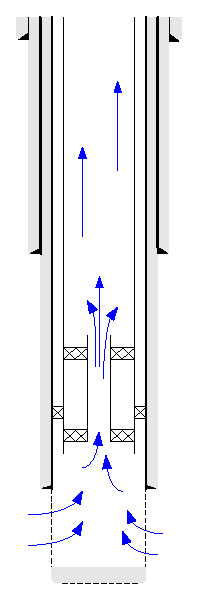
\includegraphics[width=.15\textwidth]{fig/foamer/velocitystring/velocitystring-fixed.eps}} \label{fig:velocitystring-fixed}} \quad
    \subfloat[][Su tutto il pozzo]
    {\makebox[0.4\textwidth]{\includegraphics[width=.15\textwidth]{fig/foamer/velocitystring/velocitystring-long.eps}}\label{fig:velocitystring-long}}
    \caption{Schema di applicazione della velocity string \parencite{arachman2004liquid}} 
    \label{fig:velocitystring}
\end{figure}

L'installazione della velocity string è generalmente molto economica rispetto ad altre sistemi di sollevamento artificiale, visto che l'applicazione può avvenire anche tramite \textit{coiled tubing}, prodotti tubolari continui a sezione limitata, fabbricati in lunghezza e avvolti attorno a una bobina di raccolta \parencite{international2014introduction}. Tuttavia la progettazione deve avvenire con particolare cautela, visto che il restringimento della sezione di produzione si traduce non solo in termini di aumento di velocità, ma anche di aumento delle perdite di carico per attrito. La velocity string non è considerata una soluzione definitiva per il GWD, dal momento che il dimensionamento ideale del tubino di produzione ausiliario cambia con l'evoluzione delle condizioni del giacimento.

\subsection{Compressione}
La compressione viene impiegata per diminuire la pressione a testa pozzo. La modalità di compressione può essere a opera di un singolo compressore (\figref{fig:compressore}) o di un sistema di compressori posti in superficie. 

\begin{figure}[htbp]
    \centering
    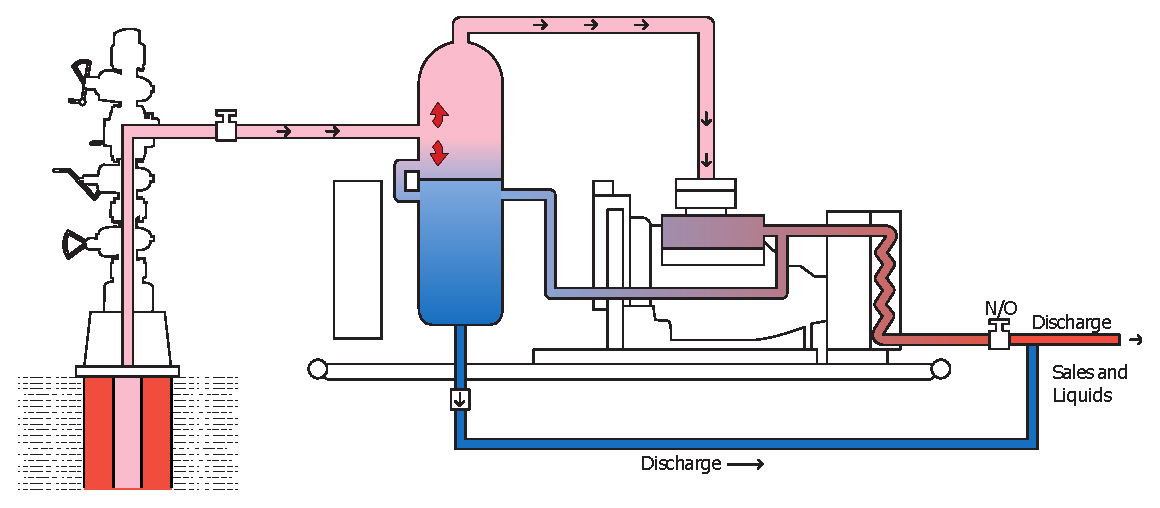
\includegraphics[width=\textwidth]{fig/foamer/compressore.eps}
    \caption{Layout semplificato del GasJack™, copressore singolo utilizzato per operazioni di compressione della testa pozzo \parencite{garner2009backside}}
    \label{fig:compressore}
\end{figure}

Una minore pressione a testa pozzo porta alla diminuzione dell'acqua proveniente da fenomeni di condensazione ma soprattutto all'aumento dell'afflusso di gas in pozzo dal giacimento. L'aumento di portata è associato all'aumento della velocità del gas, raggiungendo così valori al di sopra della velocità critica. Il dimensionamento dell'impianto di compressione si basa sulla pressione di aspirazione e la pressione di mandata, ovvero dal \textit{rapporto di compressione}. \'E importante tenere presente che una minima variazione delle pressioni di aspirazione o di mandata può aumentare in maniera significativa la potenza richiesta dal compressore. La compressione e la riduzione della pressione atesta pozzo sono generalmente le prime soluzioni impiegate per il sollevamento artificiale. L'installazione dei compressori può avvenire durante il ciclo di vita del pozzo senza evidenti segnali di \textit{liquid loading}: la diminuzione di pressione consente di lavorare in condizioni migliori, aumentando le performance generali e quindi la produzione di gas giornaliera. La compressione può anche considerarsi un sistema di sollevamento artificiale ausiliario: un compressore può interfacciarsi con altre soluzioni come agenti surfattanti, gas lift, plunger, beam pump, ESP o velocity string, aumentanto in modo significativo le performance di liquid unloading. La compressione può essere impiegata anche per avviare nuovamente un pozzo morto tramite un kick indotto dal nuovo gradiente di pressione: soluzione alquanto inusuale, l'esperienza sul campo dice che solitamente una diminuzione di pressione non è sufficiente a garantire l'energia necessaria al pozzo per poter spiazzare anche parzialmente la colonna liquida presente.

\subsection{Plunger}

I plunger sono dei dispositivi installati all'interno del pozzo capaci di rimuovere liquidi e altri agenti contaminanti meccanicamente. Il plunger è un pistone tuffante che viaggia liberamente dal fondo pozzo alla superficie, spinto da una pressione che deve essere sufficiente a trascinare sia il dispositivo che i fluidi accumulati. La produzione di gas con l'installazione di un plunger risulta discontinua, legata alla ciclicità del plunger che deve percorre in entrambe le direzioni tutta la lunghezza del pozzo. Come si può vedere nella \figref{fig:conventionalplunger} l'applicazione di un plunger in pozzo richiede l'installazione di determinati impianti di superficie (valvole) e impianti di fondo pozzo (plunger e meccanismo a molla). Una tipica installazione di plunger convenzionale è organizzata nel seguente modo:

\begin{itemize}
    \item \textbf{bumper a molla}, utile a ricevere il plunger a fondo pozzo e evitare danni dovuti all'impatto a terra;
    \item \textbf{ricevitore di superficie}, blocca il plunger una volta giunto in superficie e consente il deflusso del gas in condotta;
    \item \textbf{valvola motorizzata di superficie}, controllata elettronicamente, apre e chiude il pozzo quando necessario;
    \item \textbf{sensore elettronico di superficie}, si attiva quando il plunger giunge in superficie;
    \item \textbf{controller elettronici}, con ciclicità impostata da operatore, gestisce tutte le operazioni di produzione e registra dati in continuo.
\end{itemize}

\begin{figure}[htbp]
    \centering
    \includegraphics[width=0.6\textwidth]{fig/foamer/plunger-installation.eps}
    \caption{Tipica installazione di plunger \parencite{lea2011gas}}
    \label{fig:plunger-installation}
\end{figure}

Come già detto, l'applicazione di un plunger convenzionale trasforma la produzione da continua a ciclica, caratterizzata quindi da \textit{shut-in} programmati per far tornare il plunger a fondo pozzo e permettere al pozzo, in caso di bisogno, di raggiungere una pressione sufficiente tale da poter trascinare il plunger assieme alla colonna di fluido presente. La \figref{fig:conventionalplunger} mostra un generico ciclo di produzione di un plunger convenzionale:
\begin{enumerate}
    \item[a)] plunger a fondo pozzo con liquido al di sopra, valvola di superficie chiusa;
    \item[b)] apertura della valvola di superficie e risalita del plunger assieme alla colonna liquida;
    \item[c)] fase produttiva del pozzo in assenza di cadute di pressione dovute a liquid loading;
    \item[d)] riaccumulo di fluido a fondo pozzo;
    \item[e)] chiusura del pozzo e discesa del plunger a fondo pozzo.
\end{enumerate}

\begin{figure}[htbp]
    \centering
    \subfloat[][]
    {\centering \includegraphics[height=.3\textheight]{fig/foamer/plunger-conventional/conventionalplunger-A.eps}} \label{fig:plunger-conventional-A} \qquad \qquad
    \subfloat[][]
    {\centering \includegraphics[height=.3\textheight]{fig/foamer/plunger-conventional/conventionalplunger-B.eps} \label{fig:plunger-conventional-B}}  \qquad \qquad
    \subfloat[][]
    {\centering \includegraphics[height=.3\textheight]{fig/foamer/plunger-conventional/conventionalplunger-C.eps} \label{fig:plunger-conventional-C}} \qquad \qquad
    \subfloat[][]
    {\centering \includegraphics[height=.3\textheight]{fig/foamer/plunger-conventional/conventionalplunger-D.eps} \label{fig:plunger-conventional-D}} \qquad \qquad
    \subfloat[][]
    {\centering \includegraphics[height=.3\textheight]{fig/foamer/plunger-conventional/conventionalplunger-E.eps} \label{fig:plunger-conventional-E} }
    \caption{Ciclo di un plunger convenzionale}
    \label{fig:conventionalplunger}
\end{figure}

In commercio esistono varie tipologie di plunger e variano a seconda della geometria e degli inserti installati sulla superficie esterna (e.g. spazzole per la pulizia del tubino di produzione). Negli ultimi anni sono nati nuovi sistemi definiti a ciclo libero o in continuo, che permettono la discesa del plunger senza interrompere la produzione. Numerosi sono i brevetti e i prodotti che offrono plunger-lift in continuo: possono essere dotati di una valvola interna (e.g. Weatherford RapidFlo™, FB FreeCycle™ o McClain™) oppure a due pezzi (e.g. Peacemaker™, composto da una sfera e un manicotto). La \figref{fig:plunger} mostra alcune tipologie di plunger presenti sul mercato.\\
L'applicazione di plunger in pozzo per il sollevamento artificiale richiede un investimento iniziale relativamente basso, ma dei costi operativi che possono incidere col tempo e portare a un aumento imprevisto del costo di produzione del gas. Gli investimenti iniziali indiretti possono però incidere fortemente sulla scelta del plunger: la variazione dei volumi di gas e liquido rende necessaria una nuova valutazione circa il dimensionamento degl impianti di trattamento a valle del pozzo, i costi iniziali possono essere quindi legati per esempio all'installazione di un nuovo separatore.

\begin{figure}[htbp]
\centering
    \subfloat[][A spirale]
    {\makebox[0.2\textwidth]{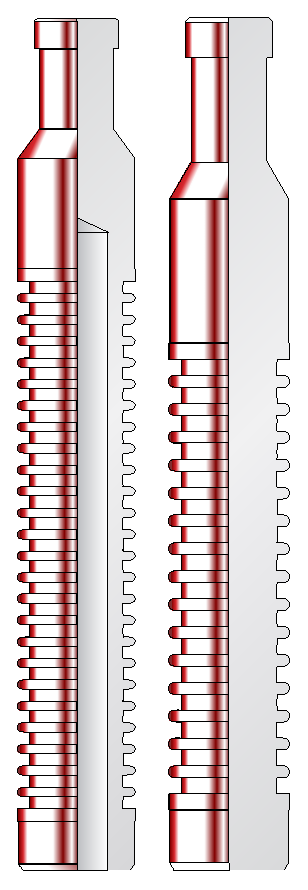
\includegraphics[height=.25\textheight]{fig/foamer/plunger/plunger-spiral.eps}} \label{fig:plunger-spiral}} \quad
    \subfloat[][T-pad]
    {\makebox[0.2\textwidth]{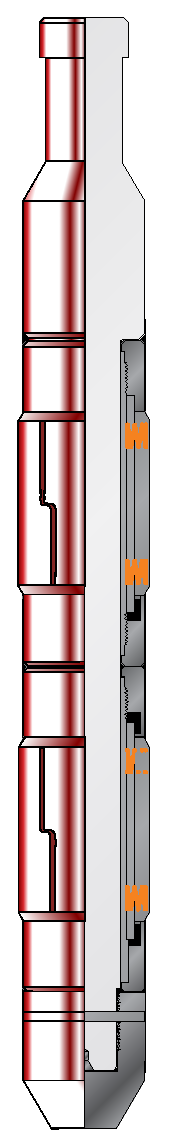
\includegraphics[height=.25\textheight]{fig/foamer/plunger/plunger-tpad.eps}} \label{fig:plunger-tpad}}  \quad
    \subfloat[][A spazzole fisse]
    {\makebox[0.2\textwidth]{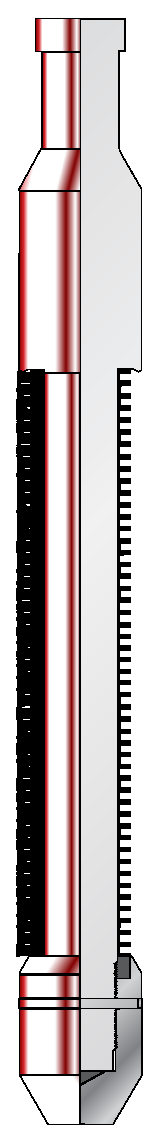
\includegraphics[height=.25\textheight]{fig/foamer/plunger/plunger-fixedbrush.eps}} \label{fig:plunger-fixedbrush}} \quad
    \subfloat[][RapidFlo™]
    {\makebox[0.25\textwidth]{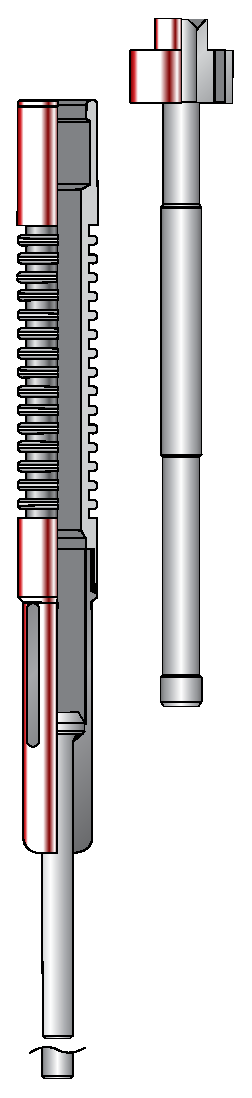
\includegraphics[height=.25\textheight]{fig/foamer/plunger/plunger-rapidflo.eps}} \label{fig:plunger-rapidflo} }
\caption{Principali tipologie di plunger proposte da Weatherford \parencite{weatherford2008brochure}}
\label{fig:plunger}
\end{figure}

\subsection[Altri sistemi per GWD]{Altri sistemi di sollevamento artificiale per deliquification}
Alcune tecnologie per l'attenuazione del battente idrostatico in pozzo nascono da applicazioni pensate in origine per il sollevamento artificiale di giacimenti a olio. Questi sistemi sono stati riadattati per il trascinamento dell'acqua a fondo pozzo o per agevolare l'afflusso del gas in pozzo. I sistemi presentati nel paragrafo corrente sono tutti a energia esterna.
\paragraph{Gas lift}
Il gas lift per dewatering consiste nell'iniezione di gas da una fonte esterna al pozzo a una certa profondità. Nel campo dell'olio il gas iniettato a fondo pozzo diminuisce la densità dell'olio, facilitando così il flusso in condotta. In questo caso viene fatto fluire gas a fondo pozzo sia per diminuire la densità della colonna idrostatica, sia per aumentare la produzione di gas effettiva e quindi l'efficacia di trascinamento della colonna idrostatica da parte della corrente gassosa. Questo sistema gode il vantaggio di non provocare significative variazioni alle conduzioni di produttività  del pozzo e riesce a lavorare anche in perforazioni deviate. L'applicazione purtroppo dipende fortemente dalla presenza di una sorgente di gas ad alta pressione, rappresentata da un pozzo nella zona limitrofe o l'installazione di un compressore, a cui però sono associati alti costi operativi. Per di più il tubino di produzione deve essere progettato per sopportare l'aumento di pressione che si ha in condotta e l'impiego di gas ad alta pressione può portare facilmente a problemi di congelamento e creazione di idrati.
\paragraph{Sistemi di pompaggio}
Le pompe petrolifere o a cavalletto (\textit{Beam Pump} o BP, impiegate in modo massiccio per il sollevamento artificiale per giacimenti a olio, rappresentano il sistema di pompaggio più comune anche nel GWD. Generalmente i sistemi di pompaggio spingono la colonna idrostatica lungo il tubino di produzione (o un tubino ausiliario, come un coiled tubing installato a posteriori) e il gas prodotto viene fatto fluire nell'annulus. Altri sistemi di pompe utilizzate anche in questo campo sono le pompe elettriche sommerse (\textit{Electrical Submersible Pump} o  ESP), pompe a cavità progressiva (\textit{Progressing Cavity Pump} o PCP) e pompe idrauliche (a pistone o \textit{jet pump}). Le pompe vengono generalmente impiegate quando la pressione a fondo pozzo è relativamente bassa e quando il rapporto gas/liquido non è sufficiente da garantire lo spiazzamento della colonna idrostatica tramite i sistemi a energia interna. Le pompe non possono operare in presenza di gas, perciò vanno opportunamente collocate al di sotto degli spari, in modo da ottenere una buona separazione del liquido dal gas. La vita media delle pompe dipende fortemente dagli agenti di erosione, è importante capire se la produzione di liquidi e gas comporta anche la produzione di gas

\section{Schiumogeni}
L'impiego di schiumogeni nell'industria petrolifera è vario e ormai consolidato nel tempo. Come visibile in \tabref{tab:surfactantapplications} i tensioattivi sono impiegati in tutte le fasi di recupero del greggio e nell'industria di processo, dalle perforazioni, iniezioni in giacimento, produzione, al trasporto in condotta onshore e offshore.

\begin{table}[htbp]
    \small
    \centering
    \caption{Alcuni esempi di applicazioni di tensioattivi nell'industria petrolifera \parencite{schramm2006emulsions}}
    \label{tab:surfactantapplications}
\begin{tabular}{p{.8\textwidth}p{.1\textwidth}}
\hline
{\bf Applicazione}                                                         & {\textbf{Fasi}\footnote{Si riferisce alle dispersioni di foamer in fase acqua (\textit{water}, W), fase olio (O), fase gas (G) e fase solida (S)}}           \\ \hline
Fluidi di perforazione con schiume                                         & G/W                    \\
Fluidi di stimolazione e fratturazione con schiume                         & G/W                    \\
Fluidi acidificanti con schiume                                            & G/W                    \\
Recupero di olio freddo e pesante tramite schiume                          & G/O                    \\
Schiume di processo della flottazione dell'olio                            & G/O                    \\
Schiume antincendio                                                        & G/W                    \\
Emulsioni per olio pesante in condotta                                     & O/W                    \\
Emulsioni per la stimolazione pozzo                                        & O/W                    \\
Flottazione di miscele a olio e sabbie bituminose                          & O/W                    \\
Fluidi di perforazione emulsionati (fanghi a base olio)                    & W/O                    \\
Emulsione di catrame e bitumi                                              & O/W                    \\
Emulsioni in situ per EOR                                                  & O/W                    \\
Emulsione di carburanti di trasporto (70\% olio pesante)                   & O/W                    \\
Schiume per il controllo della mobilità del gas                            & G/W                    \\
Sospensioni per fluidi (fanghi) di perforazione                            & S/W                    \\
Sospensioni per fratturazione idraulica e stimolazione del pozzo           & S/W                    \\
Impasti cementizi in pozzo                                                 & S/W                    \\
Solidi di produzione a testa pozzo nel recupero primario dell'olio pesante & S/W                    \\ \hline
\end{tabular}
\end{table}

I tensioattivi sono utilizzati anche in pozzo per mitigare i fenomeni di liquid loading e la tecnica ha ormai acquisito notevole importanza nel GWD. La Nederlandse Aardolie Maatschappij (NAM), compagnia petrolifera olandese, 
ha cominciato a impiegare tensioattivi o \textit{foamer} nei suoi campi a gas nell'ottobre 2003  e dopo soli due anni questo sistema è risultato altamente competitivo rispetto agli altri sistemi per il GWD \parencite{wittfeld2015foam}. 

\subsection{Tensioattivi}
I tensioattivi, surfactanti o agenti attivi di superficie sono composti organici composti al massimo da un gruppo, testa, liofilo e un gruppo, coda, liofobico \figref{fig:sls}. Si parla di testa idrofila e coda idrofoba se il solvente nel quale deve essere utilizzato il tensioattivo è acqua o a base acqua. In termini chimico-fisici la struttura di un surfactante contiene un gruppo polare e da un gruppo apolare.

\begin{figure}[htbp]
    \centering
    \includegraphics[width=.5\textwidth]{fig/foamer/sls.eps}
    \caption{Laurilsolfato di sodio, tensioattivo anionico utilizzato in molte famiglie di prodotti. La catena a 12 atomi di carbonio rappresenta il gruppo apolare (in blu) mentre il gruppo solfato associato allo ione sodio rappresenta il gruppo polare (in rosso).}
    \label{fig:sls}
\end{figure}

I surfactanti sono classificati in base alla carica del gruppo polare (\figref{fig:surfactants-classification}):
\begin{itemize}
    \item \textbf{anionici}: sali (\ce{Na+}) costituiti da lunghe catene con atomi di carbonio che terminano con un gruppo carbossilato (\ce{COO-})  o solfonato (\ce{SO3-}, \ce{SO4-});
    \item \textbf{cationici}: sali (\ce{Cl-}, \ce{Br-}) di cui è importante la parte positiva, costituita da lunghe catene di atomi di carbonio terminanti con un gruppo ammonico;
    \item \textbf{non ionici}: alcoli a lunga catena, come i derivati poliossietilenici degli acidi grassi;
    \item \textbf{anfoteri} o \textbf{zwitterionici}: tensioattivi anionici in ambiente alcalino, tensiattivi cationici in ambiente acido.
\end{itemize}

\begin{figure}[htbp]
    \centering
    \subfloat[][Anionici]
    {\includegraphics[width=.45\textwidth]{fig/foamer/surfactants-classification/anionic.eps} \label{fig:anionic}} \quad
    \subfloat[][Cationici]
    {\includegraphics[width=.45\textwidth]{fig/foamer/surfactants-classification/cationic.eps} \label{fig:cationic}}  \\
    \subfloat[][Anfoterici]
    {\includegraphics[width=.45\textwidth]{fig/foamer/surfactants-classification/anphoteric.eps} \label{fig:anphoteric}}  \quad
    \subfloat[][Non ionici]
    {\includegraphics[width=.45\textwidth]{fig/foamer/surfactants-classification/nonionic.eps} \label{fig:nonionic}} 
\caption{Classificazione dei tensioattivi in base alla carica del gruppo polare}
\label{fig:surfactants-classification}
\end{figure}

Due fenomeni derivano dalla presenza di un gruppo polare e apolare all'interno della stessa molecola: adsorbimento e aggregazione.\\
Si consideri un volume d'acqua a contatto con aria dove vengono disciolti dei tensioattivi. I surfactanti, in prossimità della superficie di contatto delle due fasi, si orientano in modo tale che il gruppo polare sia adsorbito dalla fase liquida e il gruppo apolare permanga nella fase gassosa. Tale adsorbimento porta alla diminuzione dell'energia libera di Gibbs o entalpia libera, quindi alla riduzione della tensione superficiali tra le due fasi.. Allo stesso modo i tensioattivi possono diminuire la tensione superficiale di acqua a contatto con una generica fase olio o di un solido, aumentando in questo caso la bagnabilità di quest'ultimo.

Un altro modo per limitare il contatto del gruppo apolare con l'acqua è la creazione di strutture bi- o tridimensionali, capaci di racchiudere i gruppi apolari internamente e mettendo a contatto con l'acqua i gruppi polari \figref{fig:micelle}. Queste strutture sono definite micelle, sono il frutto dei fenomeni di aggregazione dei tensioattivi e possono avere forma lamellare (in questo caso i surfactanti sono molecole anfifiliche o anfifobiche, sferica o cilindrica.  Tali aggregati supramolecolari tendono a crearsi una volta superato un certo valore di concentrazione del surfactante in soluzione, definito \textit{concentrazione micellare minima}. La complessità di tali strutture dipende dalla concentrazione in acqua e dalla specie chimica dell'agente attivo di superficie.

\begin{figure}[htbp]
    \centering
    \includegraphics[width=.5\textwidth]{fig/foamer/micelle.eps}
    \caption{Sezione parziale di una micella anionica, il layer compatto negativo generato dall'orientamento del gruppo polare del tensioattivo è circondato dalla fase acqua  \parencite{attwood2012fasttrack}.}
    \label{fig:micelle}
\end{figure}



\section{Applicazioni di schiumogeni per l'attenuazione del liquid loading}
aerhheraeherh

\subsection{Schiumogeni in pozzo}
sdgrahthr
\subsection{Stick}
rtssrtjtysr
\subsubsection{Schiuma in-batch}
srtujrt
\subsubsection{Schiuma in continuo}
rtsustyuy

\section{Confronto tra le tecnologie di sollevamento artificiale per pozzi a gas}
Citare tutti i lavori di GDW 2014-2015
\clearpage{\pagestyle{empty}\cleardoublepage}
\chapter{Impianti di trattamento del gas naturale}\thispagestyle{empty}
\chaptermark{Trattamento gas naturale}
Per trattamento di gas naturale si intende l'insieme delle operazioni utili alla riduzione o abbattimento dei componenti che possono incidere sul trasporto e sull'utilizzo ultimo della risorsa. Le reti di distribuzione su larga scala prevedono delle specifiche tecniche e i trattamenti sono mirati al fine di ottenere valori che rispettino questi criteri. La produzione di gas naturale è normalmente associata alla presenza di acqua, la quale può presentarsi in forma liquida o gassosa. Il trattamento della disidratazione è fondamentale al fine di impedire la formazione di idrati, composti solidi che possono danneggiare le condotte durante il trasporto. Altri trattamenti sono legati al recupero degli idrocarburi condensati, che si manifestano al cambiare delle condizione di pressione e temperatura in superficie, e alla presenza di elementi corrosivi e elementi inerti, che possono diminuire i rendimenti del gas naturale.
Il trattamento definitivo del gas può essere preceduto da un trattamento provvisorio (\figref{fig:generaltreatment}), nel quale si riducono o si inibiscono momentaneamente gli effetti dei componenti indesiderati del gas. Solitamente si fa riferimento al trattamento provvisorio nel trasporto del gas prodotto dall'area pozzo alla centrale di trattamento.

\begin{figure}[htbp]
    \centering
    \includegraphics[width=\textwidth]{fig/impianti/generaltreatment.eps}
    \caption{Tipologie di trattamento.}
    \label{fig:generaltreatment}
\end{figure}

Nel seguente capitolo si espongono le specifiche tecniche del gas, i processi di trattamento e le relative apparecchiature e impianti.

\section{Specifiche del gas di vendita}
Il gas naturale è una miscela di idrocarburi solitamente allo stato gassoso costituita in gran parte da metano e da idrocarburi più pesanti. Altre componenti spesso presenti sono acqua, anidride carbonica, azoto, idrogeno solforato e solfati, in alcuni casi anche elio e metalli pesanti come mercurio. In \tabref{tab:ng-composition} è riportato un esempio di composizione centesimale di un gas naturale. 

\begin{table}[htbp]
    \small
    \centering
    \caption{Composizione centesimale di un gas naturale tramite cromatografia del gas \parencite{mele2012produzione}.}
    \label{tab:ng-composition}
    \begin{tabular}{p{.45\textwidth}p{.45\textwidth}}
        \hline
        {\bf Componenti}                & {\textbf{\% in volume}}       \\ \hline
        Azoto                           & {0,17}                        \\
        Anidride carbonica              & {0,02}                        \\
        Metano                          & {99,71}                       \\
        Idrogeno solforato              & {-}                           \\
        Etano                           & {0,06}                        \\
        Propano                         & {0,03}                        \\
        Iso-butano                      & {0,01}                        \\
        Neopentano                      & tracce                        \\
        Iso-pentano                     & -                             \\
        Esani                           & -                             \\
        Ottani                          & -                             \\
        Eptani                          & -                             \\ \hline
    \end{tabular}
\end{table}

Ai fini della distribuzione e vendita, il gas naturale deve rispettare parametri specifici per poter poi essere immesso nelle reti nazionali. La rete di distribuzione su larga scala non prevede alcun trattamento del gas, ma delle semplici compressioni e decompressioni a seconda delle esigenze dell'utente finale. Il gas deve essere quindi opportunamente trattato nel rispetto di tali specifiche.

\paragraph{Potere calorifico e indice di Wobbe}
Il gas naturale viene utilizzato maggiormente come combustibile e deve fornire un potere calorifico a specifica su tutto il territorio nazionale. Come parametro di riferimento si assume il potere calorifico superiore (PCS) pari a 9.100 kcal/Sm\ap{3} o 38,1 MJ/Sm\ap{3} (il PCS del gas metano puro è 9.001,6 kcal/Sm\ap{3}), con un campo di variabilità nell'ordine del ±10\%. \'E importante ricordare che il PCS di un gas naturale può raggiungere questi valori anche in presenza di gas inerti come anidride carbonica e azoto, essendo formato da idrocarburi superiori che innalzano notevolmente il potere calorifico medio.\\
A questo proposito è utile introdurre l'indice di Wobbe \(I_W\) definito come:
\[I_w = \dfrac{\textrm{PCS}}{\sqrt{\rho_s}} \label{eq:wobbe} \]
dove \(\rho_s\) è la densità specifica del gas (densità relativa rispetto a quella dell'aria). Se si prende come riferimento il metano, l'indice di Wobbe è pari a 12.094,8 kcal/Sm\ap{3} o 50.604,64 kJ/Sm\ap{3}, con una variabilità consentita del ±5\%. Nella valutazione della compatibilità di un gas per la sua immissione nella rete di distribuzione, è più corretto far riferimento all'indice di Wobbe: il campo di variazione più ristretto equivale a una minore presenza di gas inerti in miscela.

\paragraph{Punto di rugiada dell'acqua e degli idrocarburi}
Il gas non deve presentare condizioni di condensazione di acqua e/o idrocarburi in alcuna fase di trasporto e distribuzione. Le specifiche di pressione e temperatura variano a seconda delle diverse condizioni geografiche e climatiche, con queste anche i punti di rugiada (\textit{dew point}) dell'acqua e degli idrocarburi. Questi valori sono calcolabili tramite la rappresentazione del diagramma di fase relativo. Si considerano due specifiche diverse (in acqua e in idrocarburi) per i motivi seguenti:
\begin{itemize}
    \item \textbf{formazione di idrati}: si deve tenere maggiormente in considerazione la condensazione d'acqua rispetto a quella di idrocarburi a causa della formazione di idrati in condotta (trattati più avanti nel paragrafo ~\ref{section:dehidratation}). I margini operativi per la condensazione dell'acqua devono essere quindi più elevati;
    \item \textbf{andamento non univoco della saturazione rispetto alla pressione}: essendo il gas naturale una miscela multicomponente, nel definire la specifica di \textit{dew point} in idrocarburi non si fa riferimento, come in acqua, a una pressione prefissata, ma a tutto il campo i pressioni a partire da quella atmosferica. Il diagramma di fase di una miscela multifase, visibile in \figref{fig:phasediagram}, è caratterizzato dalla zona di condensazione retrograda: in questa condizione con una riduzione di pressione (a temperatura costante) gli idrocarburi condensano anziché evaporare.
\end{itemize}

\begin{figure}[htbp]
    \centering
    \includegraphics[width=.6\textwidth]{fig/impianti/phasediagram.eps}
    \caption{Diagramma di fase per una miscela multicomponente \parencite{bianco2005impiantigas}}
    \label{fig:phasediagram}
\end{figure}

\paragraph{Gas inerti (\ce{CO2} e \ce{N2})}
L'anidride carbonica (\ce{C O2}) in giacimento nasce dall'iterazione delle acque di strato con i silicati e i carbonati presenti. Raramente l'acido carbonico, composto che si forma per idratazione dell'anidride carbonica: 
\[\ce{H2O + CO2 -> H2CO3} \addtag \label{eq:acidocarbonico}\]
rappresenta un problema concreto per gli impianti di trasporto del gas naturale. Il contenuto di \ce{CO2} nel gas naturale non influenza significativamente l'indice di Wobbe, ma contribuisce all'incremento dei gas inerti totali (l'azoto \ce{N2} e appunto l'anidride carbonica). Si preferisce comunque rimuovere il \ce{CO2} (fino al raggiungimento dell'indice di Wobbe) rispetto all'azoto per la sua facilità tecnica di abbattimento. In generale si parla di volumi accettabili di \ce{CO2} attorno al 3\% con un contenuto totale di gas inerti che non deve mai superare il 6,5\%.

\paragraph{Acido solfidrico (\ce{H2S})}
L'acido solfidrico o idrogeno solforato (\ce{H2S}) è un gas incolore dall'odore caratteristico di uova in decomposizione. \'E presente naturalmente nel petrolio e nel gas naturale e rappresenta uno dei sottoprodotti della decomposizione di proteine contenenti zolfo e dalla riduzione diretta di solfati (\ce{SO4^2-}) da parte di batteri, funghi e attinomiceti presenti in ambiente anossico. L'\ce{H2S} è la principale causa di corrosione nella produzione di gas naturale, è altamente tossico e, per certe concentrazioni, anche mortale. Il contenuto massimo accettato è molto basso: Snam Rete Gas richiede un contenuto massimo di 6,6 mg/Sm\ap{3}.

\paragraph{Zolfo totale}
L'abbattimento dello zolfo totale nel gas naturale è legato più a questioni ambientali che a questioni di sicurezza. Il contenuto di zolfo totale massimo richiesto da Snam Rete Gas è di 150 mg/Sm\ap{3}, con un valore massimo di zolfo da mercaptani 15,5 mg/Sm\ap{3}. La rimozione dei mercaptani avviene tramite impianti che differiscono da quelli utilizzati per la rimozione di acido solfidrico e altri acidi.

\paragraph{Solidi sospesi}
I solidi sospesi vengono normalmente abbattuti durante i processi di separazione dei liquidi dal gas. Solo in casi particolari il gas naturale viene posto a processi di filtrazione meccanica.

\begin{table}[htbp]
    \small
    \centering
    \caption{Parametri di controllo della qualità richiesti dalla Snam Rete Gas \parencite{snam2015codice}.}
    \label{tab:ng-specifiche}
    \begin{tabular}{p{.4\textwidth}p{.2\textwidth}p{.23\textwidth}}
        \hline 
        {\bf Parametri} & \multicolumn{1}{l}{{\bf Valori consentiti}} & {\bf Unità di misura} \\ \hline \hline
        Potere Calorifico Superiore & 34,95 ÷45,28 & MJ/Sm\ap{3} \\\hline
        Indice di Wobbe & 47,31÷52.33 & MJ/Sm\ap{3} \\\hline
        Densità relativa & 0.5548÷0,8 &  \\\hline
        Ossigeno & \(\leq\) 0,6 & \% mol \\\hline
        Punto di Rugiada dell'acqua (p=7 MPa) & \(\leq\) -5 & °C \\\hline
        Punto di Rugiada degli idrocarburi (p=0,1÷7 MPa) & \(\leq\) 0 & °C \\\hline
        Temperatura max & \textless 50 & °C \\\hline
        Solfuro di idrogeno & \(\leq\) 6,6 & mg/Sm\ap{3} \\\hline
        Zolfo da mercaptani & \(\leq\) 15,5 & mg/Sm\ap{3} \\\hline
        Zolfo Totale & \(\leq\) 150 & mg/Sm\ap{3} \\ \hline
    \end{tabular}
\end{table}

\section{Separazione gas-liquido}
La dinamica delle particelle disperse in un fluido studia i fenomeni di sedimentazione di gocce di liquido in un gas applicando gli stessi principi della separazione per gravità liquido-liquido. Il calcolo della velocità terminale \(w_t\) viene effettuato in base al bilancio statico delle forze che agiscono sulla singola particella, condizione nella quale la velocità è costante. Nel caso di particelle sferiche indeformabili di raggio \(D_p\)
\[w_t=\sqrt{\dfrac{4 \; g \; D_p(\rho_p-\rho_f)}{3 \; C_D \; \rho_l}} \addtag \label{eq:velterminale}\]
dove \(g\) è l'accelerazione di gravita, \(\rho_p\) e \(\rho_f\) sono la densità rispettivamente della particella e del fluido disperdente, \(C_D\) è definito coefficiente di galleggiamento o \textit{drag coefficient}. Nel caso di separazione per gravità liquido-liquido e condizioni di moto laminare, quindi per bassi valori del numero di Reynolds \(R_e\), la \eqref{eq:velterminale} assume la forma della legge di Stoke:
\[w_t= \dfrac{(\rho_p-\rho_f)}{18\mu} \; D_p^2\; g \addtag \label{eq:stoke}\]
Per quanto riguarda particelle fluide immerse in un gas la condizione di moto laminare non è rispettata, a causa dei bassi valori della viscosità del gas quindi dell'alto valore del numero di Reynolds. In questo caso il calcolo del coefficiente di galleggiamento è effettuato tramite modelli sperimentali e calcolo per tentativi (\textit{trial and error}). La separazione per gravità è un processo grossolano che permette l'abbattimento di particelle nell'ordine di \SI{250}{\um} o di poco inferiore. Gli abbattitori (anche \textit{knockout} o KOD, \textit{Knock-Down Drum}) sono particolari separatori che agiscono per semplice gravità, utili per eliminare o solo l'acqua liquida o tutto il fluido trascinato dal gas. Sono generalmente collocati a monte di impianti di separazione meccanica a bassa temperatura (par. ~\ref{subsection:lts}) o a protezione di una fiaccola. Il dimensionamento dei KOD è basato sul bilancio tra tempo di ritenzione e tempo di decantazione delle particelle liquide in flusso gassoso.
Nei casi in cui si vogliano ottenere delle migliori performance di abbattimento dei liquidi si deve ricorrere a unità snebbianti che facilitino la coalescenza delle gocce e favoriscano l'abbattimento di gocce con diametro superiore ai \SI{10}{um}. Una delle unità snebbianti più comunemente utilizzate è il pacco rete (\textit{wire mesh pad}), inserito perpendicolarmente al flusso del gas. L'equazione che determina la velocità massima nella materassina snebbiante (\textit{mist eliminator}) è:
\[ w_t=K \sqrt{\dfrac{\rho_p-\rho_f}{\rho_f}} \addtag \label{eq:rete}\]
dove costante K varia in base al separatore e alla pressione operativa.\\
Nel campo della separazione di liquidi dal gas sono molto utilizzati anche i cicloni e i pacchi vani. I cicloni sono unità di coalescenza che sfruttano l'effetto centrifugo ottenuto tramite il movimento circolare del gas, con abbattimento delle particelle liquide fino ai \SI{3}{mu}. I pacchi di vani sono elementi coalescenti molto utilizzati anche nel trattamento dell'olio e sfruttano l'"effetto chicane" che si instaura nel flusso. Queste due unità di coalescenza sono preferite per il trattamento di gas caratterizzato da un notevole contenuto di solidi, come cristalli di paraffina separatisi dalla fase liquido in condizioni di bassa temperatura.

\section{Disidratazione e degasolinaggio} \label{section:dehidratation}
La variazione delle condizioni operative può dar luogo a fenomeni di condensazione di idrocarburi e/o acqua a partire da una miscela di idrocarburi allo stato gassoso. Quando in una corrente di gas naturale si ha la formazione di acqua libera, per determinate condizioni di flusso possono formarsi dei composti solidi detti idrati.
Il termine "idrato" è un termine generico per intendere nello specifico i composti di inclusione o clatrati (dal latino \textit{clauthratus}, ingabbiato), strutture molecolari in cui un tipo di molecole avvolge un altro tipo di molecole. Le prime sono dette molecole ospitanti mentre le altre molecole ospiti. Per gli idrati di gas naturale le molecole ospitanti sono le molecole di acqua, mentre le molecole ospiti sono le molecole costituenti il gas naturale. La particolare conformazione è stabile in fase solida, dove le molecole ospitanti formano un reticolo cristallino al cui interno si generano della cavità in cui si posizionano le molecole di gas. 
A differenza del ghiaccio, la formazione degli idrati è fortemente dipendente dalle condizioni di pressione: maggiore è la pressione parziale del gas (quindi la concentrazione di molecole ospiti), maggiore è la temperatura di formazione degli idrati. La tendenza a formare idrati negli idrocarburi leggeri aumenta con il peso molecolare dell'idrocarburo e la presenza di anidride carbonica (\ce{CO2}) e solfuro di idrogeno (\ce{H2S}). 
In generale, affinché gli idrati si possano formare è necessario che si instaurino le seguenti condizioni:
\begin{itemize}
    \item presenza acqua allo stato liquido;
    \item presenza di idrocarburi;
    \item moto turbolento;
    \item pressione e temperatura.
\end{itemize}
Sono stati sviluppati dei diagrammi che consentono di prevedere la formazione di idrati a determinate condizioni di pressione e temperatura, in funzione alla densità o peso molecolare medio del gas \figref{fig:formazioneidrati}.
\begin{figure}[htbp]
    \centering
    \includegraphics[width=.5\textwidth]{fig/impianti/formazioneidrati.eps}
    \caption{Diagramma della formazione degli idrati in funzione di temperatura e pressione \parencite{bianco2005impiantigas}.}
    \label{fig:formazioneidrati}
\end{figure}
Gli idrati possono formarsi all'interno delle singole condotte o concentrate su un collettore e possono danneggiare l'impianto in numerosi modi. L'occlusione parziale o totale della condotta porta a un aumento incontrollato della pressione a monte del tappo di idrati con conseguente rottura della linea o per squarciamento della stessa o per impatto in corrispondenza di una curva (\figref{fig:idrati1}). Il tappo di idrati soggetto a riscaldamento localizzato può espandersi in modo incontrollato, portando all'inevitabile rottura della condotta (\figref{fig:idrati2}). Con l'interruzione di produzione a opera di una valvola, se la velocità del tappo è sufficientemente elevata, la quantità di moto degli idrati può produrre pressioni così elevate da far scoppiare la linea (\figref{fig:idrati3}).

\begin{figure}[htbp]
    \centering
    \subfloat[][Rottura per impatto di idrati su elemento curvo della condotta.]
    {
\includegraphics[width=.45\textwidth]{fig/impianti/idrati/idrati2.eps}  \label{fig:idrati1}} \qquad
    \subfloat[][Rottura per riscaldamento e espansione incontrollata.]
    {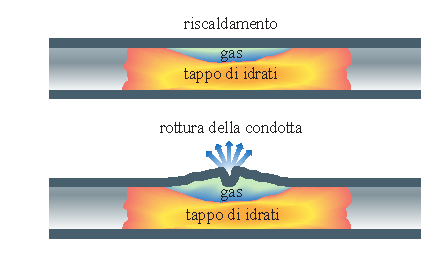
\includegraphics[width=.45\textwidth]{fig/impianti/idrati/idrati1.eps} \label{fig:idrati2}} \\
    \subfloat[][Rottura per inerzia del tappo di idrati.]
    {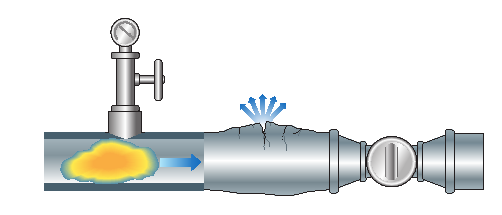
\includegraphics[width=.45\textwidth]{fig/impianti/idrati/idrati3.eps} \label{fig:idrati3}} 
\caption{Danni in condotta creati dalla formazione di idrati \parencite{borghi2005idrati}.}
\label{fig:idrati}
\end{figure}

Si inibisce la formazione di idrati in via temporanea aumentando la temperatura di trasporto del gas o tramite l'impiego di inibitori chimici, in via del tutto definitiva con la completa disidratazione chimica.

\subsection{Inibizione chimica}
Gli inibitori vengono utilizzati per brevi tratti di linea, come i collegamenti tra le aree pozzo e le centrali di trattamento del gas naturale. Gli inibitori di idrati sono composti ad alta igroscopicità e possono agire in fase sia gassosa che liquida come l'alcol metilico (\ce{CH3-OH}), sia in fase solo liquida come il glicol monoetilenico o EG(\ce{C2H6O2}) e dietilenico o DEG(\ce{C4H10O3}). Il glicol è preferito all'alcol metilenico per la minore volatilità e infiammabilità.
Gli inibitori agiscono sul flusso gassoso in modo da abbassare il punto di congelamento spostando la formazione degli idrati verso valori più bassi di temperatura. La quantità o la concentrazione di glicol da iniettare è legata alle condizioni operative con cui si intende trasportare il gas naturale. La \figref{fig:inibizioneidrati} mostra l'abbassamento della temperature relativa alla curva di formazione degli idrati in funzione della concentrazione di EG (glicol etilenico o etilenglicol) disciolto in acqua.

\begin{figure}[htbp]
    \centering
    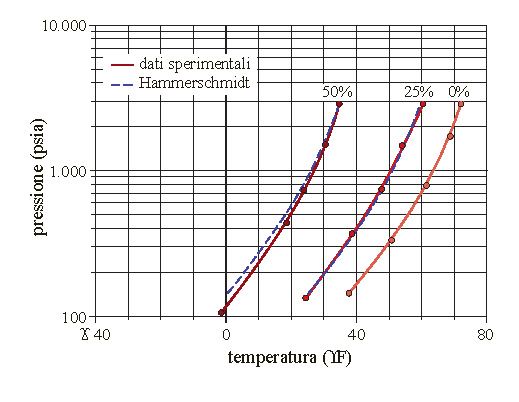
\includegraphics[width=.5\textwidth]{fig/impianti/inibizioneidrati.eps}
    \caption{Inibizione degli idrati tramite glicol etilenico \parencite{bianco2005impiantigas}.}
    \label{fig:inibizioneidrati}
\end{figure}

La rigenerazione del glicol, diluito in acqua all'arrivo della condotta, avviene tramite ebollizione dell'acqua in condensa, solitamente alla temperatura di 130°C.
Mentre in passato l'inibizione degli idrati era un sistema impiegato spesso per il trasporto del gas naturale dalle aree pozzo alla centrale di trattamento, oggi si preferisce installare un sistema di disidratazione in prossimità del sito di produzione, soprattutto quando le condotte sono di notevole lunghezza.

\subsection{Disidratazione per raffreddamento} \label{subsection:lts}
Uno dei sistemi più semplici per la disidratazione di un gas consiste nel raffreddamento del gas stesso. La temperatura finale del trattamento deve coincidere con il punto di rugiada che si vuole ottenere. La disidratazione per raffreddamento, condizionamento a freddo o separazione a bassa temperatura (\textit{Low-Temperature Separation}, LTS) si ottiene sfruttando l'effetto Joule-Thomson: grazie alla semplice espansione, la corrente gassosa riesce a diminuire la propria temperatura senza l'ausilio di energia esterna. L'intero processo viene ottimizzato tramite uno scambio termico carica-effluente a opera di uno scambiatore gas-gas, tale da sfruttare le temperature raggiunte nel processo come punti di pre- e post-trattamento del gas naturale. Gli impianti LTS richiedono pozzi a gas ad alta pressione che garantiscano un sufficiente salto entalpico. Le basse temperature permettono di ottenere un sensibile abbassamento del punto di rugiada del gas e un maggiore recupero di condensato rispetto ai separatori tradizionali. \\
Gli impianti di separazione a bassa temperatura (\figref{fig:lts}) si basano su due elementi di processo fondamentali:
\begin{itemize}
    \item separatore a bassa temperatura;
    \item scambiatore di calore.
\end{itemize}

\begin{figure}[htbp]
    \centering
    \includegraphics[width=.7\textwidth]{fig/impianti/lts.eps}
    \caption{Condizionamento del gas tramite separatore a bassa temperatura \parencite{bianco2005impiantigas}.}
    \label{fig:lts}
\end{figure}

Il separatore a bassa temperatura, anche detto separatore a freddo o a espansione, rappresenta il fulcro dell'impianto. Il gas viene immesso nella parte superiore del separatore tramite una duse. L'espansione del gas provocato dalla duse porta a una diminuzione repentina della temperatura del flusso con la condensazione di acqua. L'acqua, precipitando verso il basso, forma degli idrati che si raccolgono anche essi nella sezione inferiore per gravità. I liquidi e gli idrati vengono raccolti e scaldati tramite il gas in arrivo dal pozzo tramite una serpentina immersa. Questo riscaldamento viene effettuato per abbattere gli idrati e far rievaporare nuovamente i componenti leggeri come metano e etano. Il rendimento del processo dipende fortemente dalla temperatura finale raggiunta, perciò si consiglia di isolare i separatori a bassa temperatura per aumentare le performance di separazione per condensazione.
Lo scambiatore di calore gas-gas svolge una duplice funzione: provvede al preraffreddamento del gas in ingresso all'impianto di condensazione e al riscaldamento del gas in uscita riducendo al minimo la formazione di idrati. \\
L'unità di separazione a freddo può essere dotata di iniezione di inibitori al fine di abbassare ulteriormente la possibilità che si possano creare degli idrati al proprio interno. L'iniezione avviene a valle dell'espansione del gas e il sistema viene munito di un'unità di rigenerazione del glicol associato all'acqua in uscita.\\
Se le pressioni di arrivo del gas non sono sufficienti affinché l'espansione raggiunga temperature desiderate, l'impianto può essere aiutato da un ciclo di refrigerazione esterno a freon o propano. In questo caso si parlerà di disidratazione per raffreddamento con refrigerante o CRC (\textit{Compression Refrigeration Cycle}) e la temperatura di separazione viene ottenuta con uno scambiatore (\textit{chiller}) in cui il fluido refrigerante evapora a bassa temperatura e sottrae calore al gas da trattare. Le altre componenti dell'unità di trattamento non differisco dall'impianto LTS fin qui descritto.\\
Gli impianti di separazione a freddo sono impiegati non solo per la disidratazione del gas ma anche per il recupero degli idrocarburi superiori e pesanti in fase gassosa. Per la trattazione specifica si rimanda al paragrafo ~\ref{subsection:gasolina}.


\subsection{Disidratazione mediante assorbimento con glicol}
In questo tipo di disidratazione la tipologia di glicol più utilizzata è il trietilenico o TEG (\ce{C6H14O4}), anche se in alcuni casi può essere impiegato il DEG o l'EG. Il TEG è preferito agli altri per la più alta temperatura di decomposizione, importante ai fini della rigenerazione del glicol. La \figref{fig:disidratazioneglicol} mostra uno schema semplificato di impianto per la disidratazione con glicol.
\begin{figure}[htbp]
    \centering
    \includegraphics[width=.7\textwidth]{fig/impianti/deidratazioneglicol.eps}
    \caption{Schema semplificato di disidratazione con glicol \parencite{bianco2005impiantigas}.}
    \label{fig:disidratazioneglicol}
\end{figure}
Una corrente di TEG concentrato viene iniettata nella parte superiore della colonna di disidratazione, al fondo della quale viene fatto confluire il gas naturale da trattare. Il contatto col gas del glicol, altamente igroscopico, con più stadi di equilibrio in controcorrente porta alla disidratazione della corrente gassosa in uscita alla testa della colonna di assorbimento. Il TEG umido, cioè diluito in acqua, giunge al fondo della colonna e viene raccolto e inviato all'impianto di rigenerazione. Il recupero avviene tramite distillazione della soluzione.
La colonna di rigenerazione è divisa in due parti dalla sezione di alimentazione del glicol, dove la parte superiore è definita di rettifica, quella inferiore di arricchimento. Il TEG condensato viene preriscaldato tramite serpentina installata all'interno della colonna di rigenerazione, che funge da condensatore per abbattere le perdite di TEG. \\
Prima dell'immissione il TEG ricco viene convogliato in una camera di flash o \textit{flash drum}, nel quale i gas associati vengono recuperati tramite espansione a bassa pressione alla testa del separatore. \\
Dopo un eventuale passaggio tramite filtri a maglia e a carboni attivi, Il TEG ricco giunge alla colonna di rigenerazione, riscaldata tramite ribollitore di fondo solitamente di tipo \textit{kettle}. La temperatura del bollitore varia in funzione del tipo di glicol utilizzato: nel caso di utilizzo di TEG la temperatura è leggermente superiore ai 200°C in quanto ai 207°C il TEG tende a degradare, con DEG e EG le temperature operative scendono in quanto degradano attorno ai 165°C.\\
Per il riscaldamento si possono utilizzare vari sistemi (come tubi di fiamma e tubi di fumo immessi nel bagno da scaldare, fascio tubiero tradizionale, riscaldatore elettrico a resistenze corazzate, olio caldo (\textit{hot oil}), l'installazione deve avere comunque un occhio di riguardo sulla distribuzione della temperatura, ovvero il riscaldamento deve essere uniforme su tutta la superficie della camera di rigenerazione. \\
Il TEG rigenerato cede gran parte del calore passando nello scambiatore carica-effluente, viene pompato alla pressione di assorbimento e raffreddato alla testa della colonna di assorbimento.\\
Il trattamento continuo di disidratazione per glicol risulta essere molto semplice e il sistema di rigenerazione permette di raggiungere degli ottimi valori di concentrazione finale di TEG (solitamente attorno  al 98\%). Se si vogliono ottenere concentrazioni maggiori, occorrono dei processi di rigenerazione spinta con le quali i valori sono prossimi al 99,98\%. I processi di rigenerazione spinta più comuni sono l'installazione di colonna di \textit{stripping} con gas (\textit{dryer}), la rigenerazione sottovuoto (pressioni prossime a 0,1 bar) o i sisemi Drizo (utilizzo di gas di \textit{stripping} ottenuto vaporizzando composti liquidi mediante un adeguato serpentino di riscaldamento).

\subsection{Disidratazione mediante adsorbimento con setacci molecolari}
Nel caso in cui si voglia avere una disidratazione pressoché totale si può disidratare la corrente gassosa tramite adsorbimento a letto solido. L'acqua e alcuni inquinanti polari come \ce{CO2}, \ce{H2S} e mercaptani sono adsorbiti da un zeoliti, cristalli altamente porosi appartenenti alla classe degli allumninosilicati. Essi hanno caratteristiche del tutto simili alle argille naturali: agiscono come un filtro molecolare (\textit{molecular sieve}), lasciando passare il gas e trattenendo le molecole polari. I cristalli di zeolite sono mischiati a dei leganti a base argillosa per ottenere i letti molecolari. L'adsorbimento è reversibile e i cristalli di zeolite possono essere rigenerati: le molecole adsorbite possono essere rilasciate in condizioni di alta temperatura o basse pressioni \parencite{grace2010techinf}. \\
Un tipico impianto di disidratazione è composto da due o più colonne di adsorbimento a setacci molecolari (solitamente tre, due in funzione e una in rigenerazione) e da un riscaldatore di gas di rigenerazione. L'adsorbimento di acqua si ottiene facendo confluire la corrente gassosa dall'alto verso il basso (\textit{down flow}) e il gas secco, in uscita dalla parte inferiore, viene immesso direttamente in rete. La rigenerazione dei setacci molecolari avviene tramite \textit{stripping}: il gas caldo di rigenerazione viene fatto fluire in senso opposto rispetto a quello di adsorbimento (\textit{up flow)}. L'aumento di temperatura consente la rimozione delle molecole polari adsorbite dai cristalli di zeolite e si associano alla corrente gassosa calda. Il gas di rigenerazione in uscita viene raffreddato e l'acqua viene separata per condensazione, mentre il gas viene riciclato verso i letti molecolari in funzione.\\
I setacci molecolari sono impiegati non solo per la disidratazione del gas ma anche per prodotti liquidi leggeri come GPL e condensati recuperati tramite LTS.

\begin{figure}[htbp]
    \centering
    \includegraphics[width=.7\textwidth]{fig/impianti/molecularsieve.eps}
    \caption{Schema di disidratazione a due letti \parencite{bianco2005impiantigas}.}
    \label{fig:molecularsieve}
\end{figure}

\subsection{Degasolinaggio} \label{subsection:gasolina}
Il degasolinaggio viene effettuato per rispettare le specifiche del punto di rugiada degli idrocarburi, utili a garantire degli standard di trasporto nella rete di distribuzione. Il condensato, anche definito gasolina, è un liquido che si ricava dalle frazioni meno volatili del gas come propano, butano, pentano e altri idrocarburi superiori (\tabref{tab:gasoline-composition}). La composizione della gasolina varia notevolmente a seconda della provenienza: gas associato a greggio, gas da giacimento a gas condensato, gas da giacimenti a gas. La gasolina si trova in fase gassosa alle condizioni di giacimento e in fase liquida alle condizioni di superficie. Il suo aspetto è quello di benzina o petrolio leggero, il colore può variare dal bianco paglierino, all'azzurro e rossastro.
\begin{table}[htbp]
    \small
    \centering
    \caption{Composizione centesimale stimata di gasolina da gas naturale tramite distillazione \parencite{anderson1924composition}.}
    \label{tab:gasoline-composition}
    \begin{tabular}{p{.70\textwidth}p{.20\textwidth}}
        \hline
        {\bf Componenti}                & {\textbf{\% in volume}}       \\ \hline
        Propano e butano                & {20}                          \\
        Isopentano                      & {13}                          \\
        N-pentano                       & {17}                          \\
        Isoesano                        & {9}                           \\
        N-esano                         & {15}                          \\
        Isoeptano                       & {8}                           \\
        N-eptano                        & {12}                          \\
        Ottani                          & {4}                           \\
        Olio assorbito                  & {2}                           \\ \hline
    \end{tabular}
\end{table}
Nel trattamento del gas proveniente da un giacimento di gas condensati il GOR (\textit{Gas Oil Ratio}) è molto alto e il gas associato è ricco di gas propano e butano e si realizza un terzo prodotto definito GPL, acronimo di gas di petrolio liquefatti (in inglese LPG, \textit{liquid petroleum gas}). Il GPL è una miscela di propano e butano con contenuti marginali di etano e di idrocarburi superiori e, in qualità di prodotto finito fruibile dall'utente finale, deve rispettare determinate specifiche tecniche. Lo stoccaggio del GPL per lunghi tempi (e.g. trasporto in mare) a pressione ambientale avviene tramite refrigerazione, per ridurre la volatilità e aumentare così la stabilità della miscela. Il processo più semplice e più impiegato per il degasolinaggio è basato sulla refrigerazione del gas. In particolare si fa riferimento alla separazione per raffreddamento per espansione (LTS) o per raffreddamento con refrigerante (CRC), impianti del tutto similari a quelli impiegati per la disidratazione.\\
Nell'unità di separazione a freddo il gas viene condensato mediate refrigerazione. Il processo è sempre bifase e la separazione acqua-idrocarburi (acqua eventualmente associata a glicol) avviene a valle tramite separatore bifase. In uscita dal separatore a freddo, l'acqua viene convogliata e trattata all'esterno mentre il condensato viene stabilizzato. La separazione gas-liquido a freddo in questo caso richiede sistemi di abbattimento delle goccioline più raffinati rispetto alla semplice materassina filtrante, poco indicata a causa della possibile formazione di cristalli di idrati e paraffina. L'impianto di separazione a freddo è indicato più per il trattamento dei condensati che per la semplice disidratazione poiché la variazione di fase degli idrocarburi, al contrario dell'acqua, risente delle condizioni di pressione.

\section{Altri trattamenti}
A seconda della composizione del gas di giacimento, il trattamento del gas naturale prevede ulteriori processi al fine di renderlo a specifica. \\
Il processo di addolcimento consiste nella rimozione dal gas naturale di gas acidi come \ce{CO2} e \ce{H2S} e consiste nell'assorbimento di tali sostanze mediante soluzioni alcaline. La reazione si basa quindi sulle reazioni di neutralizzazione tra acido debole e reagente basico. Requisito fondamentale del processo è la sua reversibilità. 
I reagenti più comunemente utilizzati sono le alcanolammine, ammine associate a gruppi alcanoli, gruppi alchilici o alcanoli a seconda che si tratti di un'ammina primaria, secondaria o terziaria. Le ammine accettano un protone sotto forma di ione idrogeno \ce{H+} tramite una reazione altamente esotermica. Trattandosi di fase liquida, il rendimento del processo di addolcimento dipende dalla velocità di reazione e dal passaggio della fase gassosa a quella liquida. La superficie di contatto tra le due fasi è proporzionale al rendimento di processo. La \figref{fig:ammine} mostra uno schema semplificato del trattamento di assorbimento con relativa rigenerazione delle alcanolammine. Il gas acido viene in contatto con la soluzione amminica e raffreddato nella colonna di assorbimento. Essendo la reazione altamente esotermica, le basse temperature favoriscono l'assorbimento. La soluzione al fondo della colonna viene convogliata in una camera di flash dove si separa parte del gas associato al liquido e la soluzione viene trasferita all'impianto di rigenerazione. Le alcanolammine sono rigenerate tramite stripping in corrente di vapore. Le ammine soffrono in modo particolare di degradazione termica, perciò la temperatura di rigenerazione è limitata e si preferisce l'utilizzo di soluzioni molto diluite.\\
\begin{figure}[htbp]
    \centering
    \includegraphics[width=.7\textwidth]{fig/impianti/ammine.eps}
    \caption{Lavaggio amminico \parencite{bianco2005impiantigas}.}
    \label{fig:ammine}
\end{figure}
L'addolcimento del gas può essere effettuato anche tramite soluzioni di carbonato potassico a caldo: al vantaggio del processo di assorbimento non esotermico (minor dispendio energetico dovuto al raffreddamento della colonna di assorbimento e minor esigenza di grandi superfici di scambio), si contrappone la necessità di reintegrare l'acqua che per alte temperature satura il gas trattato.\\
La rimozione parziale dei gas acidi al gas naturale si può ottenere tramite membrane semipermeabili: la corrente gassosa viene frazionata sulla base della permeabilità selettiva di alcuni composti polari rispetto agli idrocarburi.\\
Altri trattamenti che il gas naturale può subire sono il lavaggio del gas di coda, l'assorbimento fisico, la rimozione di \ce{H2S} tramite processi ossidativi, i filtri a carboni attivi.

\section{Apparecchiature di processo e impianti particolari}
I processi fin qui descritti possono realizzarsi tramite un impianto di trattamento, l'insieme delle infrastrutture utili a rendere il gas erogato dai giacimenti conforme ai requisiti di pressione, temperatura e qualità necessari all'immissione nella rete di distribuzione. L'impianto di trattamento è quindi progettato in base alle caratteristiche fisico-chimiche del gas naturale prodotto e alle specifiche di vendita. Nel seguente capitolo sono descritte le apparecchiature con le quali si realizzano i trattamenti richiesti.

\subsection{Separatori} %tesi+doc.ettore
I separatori sono gli apparecchi più utilizzati per la separazione di un flusso combinato liquido-gas dei suoi due componenti. I separatori sono classificati in base alla loro configurazione operativa:
\begin{itemize}
    \item \textbf{separatori orizzontali} (\figref{fig:corpo-singolo}): sono estremamente economici quando vengono trattati volumi importanti di gas. La disposizione orizzontale garantisce maggiori rendimenti rispetto a quella verticale per via del maggior tempo di permanenza delle goccioline nel separatore. Un separatore orizzontale a doppio corpo è definito \textit{slug-catcher} (\figref{fig:corpo-doppio}), con il corpo superiore completamente libero e il corpo inferiore che funge da polmone del liquido. La configurazione dello \textit{slug-catcher} permette di lavorare con alte portate e bruscamente variabili, a differenza del separatore singolo. I separatori a singolo o doppio corpo non sono particolarmente indicati per il trattamento di fluidi contenenti sabbia o fango, a causa della bassa capacità di eliminazione dei depositi e quindi l'accumulo degli stessi sul fondo;
    \item \textbf{separatori verticali} (\figref{fig:separatore-verticale}): nonostante le minori performance rispetto ai separatori orizzontali, sono comunque impiegati nell'ambito del trattamento del gas naturale quando i flussi sono caratterizzati da fango, sabbia o gas associato a olio. Inoltre, i separatori verticali sono preferiti in ambito off-shore, vista la scarsa disponibilità di spazio;
    \item \textbf{separatori sferici}: impiegati per la loro compattezza, i separatori sferici rappresentano un giusto compromesso tra i rendimenti di un separatore orizzontale e le ridotte dimensioni di ingombro del separatore verticale. Attualmente i separatori sferici sono poco impiegati in ambito tecnico-progettuale.
\end{itemize}
\begin{figure}[htbp]
    \centering
    \subfloat[][Separatore orizzontale a corpo singolo.]
    {\includegraphics[width=.45\textwidth]{fig/impianti/separatori/horizontal-separator.eps}  \label{fig:corpo-singolo}} \qquad
    \subfloat[][Separatore orizzontale a doppio corpo o \textit{slug-catcher}.]
    {\includegraphics[width=.45\textwidth]{fig/impianti/separatori/double-barrel.eps} \label{fig:corpo-doppio}} \\
    \subfloat[][Separatore verticale.]
    {\makebox[.6\textwidth]{\includegraphics[height=.45\textwidth]{fig/impianti/separatori/vertical-separator.eps}} \label{fig:separatore-verticale}} 
\caption{Separatori orizzontali e verticali bifase dotati di dispositivi snebbianti \parencite{peerless2009vane}.}
\label{fig:bifase}
\end{figure}
I separatori possono essere forniti di elementi interni come deflettori, dighe, materassina snebbiante e/o pacco lamellare (\figref{fig:pacco-lamellare}) nel caso in cui si voglia aumentare la performance di separazione per semplice gravità. A seconda della configurazione i separatori possono separare la fase liquida dalla fase gassosa oppure riescono a operare una separazione spinta: si parla in questo caso di separatori bifase o separatori trifase (\figref{fig:trifase-interno}).
\begin{figure}[htbp]
    \centering
    \subfloat[][Vista interna di un separatore trifase dotato di pacco lamellare e materassina snebbiante.]
    {\includegraphics[width=.55\textwidth]{fig/impianti/separatori/trifase.eps}  \label{fig:trifase-interno}} \qquad
    \subfloat[][Dettaglio del pacco lamellare.]
    {\includegraphics[width=.35\textwidth]{fig/impianti/separatori/pacco-lamellare.eps} \label{fig:pacco-lamellare}} 
\caption{Separatore trifase e del pacco lamellare \parencite{bianco2005impiantiolio}.}
\label{fig:trifase}
\end{figure}

\subsection{Scambiatori di calore}
Numerose sono le tipologie di scambiatori impiegati nell'industria del gas naturale. \\
I più semplici sono gli scambiatori a fasci tubieri e mantello (\textit{shell-and-tubes}, \figref{fig:tubieri}), dove il dispositivo viene attraversato dalle due correnti sul "lato mantello" e sul "lato tubi". Lo scambiatore a fasci tubieri garantisce ottime performance grazie all'estesa superficie di scambio di cui è dotato.

\begin{figure}[htbp]
    \centering
    \subfloat[][Sezione trasversale.]
    {\includegraphics[width=.6\textwidth]{fig/impianti/scambiatori/tubiero-a.eps}  \label{fig:tubieri-a}} \qquad
    \subfloat[][Direzione del flusso all'interno dello scambiatore.]
    {\includegraphics[width=.3\textwidth]{fig/impianti/scambiatori/tubiero-b.eps} \label{fig:tubieri-b}} 
\caption{Scambiatore di calore a fasci tubieri \parencite{guadagni2003prontuario}.}
\label{fig:tubieri}
\end{figure}

Altro dispositivo di scambio termico è lo scambiatore a piastre (\figref{fig:piastre}). Questa tipologia di scambiatore prevede un pacco di piastre rettangolari tutte uguali, ottenute da lamiera per stampaggio secondo diverse forme di corrugazione superficiale. I fluidi lambiscono le piastre attraverso canali che si formano tra esse. Le piastre sono sostenute da un telaio e tenute in pressione da quest'ultimo. Hanno il vantaggio di raggiungere coefficienti di scambio elevati e sono molto flessibili in caso di modifiche progettuali. Inoltre sono molto impiegati in campo off-shore grazie al poco spazio richiesto per l'installazione. Negli ultimi anni hanno preso piede i PCHE (\textit{Plate Compact Heat Exchanger}), un'evoluzione degli scambiatori a piastre, molto richiesti per via della loro ulteriore riduzione di ingombro.\\

\begin{figure}[htbp]
    \centering
    \subfloat[][Piastre dello scambiatore.]
    {\includegraphics[width=.45\textwidth]{fig/impianti/scambiatori/piatti-1.eps}  \label{fig:piatti-a}} \qquad
    \subfloat[][Ingresso e uscita dei due fluidi.]
    {\includegraphics[width=.45\textwidth]{fig/impianti/scambiatori/piatti-2.eps} \label{fig:piatti-b}} 
\caption{Scambiatore a piastre \parencite{guadagni2003prontuario}.}
\label{fig:piastre}
\end{figure}

\subsection{Compressori}
Il compressore è una macchina operatrice che opera su un fluido comprimibile con l'obiettivo di aumentarne la pressione. I compressori possono classificarsi in:
\begin{itemize}
    \item compressori volumetrici o a flusso intermittente;
    \item compressori dinamici o a flusso continuo.
\end{itemize}
 La scelta di un idoneo impianto di compressione si realizza tramite il calcolo del rapporto di compressione richiesto, cioè il rapporto tra la pressione di mandata e quello di aspirazione. Il raggiungimento della pressione finale può avvenire in un unico salto oppure tramite più processi in serie: si parla quindi rispettivamente di compressori monostadio o compressori multipli. In caso di compressione multistadio, il gas naturale viene raffreddato ad ogni step tramite refrigerazione interstadio fino alla temperatura di ingresso.
\paragraph{Compressori volumetrici}
I compressori volumetrici o a flusso intermittente sono macchine che riducono il volume del gas naturale per aumentare la pressione. I compressori volumetrici possono essere classificati a loro volta in alternativi e rotativi.\\
Nei compressori volumetrici alternativi (\figref{fig:compressori-1}) il processo di compressione è realizzato da un pistone che realizza una "corsa" all'interno di un cilindro dotato di valvole di aspirazione e mandata. In una prima fase il pistone porta a compressione il gas all'interno del cilindro che viene poi convogliato alla mandata. Quando il cilindro torna in posizione originale, la riduzione di pressione all'interno del cilindro porta all'apertura delle valvole di ingresso e al ritorno delle condizioni iniziali. Una volta chiuse le valvole di aspirazione il ciclo si ripete. I compressori alternativi sono utilizzati nella compressione di gas naturale per basse portate e alte pressioni e la loro alimentazione è a opera di turbine a gas accoppiate direttamente al compressore (hanno un numero di giri analogo). Gli svantaggi dei compressori alternativi sono legati ai costi di manutenzione non trascurabili e alla creazione di vibrazioni indesiderate e spinte orizzontali alternate. La \figref{fig:compressori-3} mostra un compressore alternativo a cilindri contrapposti, spesso usato in questo ambito.\\
I compressori volumetrici rotativi spostano e comprimono il gas naturale tramite l'azione di elementi in moto rotatorio. Nell'ambito del trattamento del gas naturale sono impiegati compressori volumetrici rotativi a vite (\textit{rotary screw}, \figref{fig:compressori-4}) costituiti da due rotori accoppiati, di forma elicoidale, che ruotano comprimendo e spostando allo stesso tempo il gas. L'efficienza della macchina dipende in gran parte dai giochi tra i due rotori. I compressori a vite sono utilizzati per gas a basse pressioni, permettono di raggiungere alti rapporti di compressione con un singolo stadio e il loro utilizzo è ormai consolidato negli impianti frigoriferi (e.g. compressione del \textit{flash gas}). 
\paragraph{Compressori dinamici}
I compressori dinamici sono macchine a flusso continuo in cui la compressione si realizza accelerando l'aria quando questa passa attraverso un un elemento rotante ad alta velocità. L'energia cinetica acquisita si trasforma in energia di pressione in parte nell'elemento rotante e in parte in un diffusore statico a valle della girante. I compressori dinamici possono essere centrifughi o assiali.\\
Nei compressori centrifughi (\figref{fig:compressori-5}) il gas viene accelerato in una girante e il flusso principale ha direzione radiale. Questi compressori possono essere monostadio o multistadio (\figref{fig:compressori-6}) e possono gestire portate di gas elevate con notevole flessibilità e mantenendo la pressione di mandata costante. I compressori centrifughi sono le macchine più diffuse nell'industria del gas naturale e hanno come unico limite la portata minima di aspirazione e la macchina motrice più utilizzata è il motore elettrico.\\
I compressori assiali provocano l'accelerazione del gas tramite un rotore palettato e il flusso principale acquisisce direzione assiale. Questi compressori sono impiegati soprattutto per la compressione dei fluidi frigoriferi abbinati alla liquefazione dello stesso.

\begin{figure}[htbp]
    \centering
    \subfloat[][Schema del compressore volumetrico alternativo.]
    {\includegraphics[width=.4\textwidth]{fig/impianti/compressori/compressori-1.eps}  \label{fig:compressori-1}} \quad
    \subfloat[][Schema di compressore rotativo a palette.]
    {\includegraphics[width=.4\textwidth]{fig/impianti/compressori/compressori-2.eps}  \label{fig:compressori-2}} \\ \qquad\subfloat[][Compressore alternativo a cilindri contrapposti.]
    {\includegraphics[width=.4\textwidth]{fig/impianti/compressori/compressori-3.eps}  \label{fig:compressori-3}} \quad \qquad\subfloat[][Compressore a vite.]
    {\includegraphics[width=.4\textwidth]{fig/impianti/compressori/compressori-4.eps}  \label{fig:compressori-4}} \\ \qquad\subfloat[][Compressore centrifugo monostadio.]
    {\includegraphics[width=.4\textwidth]{fig/impianti/compressori/compressori-5.eps}  \label{fig:compressori-5}} \quad \qquad\subfloat[][Compressore centrifugo multistadio di processo.]
    {\includegraphics[width=.4\textwidth]{fig/impianti/compressori/compressori-6.eps}  \label{fig:compressori-6}} 
\caption{Compressori \parencite{guadagni2003prontuario}.}
\label{fig:compressori}
\end{figure}

\subsection{Espansori}
Gli espansori più comunemente utilizzati in questo ambito sono le turbine a impulso radiale e le turbine assiali. Le turbine a impulsi radiali sono largamente utilizzate e solitamente queste macchine sono molto compatte. Hanno come unico svantaggio il rapporto di espansione limitato, al fine di mantenere un rendimento elevato. Le turbine assiali invece sono impiegate per potenze elevate e portate di gas rilevanti. L'impiego degli espansori non è oggi una prima scelta nel trattamento del gas naturale ma è un ottima alternativa nel campo della refrigerazione. Al contrario dei sistemi tradizionali (a effetto Joule-Thomson o refrigerazione meccanica), gli espansori sono macchine semplici e compatta e in alcuni casi non richiedono l'impiego di potenza esterna al ciclo.

\subsection{Impianti frigoriferi}
Molti processi di trattamento del gas si basano sulla refrigerazione. Il ciclo frigorifero tramite refrigerazione meccanica (\figref{fig:frigorifero}) si realizza tramite la condensazione di un fluido (solitamente freon) in pressione, il quale viene poi fatto espandere nell'evaporatore (\textit{chiller}) attraverso una valvola. All'uscita dall'evaporatore il fluido refrigerante riportato alla pressione originaria tramite un compressore per poi tornare in fase liquida tramite il condensatore. Il fluido refrigerante è scelto in base alla temperatura di evaporazione che si intende raggiungere. Spesso il ciclo frigorifero può svilupparsi in più stadi, nel caso in cui si vogliano raggiungere temperature molto basse.

\begin{figure}[htbp]
    \centering
    \includegraphics[width=.5\textwidth]{fig/impianti/frigorifero.eps}
    \caption{Refrigerazione meccanica \parencite{bianco2005impiantigas}.}
    \label{fig:frigorifero}
\end{figure}

Come detto in precedenza, il trattamento provvisorio non prevede la totale rimozione dell'acqua dal gas naturale. Di conseguenza nel trasporto del gas naturale in centrale l'acqua può accumularsi negli avvallamenti della condotta, generando così una contropressione. Le cadute di pressione nel trasporto di un fluido in condotta non permettono di operare in modo adeguato e si cerca di diminuire il valore di contropressione tramite diverse soluzioni tecniche. In campo industriale vengono impiegati degli scovoli o \textit{pig}, dispositivi cilindrici o sferici per pulire, ispezionare e misurare le condotte. Nel prossimo capitolo saranno trattate le diverse tipologie di scovolo e le procedure di piggaggio di una condotta in pressione
\clearpage{\pagestyle{empty}\cleardoublepage}

\chapter{Sistemi di piggaggio di condotte in pressione}\thispagestyle{empty} 
\chaptermark{Piggaggio}
Il piggaggio, detto anche \textit{pigging}, è un'applicazione nella quale un dispositivo cilindrico o sferico chiamato scovolo (o \textit{pig}), opportunamente dimensionato, viene spinto all'interno di una condotta tramite variazioni indotte di pressione e flusso del mezzo presente all'interno, tramite l'introduzione di un mezzo esterno o tramite movimento meccanico. Lo scovolo viene immesso in condotta al fine di pulire, ispezionare, dosare inibitori chimici lungo la tubazione oppure isolare delle sezioni specifiche della rete.\\
L'origine del termine inglese \textit{pig} è tuttora incerto: se da una parte viene proposto come l'acronimo di \textit{Pipeline Intervention Gadget}, dall'altra si fa riferimento al rumore che provoca lo scorrimento dello scovolo in condotta, simile al verso di un maiale \parencite{varghese2011intelligent}.\\
Durante gli anni '40 negli Stati Uniti il piggaggio aveva come fine principale la rimozione di paraffina per migliorare l'efficienza delle condotte a olio, quindi veniva usato per aumentare la produzione e sopperire all'alta domanda legata alle attività belliche della Seconda Guerra Mondiale.\\
Nel mondo oggi il piggaggio è impiegato per numerosi scopi e la strumentazione  è progettata dagli ingegneri in base alle necessità legate all'applicazione.\\
Il seguente capitolo offre una panoramica riguardo al piggaggio delle condotte in pressione dove vengono mostrate le varie configurazioni degli scovoli, le finalità dell'applicazione, le procedure operative e la valutazione di soluzioni in caso di blocco del \textit{pig} in linea.

\section{Configurazione degli scovoli}
L'assemblaggio e configurazione dello scovolo di servizio prevede numerose soluzioni:
\begin{itemize}
	\item \textbf{a mandrino} (\figref{fig:mandrel}): gli elementi dello scovolo sono assemblati sul corpo centrale tramite numerosi bulloni;
	\item \textbf{a bullone singolo} (\figref{fig:singlebolt}): simile allo scovolo a mandrino, gli accessori del \textit{pig} in questo caso sono inseriti tramite un'unica bullonatura longitudinale;
	\item \textbf{a telaio fisso} (\figref{fig:solidcast}): sia le tenute che gli elementi guida sono rivestiti da un corpo unico di poliuretano;
	\item \textbf{a schiuma} (\figref{fig:foampig}): solitamente con struttura aperta di poliuretano, questi scovoli sono disponibili a diversa densità, a seconda dell'applicazione richiesta. Il rivestimento aumenta la resistenza a usura e la stabilità dell'utensile;
	\item \textbf{sfere} (\figref{fig:spherepig}): possono essere piene o riempite con aria, acqua o glicol, possono essere usate come tamponi o rimozione liquidi;
	\item \textbf{articolato} (\figref{fig:articulated}): composto da due o più scovoli uniti tra loro con sistemi di accoppiamento universale. Rappresenta la configurazione base degli scovoli intelligenti;

\end{itemize}

\begin{figure}[htbp]
    \centering
    \subfloat[][A mandrino.]
    {\includegraphics[height=.1\textheight]{fig/pig/configurazione/mandrel.eps}  \label{fig:mandrel}} \qquad
    \subfloat[][A bullone singolo.]
    {\includegraphics[height=.1\textheight]{fig/pig/configurazione/singlebolt.eps}  \label{fig:singlebolt}} \qquad 
    \subfloat[][A telaio fisso.]
    {\includegraphics[height=.1\textheight]{fig/pig/configurazione/solidcast.eps}  \label{fig:solidcast}} \\
    \subfloat[][A schuma.]
    {\includegraphics[height=.1\textheight]{fig/pig/configurazione/foam.eps}  \label{fig:foampig}} \qquad
    \subfloat[][Sfere.]
    {\includegraphics[height=.1\textheight]{fig/pig/configurazione/sphere.eps}  \label{fig:spherepig}} \\
    \subfloat[][Articolato.]
    {\includegraphics[height=.1\textheight]{fig/pig/configurazione/articulated.eps}  \label{fig:articulated}}
\caption{Configurazione dello scovolo \parencite{davidson2002introduction}.}
\label{fig:configurazione}
\end{figure}

Gli scovoli a mandrino e a bullone singolo si adattano alla richiesta specifica grazie all'installazione di diversi dispositivi sul corpo centrale.\\
e spazzole (\figref{fig:spazzole}) sono impiegate in primo luogo per la rimozione di depositi compatti come calcare e prodotti da corrosione. Alcune spazzole sono specifiche per favorire l'azione degli inibitori di corrosione e dei biocidi in condotta.\\
Le guarnizioni a tazza (\figref{fig:tazze}) sono dispositivi di tenuta idraulica che consentono lo spostamento unidirezionale dello scovolo attraverso la spinta di un fluido da monte. Sono utilizzati anche come dispositivi di \textit{batching}. Le coppelle coniche rappresentano una valida alternativa alle guarnizioni a tazza, differiscono da quest'ultime per la convessità della tenuta rispetto alla parete della condotta.\\
I dischi (\figref{fig:dischi}) vengono utilizzati come tenute idrauliche, per la pulizia e come organi di supporto. A differenza delle guarnizioni a tazza e le coppelle coniche, uno scovolo dotato di dischi può muoversi in entrambe le direzioni.\\
Le lame (\figref{fig:lame}), tramite l'azione di taglio, provvedono alla rimozione di depositi morbidi come paraffina e fanghi, vengono quindi impiegate in condotte dedicate al trasporto di olio.\\
L'inserimento di potenti magneti (\figref{fig:magneti}) sulla circonferenza permette allo scovolo non solo l'asportazione di materiale ferroso dalla condotta, ma anche di attivare i segnalatori posti all'esterno della condotta per monitorarne il tragitto.\\
Lo scovolo può essere dotato inoltre di accessori per la misurazione: possono essere di varia natura (calibri, dischi misuratori, dispositivi magnetici, etc.) e consentono l'ispezione interna della condotta.
%I singolo dispositivi possono essere accoppiati sullo stesso dispositivo, al fine di sopperire a più richieste con un unico passaggio dello scovolo in condotta (\figref{fig:assemblato}).


\begin{figure}[htbp]
    \centering
    \subfloat[][Scovolo con spazzole a molla.]
    {\includegraphics[height=.12\textheight]{fig/pig/tool/spazzolemolla}  \label{fig:spazzole}} \qquad
    \subfloat[][Scovolo con guarnizioni a tazza.]
    {\includegraphics[height=.12\textheight]{fig/pig/tool/tazze}  \label{fig:tazze}} \qquad
    \subfloat[][Scovolo con dischi.]
    {\includegraphics[height=.12\textheight]{fig/pig/tool/dischi}  \label{fig:dischi}} \\
    \subfloat[][Scovolo con lame di poliuretano.]
    {\includegraphics[height=.12\textheight]{fig/pig/tool/lame}  \label{fig:lame}} \qquad
    \subfloat[][Scovolo con magneti sulla circonferenza.]
    {\includegraphics[height=.12\textheight]{fig/pig/tool/magneti}  \label{fig:magneti}} \qquad
%    \subfloat[][Scovolo con spazzole circolari, guarnizioni a tazza e dischi.]
%    {\includegraphics[height=.12\textheight]{fig/pig/tool/assemblato}  \label{fig:assemblato}}
\caption{Componenti tipici di uno scovolo di servizio \parencite{williamson2015guide}.}
\label{fig:dispositivi}
\end{figure}

\section{Obiettivi del piggaggio}
Il piggaggio di una condotta viene oggi eseguito in tutte le fasi di vita di un impianto di processo. Data la sua versatilità, è di consuetudine per tutti i settori dell'industria di processo, perciò non esistono delle classificazioni universali degli scovoli impiegati. Una generica distinzione tra \textit{pig} può essere fatta in base all'operazione richiesta: si parla quindi di scovoli di servizio, scovoli per l'ispezione interna e scovoli gel.

\subsection{Scovoli di servizio}
Qui di seguito sono elencati i motivi legati generalmente all'impiego di scovoli di servizio:
\begin{itemize}
	\item \textbf{pulizia della condotta}: utile per migliorare le condizioni di flusso;
	\item \textbf{separazione dei fluidi} o \textit{\textbf{batching}}: scovoli di separazione tra diversi prodotti chimici da applicare in condotta;
%		\item \textbf{ispezione interna}: è importante monitorare le condizioni interne della condotta, così da prevedere eventuali rotture o imprevisti di produzione. Gli scovoli possono assumere numerose configurazioni (forma e dimensioni), obiettivo ultimo è il rilevamento di ammaccature, consumo interno della parete interna e crepe.
	\item \textbf{spiazzamento della condotta}: specialmente nelle condotte a gas, gli scovoli possono essere utilizzati per spiazzare delle formazioni liquide indesiderate in condotta.
\end{itemize}

\subsubsection{Pulizia}
Gli scovoli pulenti sono impiegati per mantenere dei livelli di efficienza minimi in condotta. Nel settore degli idrocarburi, qualunque riduzione di portata corrisponde a un mancato introito giornaliero. La riduzione della portata è legata all'attrito e a fattori fisici. Nelle condotte a gas i problemi di produzione sono legati alla presenza di elementi corrosivi, detriti e depositi, polveri e condensati. Nel caso del greggio le condotte risentono della presenza di sabbia e paraffina adesa alle pareti interne della tubazione.\\
Si valuta l'efficienza di una condotta tramite considerazioni tecniche su flusso, cadute di pressione e costi operativi. Nel momento in cui la condotta necessita di una pulizia interna, si inserisce uno scovolo lungo il tratto interessato.\\
\begin{figure}[htbp]
	\centering
	\includegraphics[width=.7\textwidth]{fig/pig/cleaning.eps}
	\label{fig:cleaningpig}
	\caption{Scorrimento dello scovolo di pulizia in condotta e rimozione dei depositi solidi in condotta \parencite{davidson2002introduction}.}
\end{figure}
La configurazione migliore del \textit{pig} pulente consiste in dischi, guarnizioni a tazza e dispositivi pulenti rappresentati da spazzole radiali a molla o lame in poliuretano (\figref{fig:assemblato}). I dischi consentono di spingere via i residui solidi oltre a fornire un buon supporto, guarnizioni provvedono alla tenuta. Le spazzole consentono la rimozione di ruggine, detriti e altri residui solidi; le lame sono impiegate in condotte a olio, grazie alla maggiore efficacia sulla paraffina e la facilità di pulizia al termine dell'applicazione (\figref{fig:paraffina}). \\
Nella pulizia di condotte con mezzi liquidi gli scovoli possono essere dotati di \textit{bypass} (\figref{fig:bypass}), ugelli longitudinali che convogliano del liquido in pressione da monte a valle, evitando così il deposito dei solidi sul fondo e riducendo la velocità di scorrimento del dispositivo.\\
Gli scovoli di pulizia tradizionali non agiscono propriamente sul materiale metallico come aste, bulloni o utensili lasciati dopo la messa in opera della condotta. Il modo più efficace consiste nell'installazione di nastri magnetici lungo il corpo dello scovolo (\figref{fig:magnetipulizia}). 

\begin{figure}[htbp]
    \centering
    \subfloat[][Scovolo con spazzole circolari, guarnizioni a tazza e dischi.]
    {\makebox[0.45\textwidth]{\includegraphics[height=.12\textheight]{fig/pig/cleaning/assemblato}}  \label{fig:assemblato}}\qquad
    \subfloat[][Scovolo a lame con paraffina adesa.]
    {\makebox[0.45\textwidth]{\includegraphics[height=.12\textheight]{fig/pig/cleaning/paraffina}}  \label{fig:paraffina}}\\
    \subfloat[][Ugelli di \textit{bypass}.]
    {\makebox[0.45\textwidth]{\includegraphics[height=.12\textheight]{fig/pig/cleaning/bypass}}  \label{fig:bypass}}\qquad
    \subfloat[][Scovolo per la pulizia dei residui metallici.]
    {\makebox[0.45\textwidth]{\includegraphics[height=.12\textheight]{fig/pig/cleaning/magnetipulizia}}  \label{fig:magnetipulizia}}
\caption{Dispositivi di pulizia delle condotte \parencite{williamson2015guide}.}
\label{fig:dispositivipulizia}
\end{figure}

\subsubsection{Spiazzamento}
Per spiazzamento della condotta si intende la completa sostituzione di un mezzo fluido con un altro. Gli scovoli di spiazzamento o separazione, tramite meccanismi di spinta e di tenuta, consentono di effettuare queste operazioni. Numerose sono le operazioni che necessitano l'impiego di questi dispositivi.\\
I test di tenuta idraulica di una condotta prevedono lo spurgo totale, il riempimento con acqua e la pressurizzazione della linea per un determinato periodo di tempo tramite scovoli di spiazzamento. Altri impieghi sono la separazione tra idrocarburi e gas inerte per poter effettuare riparazioni sul campo o lo spiazzamento di liquidi indesiderati da linee a gas.\\
La configurazione generica è rappresentata dagli scovoli a quattro tazze di tenuta, tenute in contatto con le pareti della condotta. Per ovviare alle variazioni di diametro interno, si utilizzano delle guarnizioni a tazza a più labbra di tenuta (\textit{multi-lipped cup}, \figref{fig:displacement-multilipped}).\\
Gli scovoli a dischi bidirezionali (\figref{fig:displacement-bidirezionale}) sono tipicamente usati nelle operazioni di riempimento e spiazzamento acqua in condotta, associati quindi ai test di tenuta. La possibilità di agire in direzione doppia consente la ricollocazione del dispositivo in posizione iniziale nel caso in cui si preveda un possibile blocco in condotta.\\
Le sfere (\figref{fig:displacement-unisphere}) sono la soluzione ideale per la rimozione di liquidi da linee a gas. I sistemi di piggaggio a sfere sono progettati per il lancio e la ricezione in automatico, con un numero di sfere che può variare in base alle richieste specifiche. Sul punto di ricezione, si prevede l'installazione di uno \textit{slug catcher} per ovviare al volume di liquido associato alle sfere. Le condotte a gas sono normalmente progettate per l'uso di sfere ma ciò non vuol dire che possano essere piggabili da scovoli convenzionali.\\
Schiume a bassa densità senza rivestimento (\figref{fig:displacement-schiuma}) sono impiegate per asciugare la condotta dopo l'operazione di spiazzamento d'acqua. Questi \textit{pig} hanno come unico svantaggio la possibilità di potersi bloccare in opera.\\
 
\begin{figure}[htbp]
    \centering
    \subfloat[][Guarnizione a tazza a più labbra di tenuta.]
    {\makebox[0.45\textwidth]{\includegraphics[height=.12\textheight]{fig/pig/displacement/multilipped}}  \label{fig:displacement-multilipped}}\qquad
    \subfloat[][Scovolo a dischi bidirezionale.]
    {\makebox[0.45\textwidth]{\includegraphics[height=.12\textheight]{fig/pig/displacement/bidirezionale}}  \label{fig:displacement-bidirezionale}}\\
    \subfloat[][Sfere UNISPHERE™.]
    {\makebox[0.45\textwidth]{\includegraphics[height=.12\textheight]{fig/pig/displacement/unisphere}}  \label{fig:displacement-unisphere}}\qquad
    \subfloat[][Scovoli a schiuma senza rivestimento a bassa densità.]
    {\makebox[0.45\textwidth]{\includegraphics[height=.12\textheight]{fig/pig/displacement/schiuma-norivestimento}}  \label{fig:displacement-schiuma}}
\caption{Diverse tipologie di trappole di lancio \parencite{williamson2015guide}.}
\label{fig:displacement-tools}
\end{figure} 
 
\subsubsection{Separazione dei fluidi}
In alcune applicazioni si richiede l'immissione di uno o più prodotti separatamente. Nella condotta si possono creare delle condizioni di "contaminazione" a causa di:
\begin{itemize}
	\item regime di flusso;
	\item geometria della condotta;
	\item procedure operative.
\end{itemize}
Al fine di ovviare al contatto tra i diversi prodotti, si impiegano in condotta degli scovoli tampone o \textit{batching pig}, dispositivi di tenuta idraulica in grado di evitare il contatto tra i singoli \textit{slug}. La \figref{fig:batching} mostra un'applicazione tipica: i primi due \textit{slug} di acqua dolce provvedono alla desalinizzazione della linea precedentemente percorsa dall'acqua di mare, mentre gli \textit{slug} di glicol permettono la deidratazione e l'inibizione degli idrati.

\begin{figure}[htbp]
	\centering
	\includegraphics[width=\textwidth]{fig/pig/batching.eps}
	\caption{Desalinizzazione della condotta con treni di acqua dolce e glicol \parencite{davidson2002introduction}.}
	\label{fig:batching}
\end{figure}

Gli scovoli impiegati per la separazione di prodotti sono gli stessi usati per lo spiazzamento: in particolar modo si parla di guarnizioni a tazza, coppelle coniche e dischi bidirezionali.

\subsection{Strumenti di ispezione interna}
Questi dispositivi provvedono a fornire informazioni sulle condizioni della condotta, così come l'estensione e la localizzazione di qualsiasi problema presente. Gli scovoli di ispezione interna più semplice sono di misurazione meccanica.\\
Lo scovolo a piastra spessimetrica (\figref{fig:gauging}) è un dispositivo di misurazione molto semplice: lo strumento di misura consiste in un disco dal diametro pari al 95\% di quello della condotta interna. Associato a un emettitore acustico, lo scovolo emette un segnale quando si presenta un restringimento, fornendo quindi indicazioni agli operatori per la riparazione della condotta. \\
Lo scovolo calibro (\figref{fig:caliper}) è utile alla misurazione della geometria interna della condotta. Un sistema di leve metalliche radiali, in questo caso definito calibro, è collegato a un dispositivo di registrazione interno, il quale tiene traccia del profilo interno della condotta in funzione della posizione. 

\begin{figure}[htbp]
    \centering
    \subfloat[][Scovolo a piastra spessimetrica.]
    {\makebox[0.45\textwidth]{\includegraphics[height=.12\textheight]{fig/pig/gauging}}  \label{fig:gauging}} \qquad
    \subfloat[][Scovolo calibro.]
    {\makebox[0.45\textwidth]{\includegraphics[height=.12\textheight]{fig/pig/caliper}}  \label{fig:caliper}}
\caption{Scovoli di ispezione interna tradizionali \parencite{williamson2015guide}.}
\label{fig:internalinspection}
\end{figure}

Al fine di andare incontro a esigenze di misurazione sempre più precise, negli ultimi anni sono state sviluppate delle tecnologie che non impiegano dispositivi meccanici per l'ispezione: sono definiti scovoli intelligenti o \textit{smart pig}.

\subsubsection*{Scovoli intelligenti o \textit{smart pig}}
Questi scovoli sono strumenti utili all'ispezione della condotta, capaci di svolgere operazioni complesse come mappatura, misurazioni geometriche, individuazione di crepe, assottigliamento localizzato della condotta. Oggi il piggaggio intelligente è considerato un settore industriale indipendente, data l'importanza dell'applicazione.\\
Il concetto di piggaggio intelligente nasce nel 1963 dal settore ricerca della Shell, che brevettò un metodo di ispezione basato sulle correnti parassite.\\
Attualmente le due tecnologie maggiormente impiegate sono gli scovoli a dispersione di flusso magnetico (\textit{Magnetic Flux Leakage}, MFL) e gli scovoli a ultrasuoni.
Gli scovoli MFL (\figref{fig:smartpig}) si basano sul principio della misurazione della dispersione di flusso magnetico legata al volume delle perdite metalliche, quindi allo spessore della parete della condotta. Questo scovolo funziona in mezzi gassosi e/o liquidi. La valutazione finale dei dati viene raffinata negli anni poiché è frutto di misurazioni indirette, legate quindi a un processo interpretativo.\\
L'alternativa all'MFL consiste nell'impiego di misure a ultrasuoni. In questo caso la parete della condotta viene calcolata tramite misurazione diretta, il quale rende questa tecnologia molto più affidabile rispetto al controllo della dispersione di flusso magnetico. Ha lo svantaggio di non potere essere utilizzata con mezzo gassoso: il suo impiego in questo caso prevede l'utilizzo di un mezzo liquido di riempimento prima di poter effettuare le operazioni di misura.

\begin{figure}[htbp]
	\centering
	\includegraphics[width=.6\textwidth]{fig/pig/smartpig}
	\caption{Scovolo a dispersione di flusso magnetico \parencite{williamson2015guide}.}
	\label{fig:smartpig}
\end{figure}

La ricerca nel settore degli scovoli intelligenti è molto attiva e le soluzioni in commercio sono innumerevoli. Fra queste troviamo i \textit{pig} a neutroni, utili per rilevare nelle condotte sottomarine le sezioni non più sotterrate (\textit{span}). Le aree a contatto con l'acqua sono soggette a maggiori fenomeni di danneggiamento. 
%Nella pratica comune vengono impiegati degli strumenti esterni per rilevare degli \textit{span} attraverso lo scovolo a neutroni si riducono il numero di indagini e si migliora l'accuratezza dell'analisi.\\
Gli \textit{span} possono essere rilevati da strumenti esterni alla condotta; attraverso lo scovolo a neutroni si riducono il numero di indagini e si migliora l'accuratezza dell'analisi.\\
Altri esempi includono delle videocamere montate sullo scovolo, impiegate per l'ispezione interna visuale oppure scovoli per il rilevamento di curvature in condotte nelle aree artiche, corrispondenti a sollecitazioni locali causate dalle differenze di temperatura.

\subsection{Scovoli gel}
In questo caso non si parla di dispositivi di forma propria, bensì di sistemi a base di liquidi gelificati (\figref{fig:gelpig}) che sono sviluppati per le operazioni ausiliare in condotta come avvio della produzione, operazioni di supporto agli scovoli tradizionali o programmi di mantenimento.\\
La maggior parte dei gel impiegati sono a base di acqua, tuttavia possono essere anche a base di glicol, metanolo o altre sostanze liquida a seconda delle esigenze tecniche.\\
I tipi di scovoli gel disponibili sono:
\begin{itemize}
	\item \textbf{gel di \textit{batching}};
	\item \textbf{gel per cattura di detriti};
	\item \textbf{idrocarburi gelificati};
	\item \textbf{gel disisdratanti}
\end{itemize}

I principi applicativi degli scovoli gel vanno dalla separazioni delle diverse fasi liquide alla rimozione dei detriti, dai test di riempimento condotta allo spiazzamento dei liquidi indesiderati, fino all'impiego di sostanze chimiche come inibitori o biocidi. Importante sottolineare l'impiego del gel nello sblocco di scovoli tradizionali incastrati in condotta.

\begin{figure}[htbp]
	\centering
	\includegraphics[width=.7\textwidth]{fig/pig/gelpig}
	\caption{Scovolo gel EVO-Pig, Aubin Ltd \parencite{johnston2015breaking}.}
	\label{fig:gelpig}
\end{figure}


%-------------------------------------------------------------------

\section{Procedure di lancio e recupero del pig}
Gli scovoli possono essere inseriti direttamente in condotta tramite dispositivi a spola. Tuttavia l'immissione e il recupero del \textit{pig} in condotta viene effettuata di norma tramite trappole di lancio e di ricezione. La scelta delle trappole di lancio e di ricezione dipende da numerosi fattori.\\
Le trappole sottomarine e quelle su terraferma hanno configurazione diversa. Si richiedono inoltre dispositivi di sicurezza addizionali al fine di garantire la sicurezza nelle operazioni. Dal rispetto della sequenza operativa nell'apertura e chiusura delle valvole della trappola dipende la probabilità di successo dell'applicazione: un'errata apertura o regolazione di una valvola può portare al blocco dello scovolo in condotta.\\
Le tipologia e la dimensione dello scovolo condizionano la scelta di una trappola di lancio o di ricezione. Nel caso di impiego di sfere le trappole possono essere più corte rispetto a quelle dedicate agli scovoli a mandrino. Al contrario, con l'impiego di scovoli intelligenti, la lunghezza richiesta aumenta notevolmente.\\
In molti casi le operazioni di piggaggio avvengono con il lancio di più scovoli contemporaneamente: ciò prevede l'utilizzo di organi di lancio e ricezione che possano contenere tutte le unità immesse nella condotta, aumentando così la lunghezza richiesta per la trappola.\\
Le trappole possono essere installate in modo permanente o temporaneo. In questo caso la configurazione cambia in modo sostanziale, così come i dispositivi di chiusura. Le trappole temporanee possono avere una chiusura semplice a flange, le trappole permanenti tendono a prediligere l'utilizzo di portelloni di chiusura rapida (\figref{fig:chiusuratrappola}).
\begin{figure}[htbp]
    \centering
    \subfloat[][Chiusura a anello con morsetto.]
    {\makebox[0.45\textwidth]{\includegraphics[width=.3\textwidth]{fig/pig/chiusura/anellomorsetto}}  \label{fig:anellomorsetto}} \qquad
    \subfloat[][Chiusura con rivestimento filettato.]
    {\makebox[0.45\textwidth]{\includegraphics[width=.3\textwidth]{fig/pig/chiusura/filettato}}  \label{fig:filettato}}
\caption{Dispositivi di chiusura a portelloni delle trappole di lancio e ricezione \parencite{williamson2015guide}.}
\label{fig:chiusuratrappola}
\end{figure}

La configurazione della trappola si adatta al metodo di lancio degli scovoli in condotta. Un treno di più \textit{pig} può essere lanciato assieme oppure individualmente a intervalli stabiliti, interrompendo più volte il flusso del fluido di spinta per inserire un nuovo scovolo. Lo stesso scovolo può essere introdotto senza interrompere la produzione, pareggiando di volta in volta le condizioni di pressione della trappola con la condotta interessata.\\
Una tipica trappola di lancio (\figref{fig:piglauncher}), a prescindere dalla configurazione, prevede sempre l'installazione di determinate valvole.
La valvola di \textit{bypass} (\textit{mainline bypass valve}) regola il passaggio del flusso per la trappola o meno.
La valvola di ventilazione (\textit{vent valve}) consente la regolazione della pressione nella trappola, la depressurizzazione per l'inserimento dello scovolo in sicurezza e di nuovo la pressurizzazione.
La valvola di drenaggio (\textit{drain valve}) è utile al drenaggio per gravità del liquido all'interno della trappola.
La valvola di piggaggio (\textit{pigging valve}) mantiene lo scovolo all'interno della trappola fino alla sua apertura. 
La valvola di \textit{kick} (\textit{trap kicker valve}) conferisce allo scovolo la spinta idraulica necessaria per scorrere nella condotta.

\begin{figure}[htbp]
	\centering
	\includegraphics[width=.8\textwidth]{fig/pig/launcher.eps}
	\caption{Configurazione base di una trappola di lancio \parencite{davidson2002introduction}.}
	\label{fig:piglauncher}
\end{figure}

Le trappole di ricezione differiscono non di molto dai sistemi di lancio. La differenza sostanziale risiede nella lunghezza della trappola e la collocazione degli indicatori di posizione, necessari in entrambi i dispositivi per verificare l'avvenuto lancio o ricezione degli scovoli.

\subsection{Esempi di configurazione di sistemi di piggaggio}
Le trappole di lancio e di ricezione possono apparire simili nella configurazione, ma sul campo sono nettamente diversi per la variazione di geometria richiesta per le due applicazioni. I sistemi di piggaggio sono progettati per adattarsi alle specifiche della condotta e per svolgere diverse operazioni nel tempo. I sistemi di lancio/ricezione possono essere pensati in numerosi modi:
\begin{itemize}
\item \textbf{lancio verticale} (\figref{fig:launcher-verticale}): lancio di scovoli in posizione verticale, possibilità di automatizzare il processo;
\item \textbf{lancio standard del \textit{pig}} (\figref{fig:launcher-standard}): è possibile il lancio di un solo pig alla volta;
\item \textbf{lancio doppio o duale} (\figref{fig:launcher-duale}): combinazione di due trappole in parallelo su due condotte diverse, ma racchiuse in un unico sistema. Sistemi di questo tipo sono utilizzati dove si richiede il minore ingombro possibile, come in ambito \textit{off-shore};
\item \textbf{sistema di batch automatico} (\figref{fig:launcher-automatico-batch}): sistema automatizzato di lancio di treni di \textit{slug} interfacciati da degli scovoli di separazione;
\item \textbf{lancio inclinato} (\figref{fig:launcher-inclinato}): principio simile alle trappole verticali, la maggiore distanza di lancio consente un maggiore controllo dello scovolo in immissione;
\item \textbf{lancio combinato \textit{pig}/sfera} (\figref{fig:launcher-combo}): per esempio, nello spiazzamento dell'acqua tramite sfere e la deidratazione tramite scovoli a schiuma;
\item \textbf{sistemi di piggaggio automatico} (\figref{fig:launcher-automatico-pig}): sistemi totalmente automatizzati, capaci di inviare da remoto diversi tipi di scovolo (sfere, scovoli, etc.). Agli alti costi iniziali e operativi fa fronte l'alta efficienza delle applicazioni;
\item \textbf{sistemi di lancio per \textit{pig} di ispezione in linea} (\figref{fig:launcher-ispezione}): simili alle trappole convenzionali ma con camere di recupero molto più lunghe, per via delle dimensioni dello scovolo di ispezione interna.
\end{itemize}

\begin{figure}[htbp]
    \centering
    \subfloat[][Trappola di lancio verticale.]
    {\makebox[0.45\textwidth]{\includegraphics[height=.17\textheight]{fig/pig/launcher/verticale}}  \label{fig:launcher-verticale}}\qquad
    \subfloat[][Trappola di lancio standard.]
    {\makebox[0.45\textwidth]{\includegraphics[height=.15\textheight]{fig/pig/launcher/standard}}  \label{fig:launcher-standard}}\\
    \subfloat[][Trappola di lancio duale.]
    {\makebox[0.45\textwidth]{\includegraphics[height=.15\textheight]{fig/pig/launcher/duale}}  \label{fig:launcher-duale}}\qquad
    \subfloat[][Sistema di \textit{batching} in automatico.]
    {\makebox[0.45\textwidth]{\includegraphics[height=.15\textheight]{fig/pig/launcher/automatico-batch}}  \label{fig:launcher-automatico-batch}}\\
    \subfloat[][Trappola di lancio inclinata.]
    {\makebox[0.45\textwidth]{\includegraphics[height=.15\textheight]{fig/pig/launcher/inclinato}}  \label{fig:launcher-inclinato}}\qquad
    \subfloat[][Trappola per il lancio combinato scovolo/sfere.]
    {\makebox[0.45\textwidth]{\includegraphics[height=.13\textheight]{fig/pig/launcher/combo}}  \label{fig:launcher-combo}}\\
    \subfloat[][Sistema di piggaggio automatico.]
    {\makebox[0.45\textwidth]{\includegraphics[height=.15\textheight]{fig/pig/launcher/automatico-pig}}  \label{fig:launcher-automatico-pig}}\qquad
    \subfloat[][Trappola di lancio per ispezione in linea.]
    {\makebox[0.45\textwidth]{\includegraphics[height=.15\textheight]{fig/pig/launcher/ispezione}}  \label{fig:launcher-ispezione}}\\
\caption{Diverse tipologie di trappole di lancio \parencite{williamson2015guide}.}
\label{fig:launcher-tipologie}
\end{figure}
%--------------------------------------------------------------------------
\section{Mezzo di spinta del piggaggio}
In linea di massima si preferisce sospingere lo scovolo tramite un fluido incomprimibile. I liquidi incomprimibili consentono un maggiore controllo della velocità del \textit{pig} e minore usura delle guarnizioni, ottimizzando quindi l'efficacia e la tenuta idraulica dello strumento. Liquidi come acqua, olio o prodotti chimici e di processo possono essere utilizzati come mezzi di spinta. Gli organi di tenuta idraulica devono essere idonei con l'utilizzo di tale mezzo liquido.\\
I gas, essendo comprimibili, acquistano notevole energia in forma di pressioni prima che lo scovolo cominci a scorrere lungo la condotta. L'impiego di mezzi gassosi deve tenere conto di questi aumenti di pressione in condotta. Un apporto non sufficiente di gas, quindi una pressione non adeguata a monte dello scovolo,  può generare un movimento del dispositivo a scatti (\textit{stop-start motion}). L'effetto può essere attenuato con il giusto dimensionamento e mantenendo la contropressione a monte costante al fine di mantenere la velocità dello scovolo costante. Quando si impiegano dei gas come mezzi di spinta, è importare ricordare un possibile aumento dell'usura degli organi di tenuta. \\
Quando il mezzo di spinta consiste in un fluido multifase, si devono tenere in considerazione gli aspetti legati ai mezzi comprimibili e incomprimibili. L'impiego di più fasi possono generare flussi a \textit{slug} e le condotte, così come le trappole, devono essere progettate per questa applicazione (e.g. installazione di \textit{slug catcher} in prossimità della trappola di ricezione).

%--------------------------------------------------------------------------

\section{Progettazione del sistema di condotte per il piggaggio}
Il sistema deve essere progettato in modo tale da evitare imprevisti nelle operazioni di piggaggio. Di conseguenza ci sono degli importanti elementi di design da tenere in considerazione.
\subsection{Lunghezza del cammino del pig}
La distanza tra le varie trappole dislocate su una linea è determinata dalla lunghezza della condotta e dalla possibilità di installazione degli organi di lancio e di ricezione. La distanza massima percorribile da uno scovolo dipende dal tipo di mezzo di spinta dello scovolo:
\begin{itemize}
    \item 160 km per linee a gas;
    \item 240 km per linee di produzione (multifase);
    \item 320 km per linee a olio.
\end{itemize}
Le distanze massime percorribili dallo scovolo sono riferite non allo spostamento fisico, bensì al percorso massimo con livelli minimi di efficacia del piggaggio. Come già detto in precedenza le linee a gas sono molto più abrasive e tendono a consumare più velocemente gli organi di tenuta. Le linee a olio offrono una lubrificazione naturale del dispositivo, garantendo una distanza doppia rispetto a quelle a gas.

\subsection{Raggio di curvatura}
Ogni scovolo è progettato per attraversare determinati raggi di curvatura minimi della condotta. Assieme al raggio di curvatura si fa riferimento all'angolo di curvatura, riferito al cambio di direzione della linea. In questo ambito i raggi di curvatura sono espressi in R/D, rapporto tra il raggio di curvatura e il diametro nominale della condotta. Solitamente si fa riferimento a 1,5 R/D per condotte a gas, 3 R/D per condotte a olio e 1 R/D per piccole condotte di raffineria.
\subsection{Tipologia di valvole presenti}
Le valvole a sfera moderne, o rubinetti sferici, garantiscono il passaggio degli scovoli lungo la linea. In presenza però di rubinetti sferici di vecchia generazione, quindi non progettati per il piggaggio della condotta, può accadere il blocco del dispositivo (\figref{fig:pig-rubinettosfera}). Al fine di prevenire il blocco deve essere tenuta in stretta considerazione la dimensione della sede della valvola in rapporto alla lunghezza dello scovolo.\\
In presenza di valvole di ritegno, lo scovolo deve essere abbastanza grande da oltrepassare la valvola e mantenerla completamente aperta. Scovoli e sfere troppo piccole possono permanere nella sede della valvola, mantenendola aperta e bypassando di fatto il dispositivo (\figref{fig:pig-nonritorno}).
\begin{figure}[htbp]
    \centering
    \subfloat[][Blocco dello scovolo in valvola a sfera.]
    {\makebox[0.4\textwidth]{\includegraphics[height=.22\textheight]{fig/pig/rubinettosfera.eps}}  \label{fig:pig-rubinettosfera}}\qquad
    \subfloat[][Blocco della sfera in valvola di ritegno.]
    {\makebox[0.4\textwidth]{\includegraphics[height=.2\textheight]{fig/pig/nonritorno.eps}}  \label{fig:pig-nonritorno}}\\
    \caption{Blocco degli scovoli in corrispondenza di valvole \parencite{guadagni2003prontuario}.}
    \label{fig:piggaggio-valvole}
\end{figure}

\subsection{Indicatori di passaggio del pig}
Gli indicatori di passaggio dello scovolo sono utilizzati per rilevare l'attraversamento del \textit{pig} per un determinato punto della condotta, oppure per verificare l'avvenuto lancio o ricezione. Gli indicatori sono importanti nei sistemi automatizzati di piggaggio poiché sono collegati alle valvole e alle stazioni di pompaggio, le quali si attivano una volta giunto lo scovolo in posizione.

\begin{figure}[htbp]
    \centering
    \subfloat[][Indicatore di posizione a bandierina.]
    {\makebox[0.45\textwidth]{\includegraphics[height=.10\textheight]{fig/pig/indicatori/passaggio}}  \label{fig:indicatori-passaggio}}\qquad
    \subfloat[][Indicatori di posizione elettronici a bandierina.]
    {\makebox[0.45\textwidth]{\includegraphics[height=.10\textheight]{fig/pig/indicatori/elettrici}}  \label{fig:indicatori-elettrici}}\\
    \subfloat[][Indicatore di posizione magnetico.]
    {\makebox[0.45\textwidth]{\includegraphics[height=.17\textheight]{fig/pig/indicatori/magnetici}}  \label{fig:indicatori-magnetici}}
    \caption{Indicatori di posizione dello scovolo in condotta \parencite{williamson2015guide}.}
    \label{fig:indicatori-piggaggio}
\end{figure}

\subsection{Altri dettagli progettuali}
I raccordi a T (\textit{tee}), la cui condotta di ingresso supera la metà del diametro della condotta principale, richiedono l'installazione di guide, al fine di prevenire il bloccaggio dello scovolo. Le guide possono essere di varia natura, come \textit{coupon} o \textit{tee barred}. Inoltre si evitano l'installazione di raccordi a T adiacenti l'un l'altro.\\
Le condotte laterali possono essere installate, lo scovolo in questo caso deve avere lunghezza superiore alla sede di immissione della condotta.\\
Variazioni drastiche del diametro interno vanno evitate. Lo scovolo deve essere adatto alle variazioni di dimensione interna e deve garantire la tenuta in tutte le sezioni interessate dal piggaggio. La stessa considerazione deve essere effettuata per linee costituite da condotte con diametro nominale diverso. 

\section{Bloccaggio dello scovolo}
Il piggaggio presenta in generale determinati rischi: a prescindere dalle precauzioni prese, esiste sempre una minima probabilità che questo evento accada. Il blocco dello scovolo in condotta (\textit{stuck pig}) può creare ostruzione completa (\textit{full stuck pig}) interrompendo la produzione e causando notevoli danni. La chiusura può essere parziale (scovolo in \textit{bypass}): le conseguenze non sono immediate e occorre in ogni modo rimuovere il dispositivo incastrato in condotta.\\
La condizione di \textit{stuck pig} è caratterizzata da bassa frequenza dell'evento, cause difficilmente identificabili e al peggioramento delle condizioni iniziali in caso di una soluzione non idonea.\\
In caso di blocco dello scovolo si devono limitare azioni impulsive, individuare la soluzione finale certa per la risoluzione del problema, pianificare diversi tentativi per comprendere la soluzione migliore in termine di tempi e costi.
\subsection{Soluzioni}
Ogni possibile soluzione da adottare richiede delle condizioni al contorno da soddisfare, delle precise procedure e sequenze operative da seguire e degli effetti, cioè le conseguenze che l'applicazione può apportare. Le soluzioni possono essere classificate in:
\begin{itemize}
	\item \textbf{preliminari}: verifica della situazione e dello stato del problema;
	\item \textbf{di tentativo}: la soluzione può risolvere o meno il blocco;
	\item \textbf{di localizzazione}: per comprendere la posizione dello scovolo, a volte possono portare allo sblocco non programmato;
	\item \textbf{meccaniche}: interventi meccanici puntuali sulla tubazione o su un tratto più o meno esteso;
	\item \textbf{ausiliarie}: tentativo di mitigazione del problema (e.g. passaggio dalla condizione di \textit{full stuck pig} a quella di scovolo in \textit{bypass}).
\end{itemize}

\subsection{Fasi operative}
Il primo step per l'analisi della procedura di sblocco più idonea prevede la raccolta dei dati inerenti le condizioni di impianto, le caratteristiche del fluido e dello scovolo. Conoscendo le condizioni al contorno iniziali si scartano le soluzioni non applicabili nel determinato contesto\\
Il secondo step consiste nella valutazione delle diverse soluzioni possibili, valutando quella che minimizza tempi e costi. Questa soluzione di riferimento sarà l'elemento base per l'elaborazione delle alternative possibili. \'E importante comprendere le probabilità di insuccesso e gli effetti negativi associati alla soluzione di riferimento, utile alla formulazione di una stima dei tempi e costi della procedura di sblocco.\\
Dalla soluzione di riferimento si esaminano tutte le soluzioni di tentativo che possano aumentare la probabilità di riuscita della procedura. Alcune soluzioni di tentativo possono portare all'effetto opposto, sancendo l'inapplicabilità della soluzione di riferimento.\\
Una volta prese in considerazione le soluzioni di tentativo e quella di riferimento, si studiano nel complesso le varie combinazioni in sequenza temporale e si comprende quale successione possa avere più probabilità di successo. Le sequenze di soluzioni con un costo complessivo medio-basso rispetto alla soluzione di riferimento sono considerate valide alternative a quella principale.

\begin{figure}[htbp]
	\centering
	\includegraphics[width=\textwidth]{fig/pig/blocco.eps}
	\caption{Possibili cause e soluzioni legate all'arresto di \textit{pig} in linea \parencite{diluvio2006questione}.}
	\label{fig:bloccopig}
\end{figure}

Il piggaggio come soluzione di ripristino delle condizioni ottimali in condotta necessita di numerosi accorgimenti e la condotta deve essere predisposta allo scorrimento dello scovolo al suo interno. Il blocco dello scovolo in linea può portare a conseguenze importanti sull'impianto, oltre che all'interruzione della produzione. Molte volte la condotta non è piggabile a causa della configurazione della linea o alla bassa resistenza alle sollecitazioni meccaniche che l'applicazione può comportare. Una valida alternativa nell'ambito dello spiazzamento di liquidi in condotte a gas è rappresentata dall'impiego di tensioattivi in orizzontale: l'applicazione, seppur di recente realizzazione, sembra avere un'ottima efficacia ovviando ai problemi legati al piggaggio in linea.

\clearpage{\pagestyle{empty}\cleardoublepage}
\chapter{Linea di produzione di Verdicchio: tensioattivi per lo spiazzamento dell'acqua in condotta}\thispagestyle{empty} 
\chaptermark{Applicazione schiumogeno in condotta}
Il giorno venerdì 12 giugno 2015 è stato effettuato il test di campo del foamer Chimec  Phoenix 6163 presso il campo SNM. Dopo l''esperienza tra il 23 e il 27 febbraio 2015 presso il pozzo CZT-2d, obiettivo primario del test è stato quello di spiazzare l'acqua dalla linea San Marco (lunghezza 13,6 km, diametro 4"), così da diminuire le cadute di pressione e favorire la produzione dei pozzi a monte.
I risultati ottenuti sono stati:
\begin{itemize}
	\item acqua spiazzata: 12,74 m\ap{3}
	\item tempo impiegato: 2h10m
	\item pressione minima: 5,5 bar
\end{itemize}
I tempi di spiazzamento, estremamente brevi, sono collegati al comportamento del foamer. Grazie alla conformazione della mandata e  alla miscela con acqua, il tensioattivo ha agito come un "pig" chimico, capace di spiazzare l'acqua dalla condotta con conseguente guadagno in termine di tempo e praticità.

\section{Polo produttivo di San Giorgio Mare}
La centrale di San Giorgio Mare (centrale SGM), collocata nel Comune di Fermo in Località Marina Palmense (FM), è destinata all'attività di produzione, compressione e trattamento di gas naturale ed è stata sviluppata a cavallo tra il 1970 e il 1972. L'impianto rientra nella Business Unit Asset Idrocarburi della Edison S.p.A. ed è gestito dal Distretto Operativo di Sambuceto (CH) che cura inoltre la Direzione di tutte le attività del Sistema di Gestione Integrato dell'Ambiente e della Sicurezza. Il polo produttivo di San Giorgio Mare comprende:
\begin{itemize}
	\item pozzi relativi alle concessioni off-shore di Vongola Mare (VGM1), San Giorgio Mare (SGMC, SGM3, SGM6) e concessioni in-shore Verdicchio (VRD-1), San Marco (SNM1-2-3), Cozza Terra (CZT-2D), Cassiano1D, Castellaro 1;
	\item linee di collegamento tra pozzi e centrale SGM;
	\item centrale SGM;
	\item vasche e serbatori di raccolta acque e gasolina;
	\item punti di collegamento con le reti di distribuzione a carattere nazionale (Snam Rete Gas e SGI S.p.A.).
\end{itemize}
La centrale SGM riceve il gas proveniente dai pozzi e le piattaforme off-shore mediante una tubazione sottomarina (\textit{sealine}) da 8" di diametro o da 8 NPS (\textit{Nominal Pipe Size}, dimensione nominale della condotta), e 10 NPS dal campo SGM. Il gas proveniente dai campi on-shore arriva in centrale tramite condotta sotterrata da 6 NPS. Recentemente la centrale MAM è stata collegata alla rete on-shore dove, tramite una condotta da 4 NPS, convoglia il gas associato alla produzione  di olio di Sarago Mare (SGM).

\begin{landscape}
	\begin{figure}[htbp]
    	\centering
    	\includegraphics[width=\textwidth,height=\textheight,keepaspectratio]{fig/test/asset.eps}
    	\caption{Planimetria delle installazioni on-shore e off-shore relative al polo produttivo di San Giorgio Mare.}
    	\label{fig:asset}
	\end{figure}
\end{landscape}

\subsection{Descrizione delle aree pozzo interessate}
\subsubsection{Verdicchio}
\subsubsection{San Marco}

\subsection{La centrale di San Giorgio Mare}
La centrale SGM si trova nel cuore del polo produttivo di San Giorgio Mare, nella Località Marina Palmense (FM), a circa 300 m di distanza dalla costa e 200 m dall'autostrada A14. L'area complessiva interessata è di circa 30.000 m\ap{2}, di cui 300 m\ap{2} dedicata agli uffici e alla sala controllo.
Le principali attività svolte dal polo produttivo di San Giorgio Mare sono:
\begin{itemize}
 	\item produzione di gas dal giacimento;
 	\item separazione dell'acqua e gasolina (principalmente dal pozzo SGM6) associate al gas naturale;
 	\item stoccaggio e spedizione dell'acqua di strato;
 	\item compressione del gas naturale;
 	\item disidratazione del gas naturale;
 	\item vendita del gas naturale, previa misura fiscale.
\end{itemize}

\subsubsection{Impianti di processo}
\paragraph{Separatori}
I separatori S-101, S-111, S-112 sono separatori orizzontali, S-101 e S-111 sono separatori bifase mentre S-112 è un separatore trifase, dedicato al gas a condensati proveniente dai campi off-shore di San Giorgio Mare. La geometria dei separatori è diversa e va da un volume minimo di S-101 pari 2.100 litri a un massimo di S-111 pari a 10.500 litri. L'acqua di strato viene  inviata tramite autobotti alla centrale MAM e pompata nei pozzi di reiniezione, come previsto da autorizzazione. La gasolina proveniente dal solo separatore S-112 è inviata all'impianto di trattamento dedicato.
La regolazione dei rispettivi livelli avviene tramite valvole di controllo livello (LCV, \textit{Level Control Valve}), mentre la pressione dei separatori è regolata tramite la valvola di controllo della pressione (PCV, \textit{Pressure Control Valve}).

\paragraph{Compressori}
L'impianto di compressione è cosituito da:
\begin{itemize}
	\item compressore (K-101 e K-202): motocompressori alternativi (monstadio a doppio effetto) della Nuovo Pignone. I cilindri sono lubrificati e il raffreddamento è ad acqua. Ogni compressore lavora con un rapporto di compressione di 1:3 e sono configurati in serie in modo tale da portare la pressione da 5-7 bar a 45-60 bar.
	\item motore compressore: motore Waukesha (General Electric) endodermico a ciclo Otto alimentato a gas, cilindrata totale da 115.400 cm\ap{3}. La potenza della macchina è di 1547 BHP (\textit{British Horse Power}, cavallo vapore britannico) a 1200 RPM (\textit{Revolutions Per Minute}, giri al minuto);
	\item aerorefrigerante (A-101 e A-201): impianto di raffreddamento ad aria della Nuovo Pignone che raffredda il gas una volta compresso. L'aerorefrigerante è costituito oltre che dalla sezione di refrigerazione del gas di processo anche da due sezioni per la refrigerazione delle acque ausiliarie.
\end {itemize}

\begin{figure}[htbp]
    \centering
    \subfloat[][Vista da Sud dell'impianto di compressione complessivo.]
    {\includegraphics[width=\textwidth]{fig/test/centrale/compressori2.jpg} \label{fig:compressionegenerale}}\\
    \subfloat[][Impianto di raffreddamento ad aria A-201.]
    {\includegraphics[width=.45\textwidth]{fig/test/centrale/compressori1.jpg} \label{fig:compressioneraffreddamento}} \qquad
    \subfloat[][Compressore K-201.]
    {\includegraphics[width=.45\textwidth]{fig/test/centrale/compressori4.jpg} \label{fig:compressa}}   
\caption{Impianto di compressione del gas naturale, centrale SGM.}
\label{fig:centrale-compressione}
\end{figure}

\paragraph{Unità di condensazione a bassa temperatura}
La disidratazione e degasolinaggio avviene a opera di un unità di condensazione a bassa temperatura. L'impianto è del tutto equivalente a un LTS convenzionale, al quale però è aggiunto uno scambiatore gas-freon associato a unità frigorifera poiché le pressioni in ingresso in centrale non sono sufficienti a garantire una differenza di pressione sulla duse tale da raggiungere le temperature desiderate in camera di espansione. L'unità di condensazione è costituita da:
\begin{itemize}
	\item \textbf{scambiatore gas/gas}: costituito da due cilindri da 16" di diametro e 24 ft di lunghezza in seria, superficie di scambio totale di 162 m\ap{2}, il gas viene pre-raffreddato tramite scambio termico con il gas freddo in uscita dall'unità, il quale viene a sua volta riscaldato in uscita dall'unità di condensazione;
	\item \textbf{duse di espansione}: utile a raffreddare il flusso tramite controllo pressione e semplice espansione del gas;
	\item \textbf{trappola di idrati}: capacità separata in due compartimenti da una placca forata verticalmente;
	\item \textbf{scambiatore gas-freon}, anche detto \textbf{evaporatore} \textbf{\textit{chiller}}: accoppiato con un unità frigorifero, utile al raggiungimento della temperatura finale di -15°C.
	\item \textbf{separatore orizzontale a bassa temperatura}: separatore a freddo bifasico di 26" di diametro, l'evacuazione del liquido è regolata dalla LCV.
\end{itemize}
\paragraph{Pompe dosatrici}
\begin{figure}[htbp] %%% Immagine pompa dosatrice
    \centering
    \includegraphics[width=\textwidth]{fig/test/centrale/glicol1.jpg}
    \caption{Pompe dosatrici per iniziezione di glicol.} 
    \label{fig:glicolpump}
\end{figure}
\paragraph{Riscaldatori}
\paragraph{Filtri}

\subsubsection{Sicurezza}
\paragraph{Sicurezza degli impianti di processo}
\paragraph{Sicurezza detenzione gas}
\paragraph{Rilevazione incendio}
\paragraph{Sistema antincendio}

\subsubsection{Utenze}
\paragraph{Rete elettrica}
L'energia elettrica arriva in centrale alla tensione di 10 kV e viene convogliata al quadro a media tensione (QMT-1), previsto per una tensione nominale di 10/20 kV, 50 Hz in sistema trifase a neutro isolato. Il quadro è costituito da un arrivo e due partenze, da cui sono alimentati due trasformatori da 800 kVA, i quali convertono la tensione a 380 V. La corrente passa infine dai trasformatori al quadro a bassa tensione tramite cavo unipolare. Per l'alimentazione degli ausiliari è previsto un raddrizzatore con relativa batteria di accumulatori. L'impianto luce è collegato con un trasformatore a monte da 30 kVA che converte la tensione da 380 V a 220 V. In caso di
\paragraph{Sala controllo}

\subsection{La linea Verdicchio}

\section{Configurazione sperimentale: materiali e modalità di esecuzione}
\sectionmark{Configurazione sperimentale}
\subsection{Schiumogeno}
Il prodotto CHIMEX Phoenix 6163 è uno schiumogeno; disciolto in acqua, fa diminuire notevolmente la tensione interfacciale che compete alla superficie di separazione fra la soluzione diluita così ottenuta e la fase gassosa.
\subsection{Antischiuma}
Il prodotto CHIMEC Phoenix 8161 è un antischiuma che favorisce l'avanzamento della schiuma a valle del separatore, con conseguenze decisamente negative sull'impianto.

\subsection{Punto di iniezione - San Marco}

\begin{figure}[!htbp] %Immagine layout di mandata
    \centering
    \includegraphics[width=\textwidth]{fig/test/mandata.eps}
    \caption{Layout linea di mandata SNM, modalità di applicazione del batch.} 
    \label{fig:mandata}
\end{figure}

\subsection{Apparati di misura}
\subsection{Iniezione in-batch}
\subsection{Iniezione in continuo}

I parametri di pressione e temperatura sono stati monitorati tramite un termomanometro digitale installato sulla linea di mandata, tra la Fisher e le valvole di blow-down, in corrispondenza dei due spool flangiati. Il defoamer è stato iniettato all'ingresso del separatore con una portata di 30 litri orari, in continuo, tramite l'utilizzo di pompe dosatrici già presenti alla centrale SGM ((\figurename~\ref{fig:glicolpump}).

\section{Risultati e discussione}
\subsection{Studio degli effetti a breve termine}
\subsection{Andamento produttivo post-test}
\subsection{Analisi costi e benefici}
\subsection{Pigaggio della linea di produzione}
\chapter*{Conclusioni}\thispagestyle{empty} 
\addcontentsline{toc}{chapter}{Conclusioni}
\rhead[\fancyplain{}{\bfseries\scshape
Conclusioni}]{\fancyplain{}{\thepage}}
\lhead[\fancyplain{}{\thepage}]{\fancyplain{}{\bfseries\scshape
Conclusioni}}
\clearpage{\pagestyle{empty}\cleardoublepage}
\cleardoublepage
\addcontentsline{toc}{chapter}{\bibname}
\nocite{*}
\sloppy
\printbibliography
\clearpage{\pagestyle{empty}\cleardoublepage}
\chapter*{Ringraziamenti}
\thispagestyle{empty}
Ringraziamenti ancora da completare.\\
Tutte le persone citate in questa pagina hanno svolto un ruolo fondamentale nella stesura della tesi, ma desidero precisare che ogni errore o imprecisione è imputabile soltanto a me.


         
\end{document}

